% -*- latex -*-
%%%%%%%%%%%%%%%%%%%%%%%%%%%%%%%%%%%%%%%%%%%%%%%%%%%%%%%%%%%%%%%%
%%%%%%%%%%%%%%%%%%%%%%%%%%%%%%%%%%%%%%%%%%%%%%%%%%%%%%%%%%%%%%%%
%%%%
%%%% This text file is part of the source of slides for
%%%% `The Art of HPC, vol 1: The Science of Computing'
%%%% by Victor Eijkhout, copyright 2012-2021
%%%%
%%%%%%%%%%%%%%%%%%%%%%%%%%%%%%%%%%%%%%%%%%%%%%%%%%%%%%%%%%%%%%%%
%%%%%%%%%%%%%%%%%%%%%%%%%%%%%%%%%%%%%%%%%%%%%%%%%%%%%%%%%%%%%%%%

\Level 1 {Basic concepts}

\begin{numberedframe}{The basic idea}
  Parallelism is about doing multiple things at once.
  \begin{itemize}
  \item Hardware: vector instructions, multiple cores, nodes in a cluster.
  \item Algorithm: can you think of examples?
  \end{itemize}
\end{numberedframe}

\begin{numberedframe}{Simple example}
Summing two arrays together:
\begin{lstlisting}
for (i=0; i<n; i++)
  a[i] = b[i] + c[i];
\end{lstlisting}
  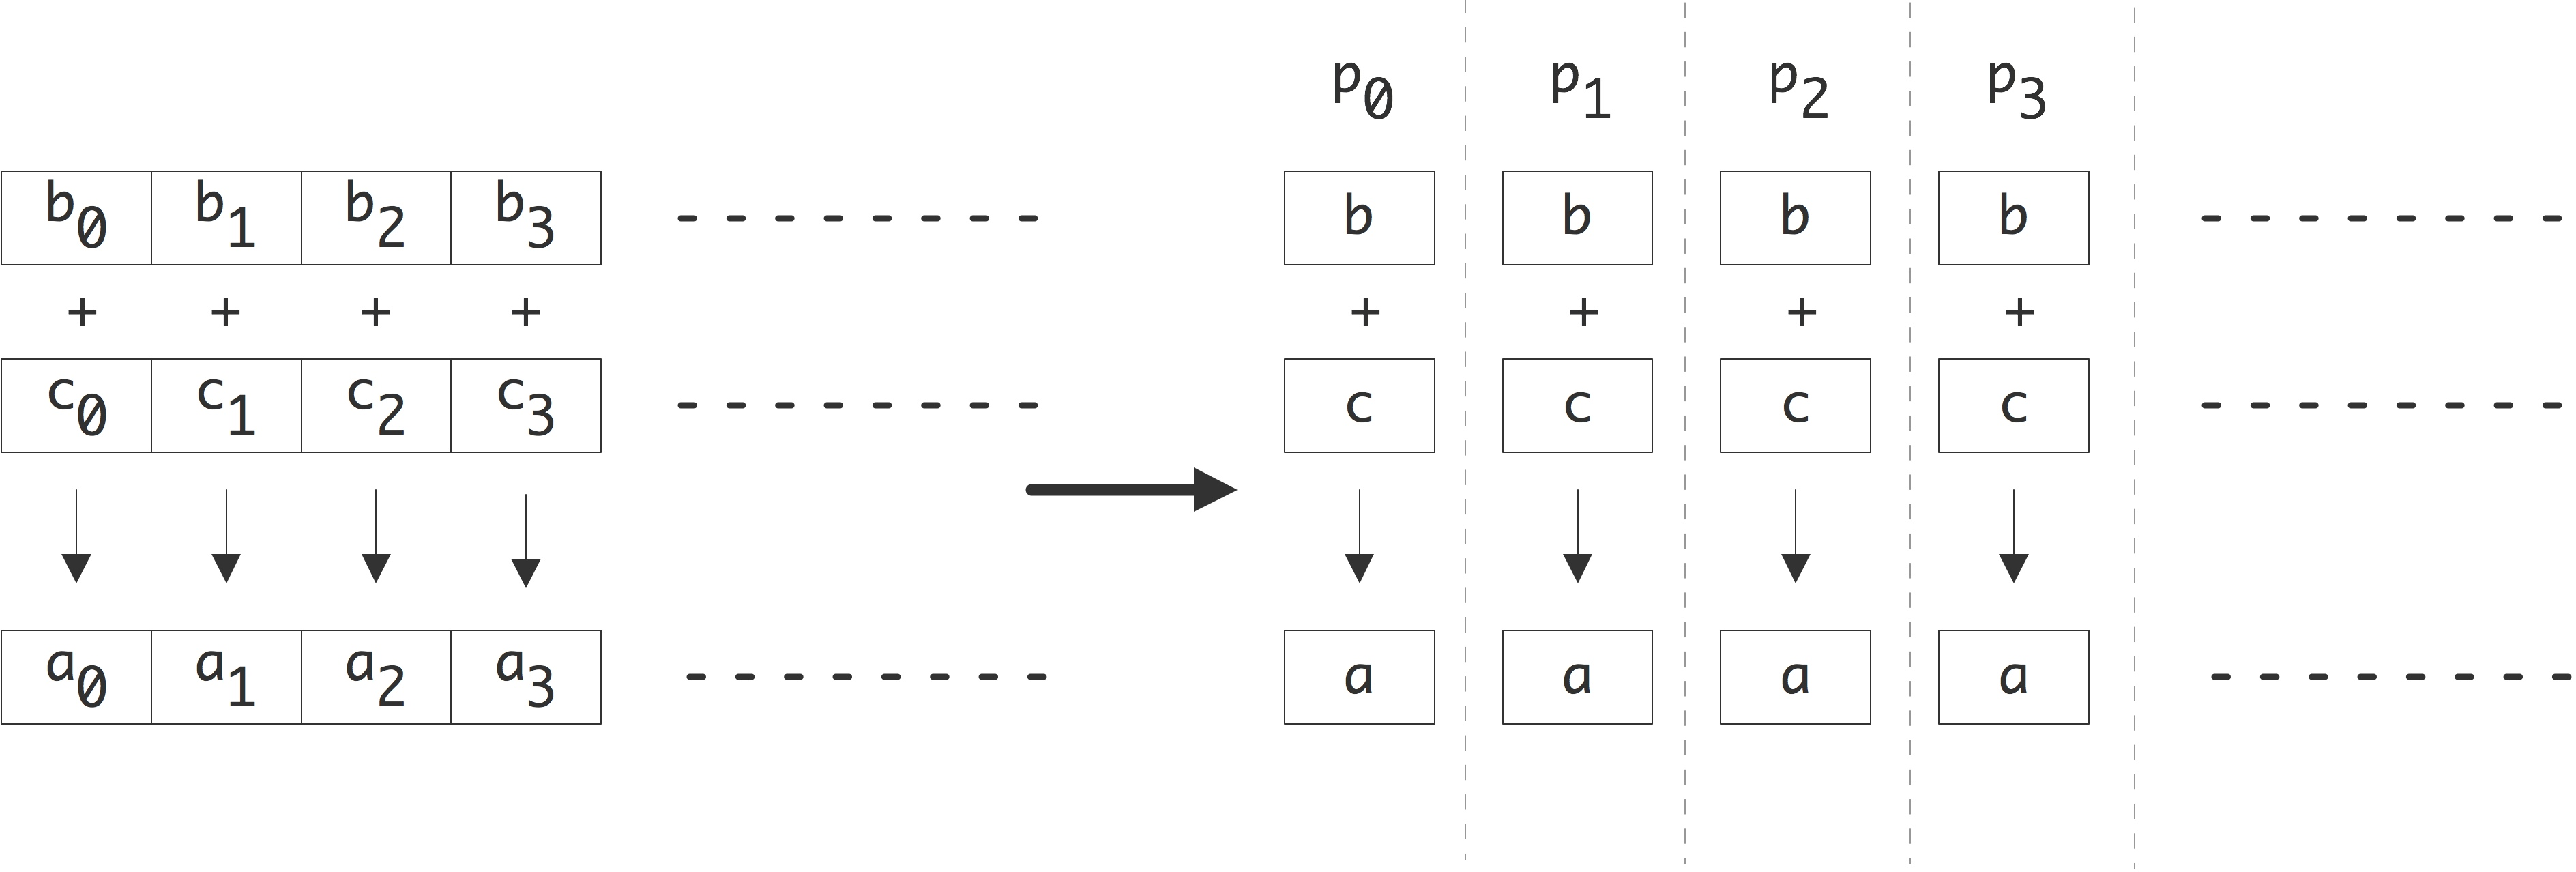
\includegraphics[scale=.07]{parallel-add}

Parallel: every processing element does
\begin{lstlisting}
for ( i in my_subset_of_indices )
  a[i] = b[i] + c[i];
\end{lstlisting}
  Time goes down linearly with processors
\end{numberedframe}

\begin{numberedframe}{Differences between operations}
\begin{multicols}{2}
\begin{lstlisting}
for (i=0; i<n; i++)
  a[i] = b[i] + c[i];
\end{lstlisting}
\columnbreak
\begin{lstlisting}
s = 0;
for (i=0; i<n; i++)
  s += x[i]
\end{lstlisting}
\end{multicols}
  \begin{itemize}
  \item Compare operation counts
  \item Compare behavior on single processor. What about multi-core?
  \item Other thoughts about parallel execution?
  \end{itemize}
\end{numberedframe}

\begin{numberedframe}{Summing}
\begin{multicols}{2}
    Naive algorithm
\begin{lstlisting}
s = 0;
for (i=0; i<n; i++)
  s += x[i]
\end{lstlisting}
\columnbreak
Recoding
\begin{lstlisting}
for (s=2; s<n; s*=2)
  for (i=0; i<n; i+=s)
    x[i] += x[i+s/2]
\end{lstlisting}
\end{multicols}
  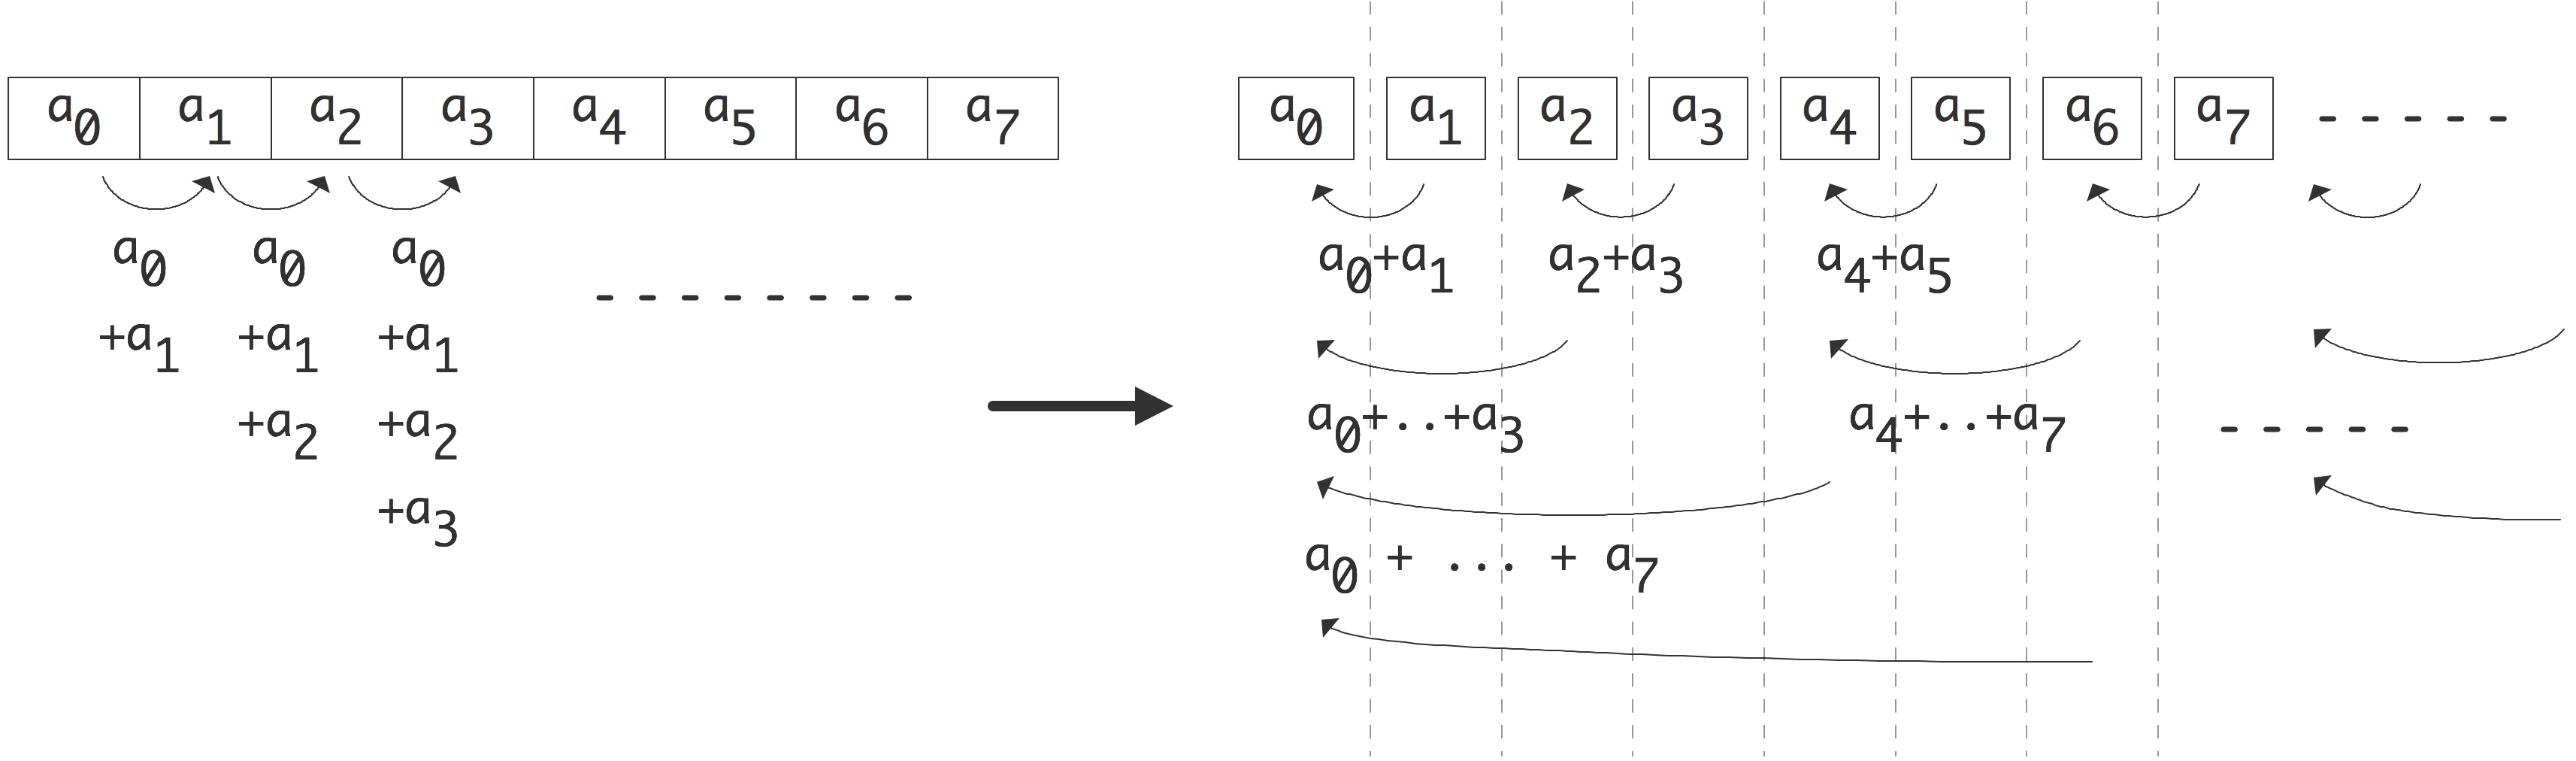
\includegraphics[scale=.1]{parallel-sum}
\end{numberedframe}

\begin{numberedframe}{And then there is hardware}
  Topology of the processors:

  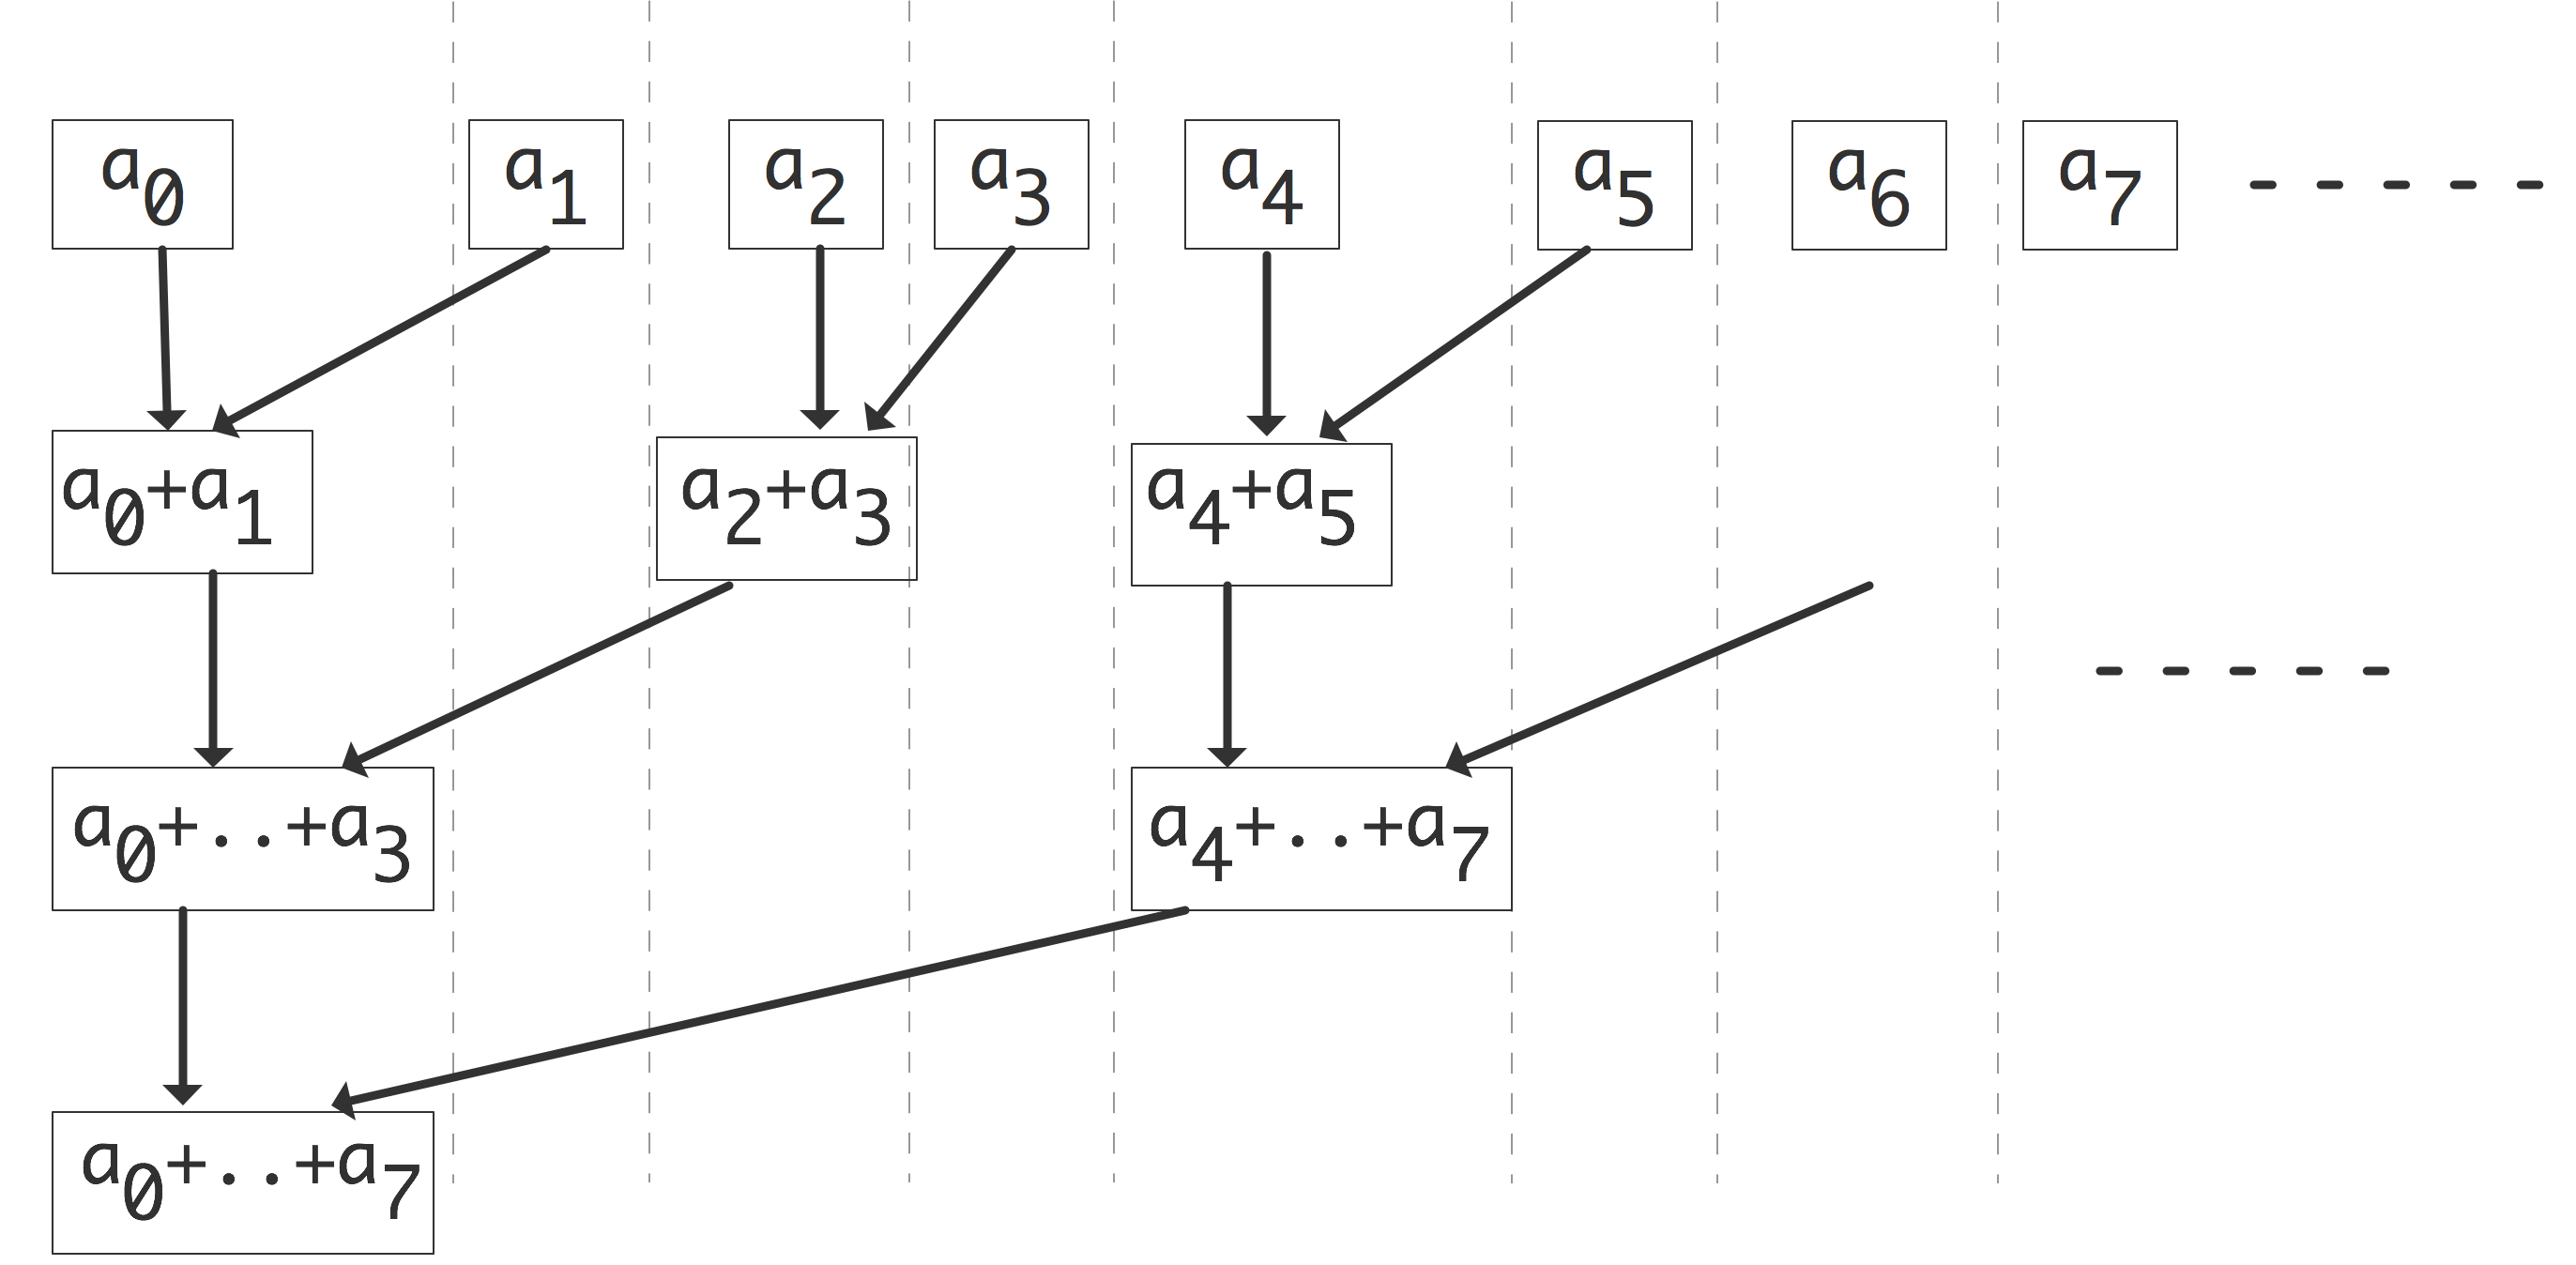
\includegraphics[scale=.1]{parallel-sum-graph}

  increasing distance: limit on parallel speedup
\end{numberedframe}

\Level 1 {Theoretical concepts}

\Level 2 {Efficiency and scaling}

\begin{numberedframe}{Speedup}
  \begin{itemize}
  \item Single processor time $T_1$, on $p$ processors $T_p$
  \item speedup is $S_p=T_1/T_p$, $S_P\leq p$
  \item efficiency is $E_p=S_p/p$, $0< E_p\leq 1$
  \end{itemize}
  But:
\begin{itemize}
\item Is $T_1$ based on the same algorithm? The parallel code?
\item Sometimes superlinear speedup.
\item Is $T_1$ measurable? Can the problem be run on a single processor?
\end{itemize}
\end{numberedframe}

\begin{numberedframe}{Amdahl's law}
  Let's assume that part of the application can be parallelized, part not. (Examples?)
  \begin{itemize}
  \item $F_s$ sequential fraction, $F_p$ parallelizable fraction
  \item $F_s+F_p=1$
  \end{itemize}
  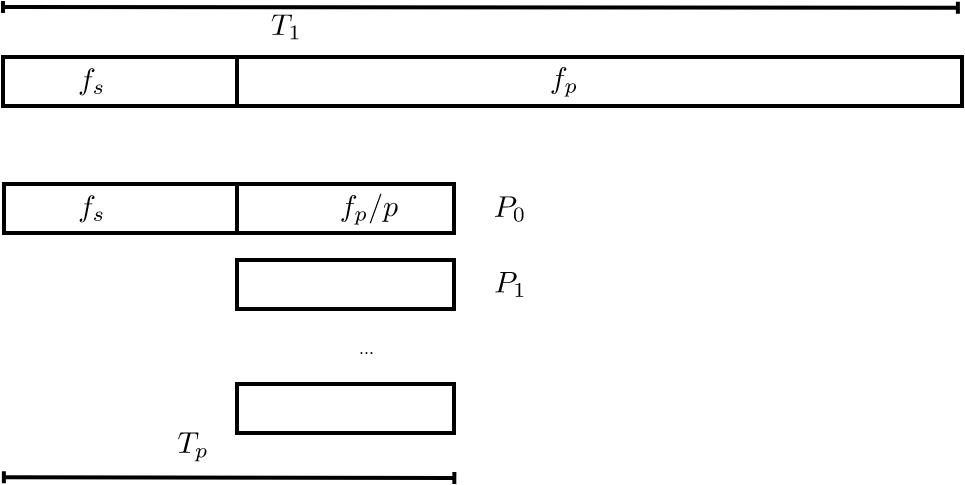
\includegraphics[scale=.3]{amdahl}
\end{numberedframe}

\begin{numberedframe}{Amdahl's law, analysis}
  \begin{itemize}
  \item $F_s$ sequential fraction, $F_p$ parallelizable fraction
  \item $F_s+F_p=1$
  \item $T_1 = (F_s+F_p)T_1 = F_sT_1 + F_pT_1 $
  \item Amdahl's law: $T_p = F_sT_1 + F_pT_1/p $
  \item $P\rightarrow\infty$: $T_P\downarrow T_1F_s$
  \item Speedup is limited by $S_P\leq 1/F_s$,
    efficiency is a decreasing function $E\sim 1/P$.
  %\item loglog plot: straigth line with slope~$-1$
  \end{itemize}  
  Do you see problems with this?
\end{numberedframe}

\begin{numberedframe}{Amdahl's law with communication overhead}
  \begin{itemize}
  \item Communication independent of $p$: $T_p= T_1(F_s+F_p/P) +T_c$
  \item assume fully parallelizable: $F_p=1$
  \item then  $S_p=\frac{T_1}{T_1/p+T_c}$
  \item For reasonable speedup: $T_c\ll T_1/p$ or $p\ll
    T_1/T_c$:\\ number of processors limited by ratio of scalar
    execution time and communication overhead
  \end{itemize}
\end{numberedframe}

\begin{numberedframe}{Gustafson's law}
  Reconstruct the sequential execution from the parallel, then analyze efficiency.

  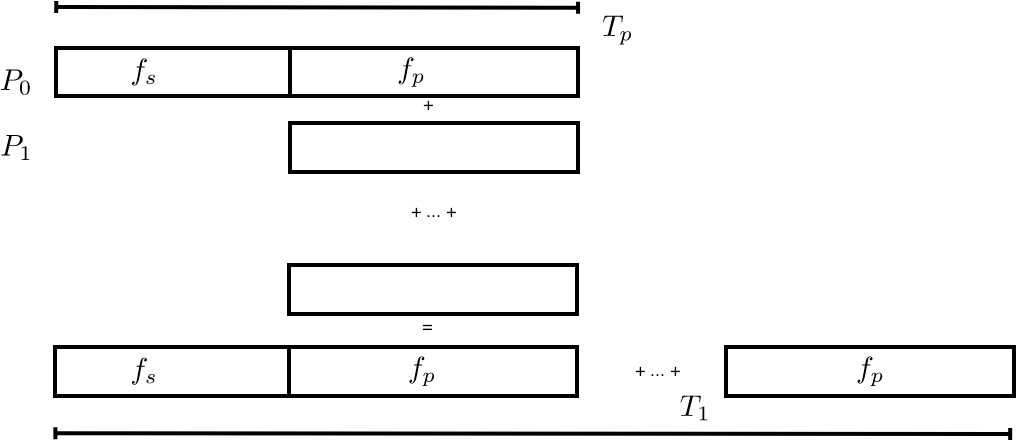
\includegraphics[scale=.3]{gustafson}
\end{numberedframe}

\begin{numberedframe}{Gustafson's law}
  \begin{itemize}
  \item Let $T_p=F_s+F_p\equiv 1$
  \item then $T_1=F_s+p\cdot F_p$
  \item Speedup: \[ S_p=\frac{T_1}{T_p}=\frac{F_s+p\cdot F_p}{F_s+F_p}
    = F_s+p\cdot F_p = p-(p-1)\cdot F_s. 
    \]
    slowly decreasing function of $p$
  \end{itemize}
\end{numberedframe}

\begin{numberedframe}{Scaling}
  \begin{itemize}
  \item Amdahl's law: strong scaling\\
    same problem over increasing processors
  \item Often more realistic: weak scaling\\
    increase problem size with number of processors,\\
    for instance keeping memory constant
  \item Weak scaling: $E_p>c$
  \item example (below): dense linear algebra
  \end{itemize}
\end{numberedframe}

\begin{numberedframe}{Simulation scaling}

  \begin{itemize}
  \item Assumption: simulated time~$S$, running time~$T$ constant, now increase precision
  \item  $m$ memory per processor, and $P$ the number of processors
    \[ M=Pm\qquad\hbox{total memory.} \]
    $d$ the number of space dimensions of the problem, typically 2~or~3,
    \[ \Delta x = 1/M^{1/d}\qquad\hbox{grid spacing.} \]
  \item stability:
    \[ \Delta t=
    \begin{cases}
      \Delta x=1\bigm/M^{1/d}&\hbox{hyperbolic case}\\
      \Delta x^2=1\bigm/M^{2/d}&\hbox{parabolic case}
    \end{cases}
    \]
    With a simulated time $S$:
    \[ k=S/\Delta t\qquad \hbox{time steps.} \]
  \end{itemize}     
\end{numberedframe}

\begin{numberedframe}{Simulation scaling con'td}
  \begin{itemize}
  \item Assume time steps parallelizable
    \[ T=kM/P=\frac{S}{\Delta t}m. \]
    Setting $T/S=C$, we find
    \[ m=C\Delta t, \]
    memory per processor goes down.
    \[ m=C\Delta t = c
    \begin{cases}
      1\bigm/M^{1/d}&\hbox{hyperbolic case}\\
      1\bigm/M^{2/d}&\hbox{parabolic case}
    \end{cases}
    \]
  \item Substituting $M=Pm$, we find ultimately
    \[ m = C
    \begin{cases}
      1\bigm/P^{1/(d+1)}&\hbox{hyperbolic}\\
      1\bigm/P^{2/(d+2)}&\hbox{parabolic}
    \end{cases}
    \]
  \end{itemize}
\end{numberedframe}

\begin{exercise}{Linpack scaling}
  \label{ex:scal-linpack}
  Explore simulation scaling in the context of the
  \indextermbus{Linpack}{benchmark},
  that is, Gaussian elimination.
  Ignore the system solving part and
  only consider the factorization part.
  \begin{enumerate}
  \item Suppose you have a single core machine, 
    and your benchmark run takes time~$T$ with $M$~words of memory
    Now you buy a processor that is twice as fast, and you want to do a
    benchmark run that again takes time~$T$. How much memory do you need?
  \item Now suppose you have a machine with $P$ processors,
    each with $M$ memory, and your benchmark run takes time~$T$.
    You buy a machine with $2P$ processors, of the same clock speed
    and core count, and you want to do a benchmark run, again
    taking time~$T$. How much memory does each node take?
  \end{enumerate}
\end{exercise}
%{ex:scal-linpack}

\begin{numberedframe}{Critical path}
  \begin{itemize}
  \item The sequential fraction contains a \textsl{critical path}:
    a~sequence of operations that depend on each other.
  \item Example?
  \item $T_\infty=$ time with unlimited processors: length of critical path.
  \end{itemize}
  \hbox to \textwidth{
    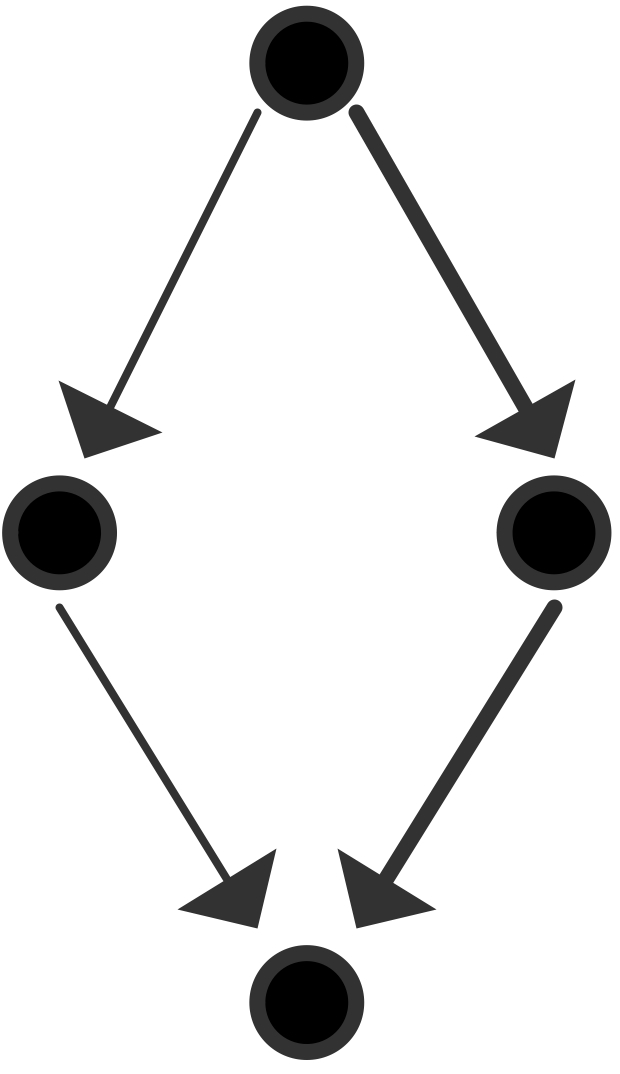
\includegraphics[scale=.05]{critical1} \hss
    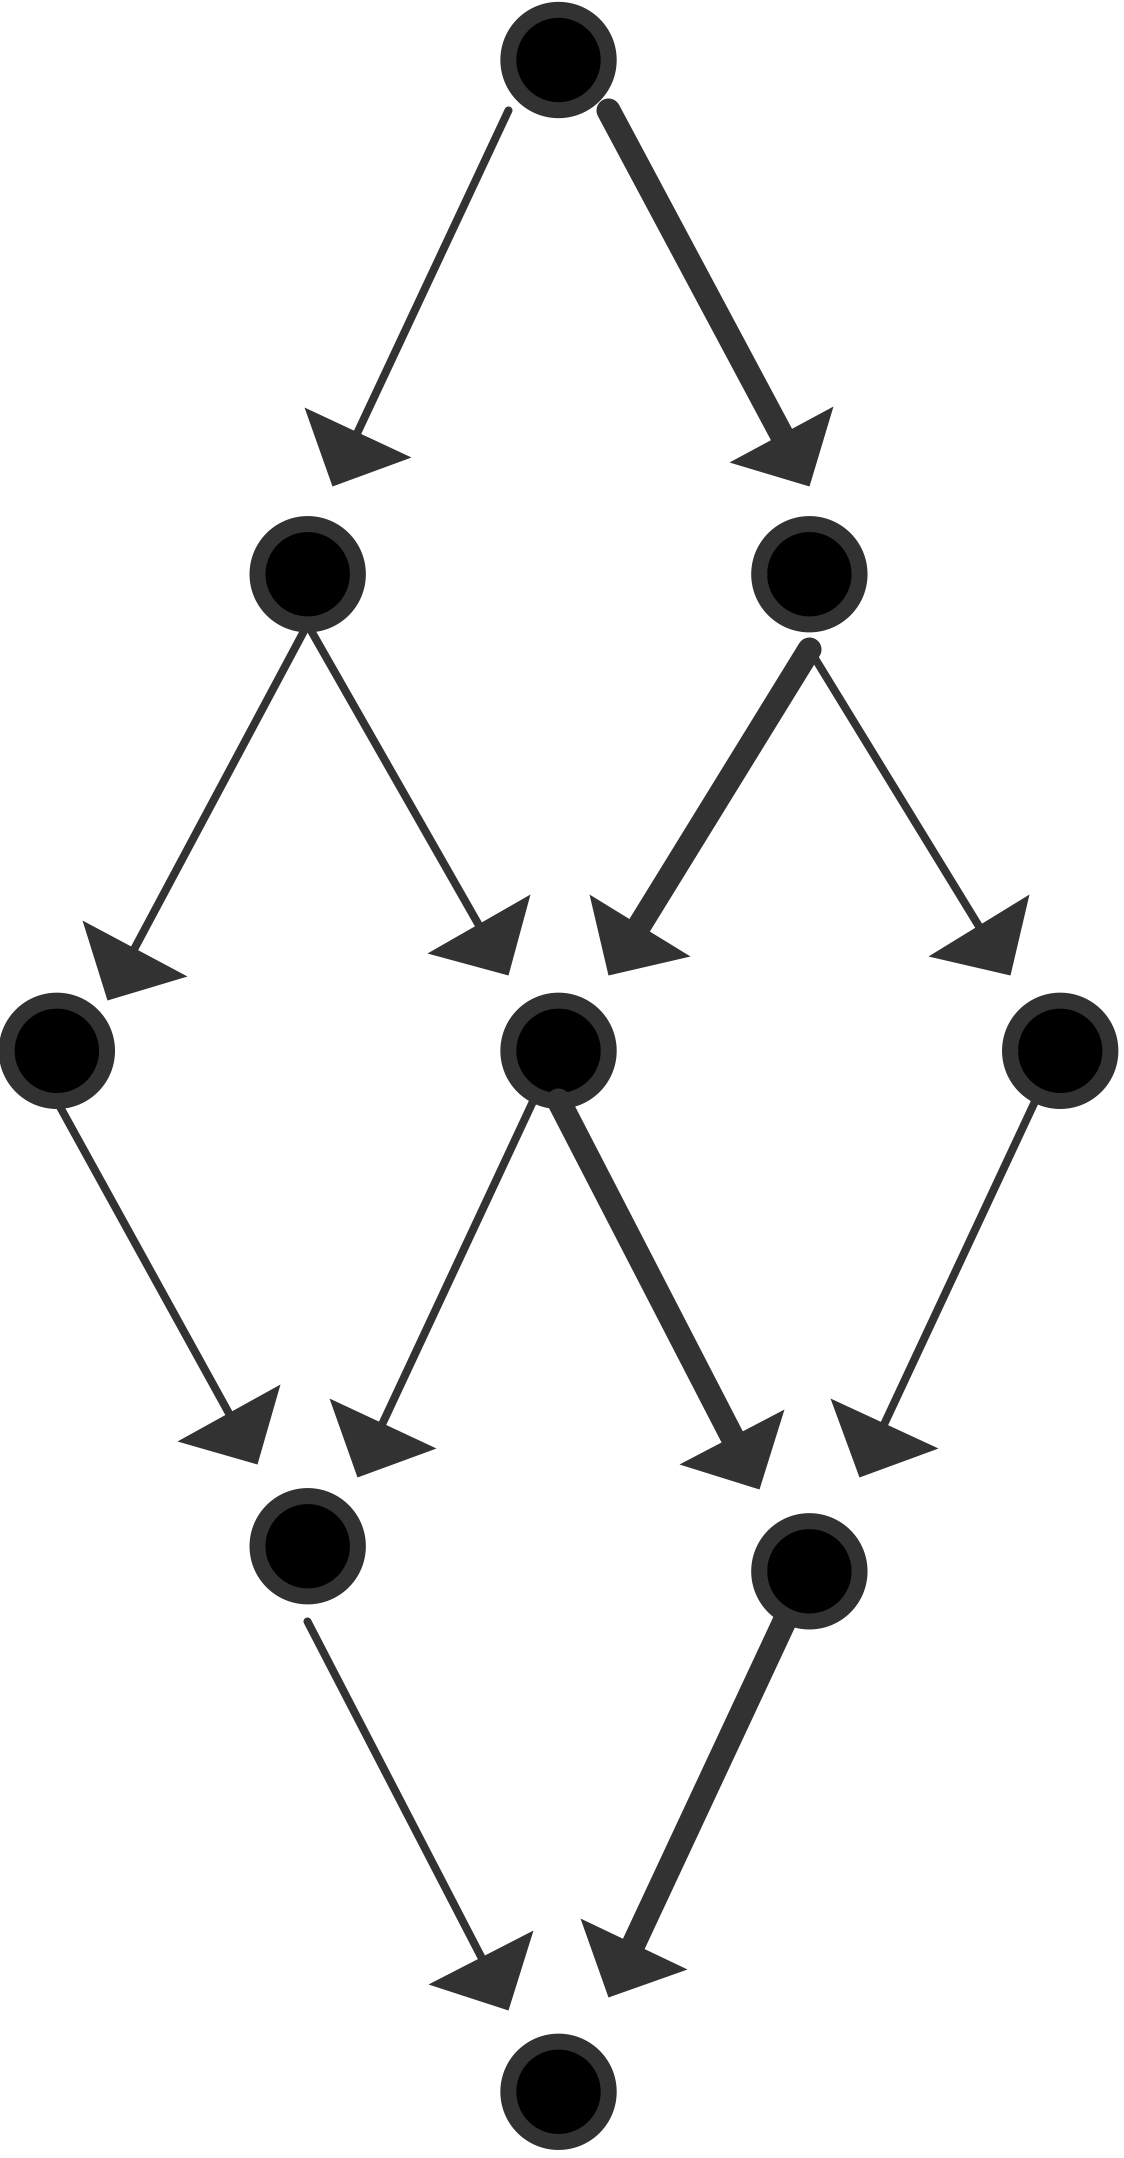
\includegraphics[scale=.04]{critical2}
  }
\end{numberedframe}

\begin{numberedframe}{Brent's theorem}
    Let $m$ be the total number of tasks, $p$~the number of processors,
  and $t$ the length of a \indexterm{critical path}. Then
  the computation can be done in \[ T_p \leq t +\frac{m-t}{p}. \]

  \begin{itemize}
  \item Time equals the length of the critical path~\ldots
  \item \ldots~plus the remaining work as parallel as possible.
  \end{itemize}
\end{numberedframe}

\begin{exercise}{Linpack analysis}
  Apply Brent's theorem to Gaussian elimination,
  assuming that add/multiply/division all take one unit time.

  What is the critical path; what is its length; what is the resulting upper bound
  on the parallel runtime?
  
  How many processors could you theoretically use?
  What speedup and efficiency does that give?
\end{exercise}

\Level 2 {Granularity}

\begin{numberedframe}{Definition}
  Definition: granularity is the measure for how many 
  operations can be performed between synchronizations
\end{numberedframe}

\begin{numberedframe}{Instruction level parallelism}
\[ 
\begin{array}{l}
  a\leftarrow b+c\\ d\leftarrow e*f
\end{array}
\]
For the compiler / processor to worry about
\end{numberedframe}

\begin{numberedframe}{Data parallelism}
\begin{lstlisting}
for (i=0; i<1000000; i++)
  a[i] = 2*b[i];
\end{lstlisting}
\begin{itemize}
\item Array processors, vector instructions, pipelining, GPUs
\item Sometimes harder to discover
\item Often used mixed with other forms of parallelism
\end{itemize}
\end{numberedframe}

\begin{numberedframe}{Task-level parallelism}
  \begin{displayprocedure}{SearchInTree}{root}
  \SetKw{optimal}{optimal}\SetKw{exit}{exit}\SetKw{search}{SearchInTree}\SetKw{parl}{parallel}
  \eIf{\optimal(root)}{\exit}
  {\parl: \search(leftchild),\search(rightchild)}
\end{displayprocedure}

Unsynchronized tasks: fork-join\\
general scheduler

\begin{displayalgorithm}
  \While{there are tasks left}{
    wait until a processor becomes inactive;\\
    spawn a new task on it}
\end{displayalgorithm}
\end{numberedframe}

\begin{numberedframe}{Conveniently parallel}
  Example: Mandelbrot set

  Parameter sweep,\\
  often best handled by external tools
\end{numberedframe}

\begin{numberedframe}{Medium-grain parallelism}
Mix of data parallel and task parallel
\begin{lstlisting}
my_lower_bound = // some processor-dependent number
my_upper_bound = // some processor-dependent number
for (i=my_lower_bound; i<my_upper_bound; i++)
  // the loop body goes here
\end{lstlisting}
\end{numberedframe}

\Level 1 {The SIMD/MIMD/SPMD/SIMT model for parallelism}

\begin{numberedframe}{Flynn Taxonomy}
  Consider instruction stream and data stream:
  \begin{itemize}
  \item SISD: single instruction single data\\
    used to be single processor, now single core
  \item MISD: multiple instruction single data\\
    redundant computing for fault tolerance?
  \item SIMD: single instruction multiple data\\
    data parallelism, pipelining, array processing, vector instructions
  \item MIMD: multiple instruction multiple data\\
    independent processors, clusters, MPPs
  \end{itemize}
\end{numberedframe}

\begin{numberedframe}{SIMD}
  \begin{itemize}
  \item Relies on streams of identical operations
  \item See pipelining
  \item Recurrences hard to accomodate
  \end{itemize}
\end{numberedframe}

\begin{numberedframe}{SIMD: array processors}
  \begin{columns}
    \begin{column}{.5\textwidth}
      Technology going back to the 1980s: FPS, MasPar, CM, GoodYear

      Major advantage: simplification of processor
    \end{column}
    \begin{column}{.5\textwidth}
      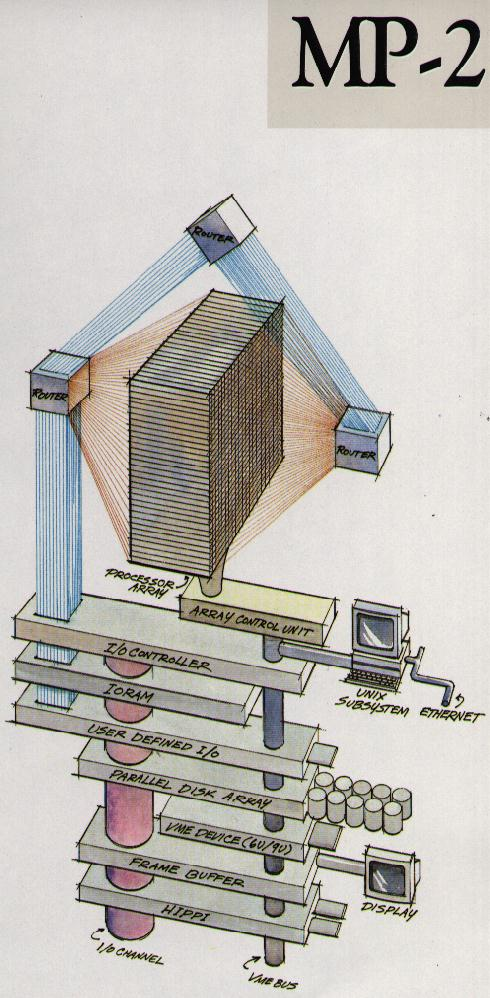
\includegraphics[scale=.2]{maspar2}
    \end{column}
  \end{columns}
\end{numberedframe}

\begin{numberedframe}{SIMD as vector instructions}
  \begin{itemize}
  \item Register width multiple of 8 bytes:
  \item simultaneous processing of more than one operand pair
  \item SSE: 2 operands,
  \item AVX: 4 or 8 operands
  \end{itemize}
  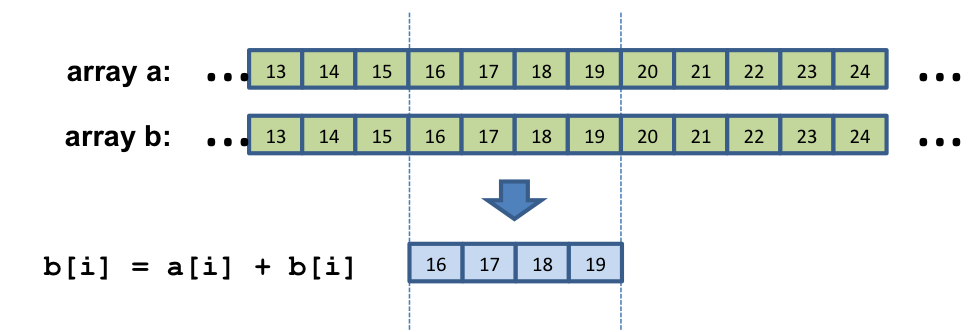
\includegraphics[scale=.7]{avx}
\end{numberedframe}

\begin{numberedframe}{Controlling vector instructions}
\begin{lstlisting}
void func(float *restrict c, float *restrict a,
          float *restrict b, int n)
{
#pragma vector always
  for (int i=0; i<n; i++)
    c[i] = a[i] * b[i];
}
\end{lstlisting}
This needs aligned data (\verb+posix_memalign+)
\end{numberedframe}

\begin{numberedframe}{New branches in the taxonomy}
  \begin{itemize}
  \item SPMD: single program multiple data\\
    the way clusters are actually used
  \item SIMT: single instruction multiple threads\\
    the GPU model
  \end{itemize}
\end{numberedframe}

\begin{numberedframe}{MIMD becomes SPMD}
  \begin{itemize}
  \item MIMD: independent processors, independent instruction streams, independent data
  \item In practice very little true independence: usally the same executable\\
    Single Program Multiple Data
  \item Exceptional example: climate codes
  \item Old-style SPMD: cluster of single-processor nodes
  \item New-style: cluster of multicore nodes, ignore shared caches~/ memory
  \item (We'll get to hybrid computing in a minute)
  \end{itemize}  
\end{numberedframe}

\begin{numberedframe}{GPUs and data paralleism}
  Lockstep in thread block, \\
  single instruction model between streaming processors

  (more about GPU threads later)
\end{numberedframe}

\Level 1 {Characterization of parallelism by memory model}

\begin{numberedframe}{Major types of memory organization, classic}
  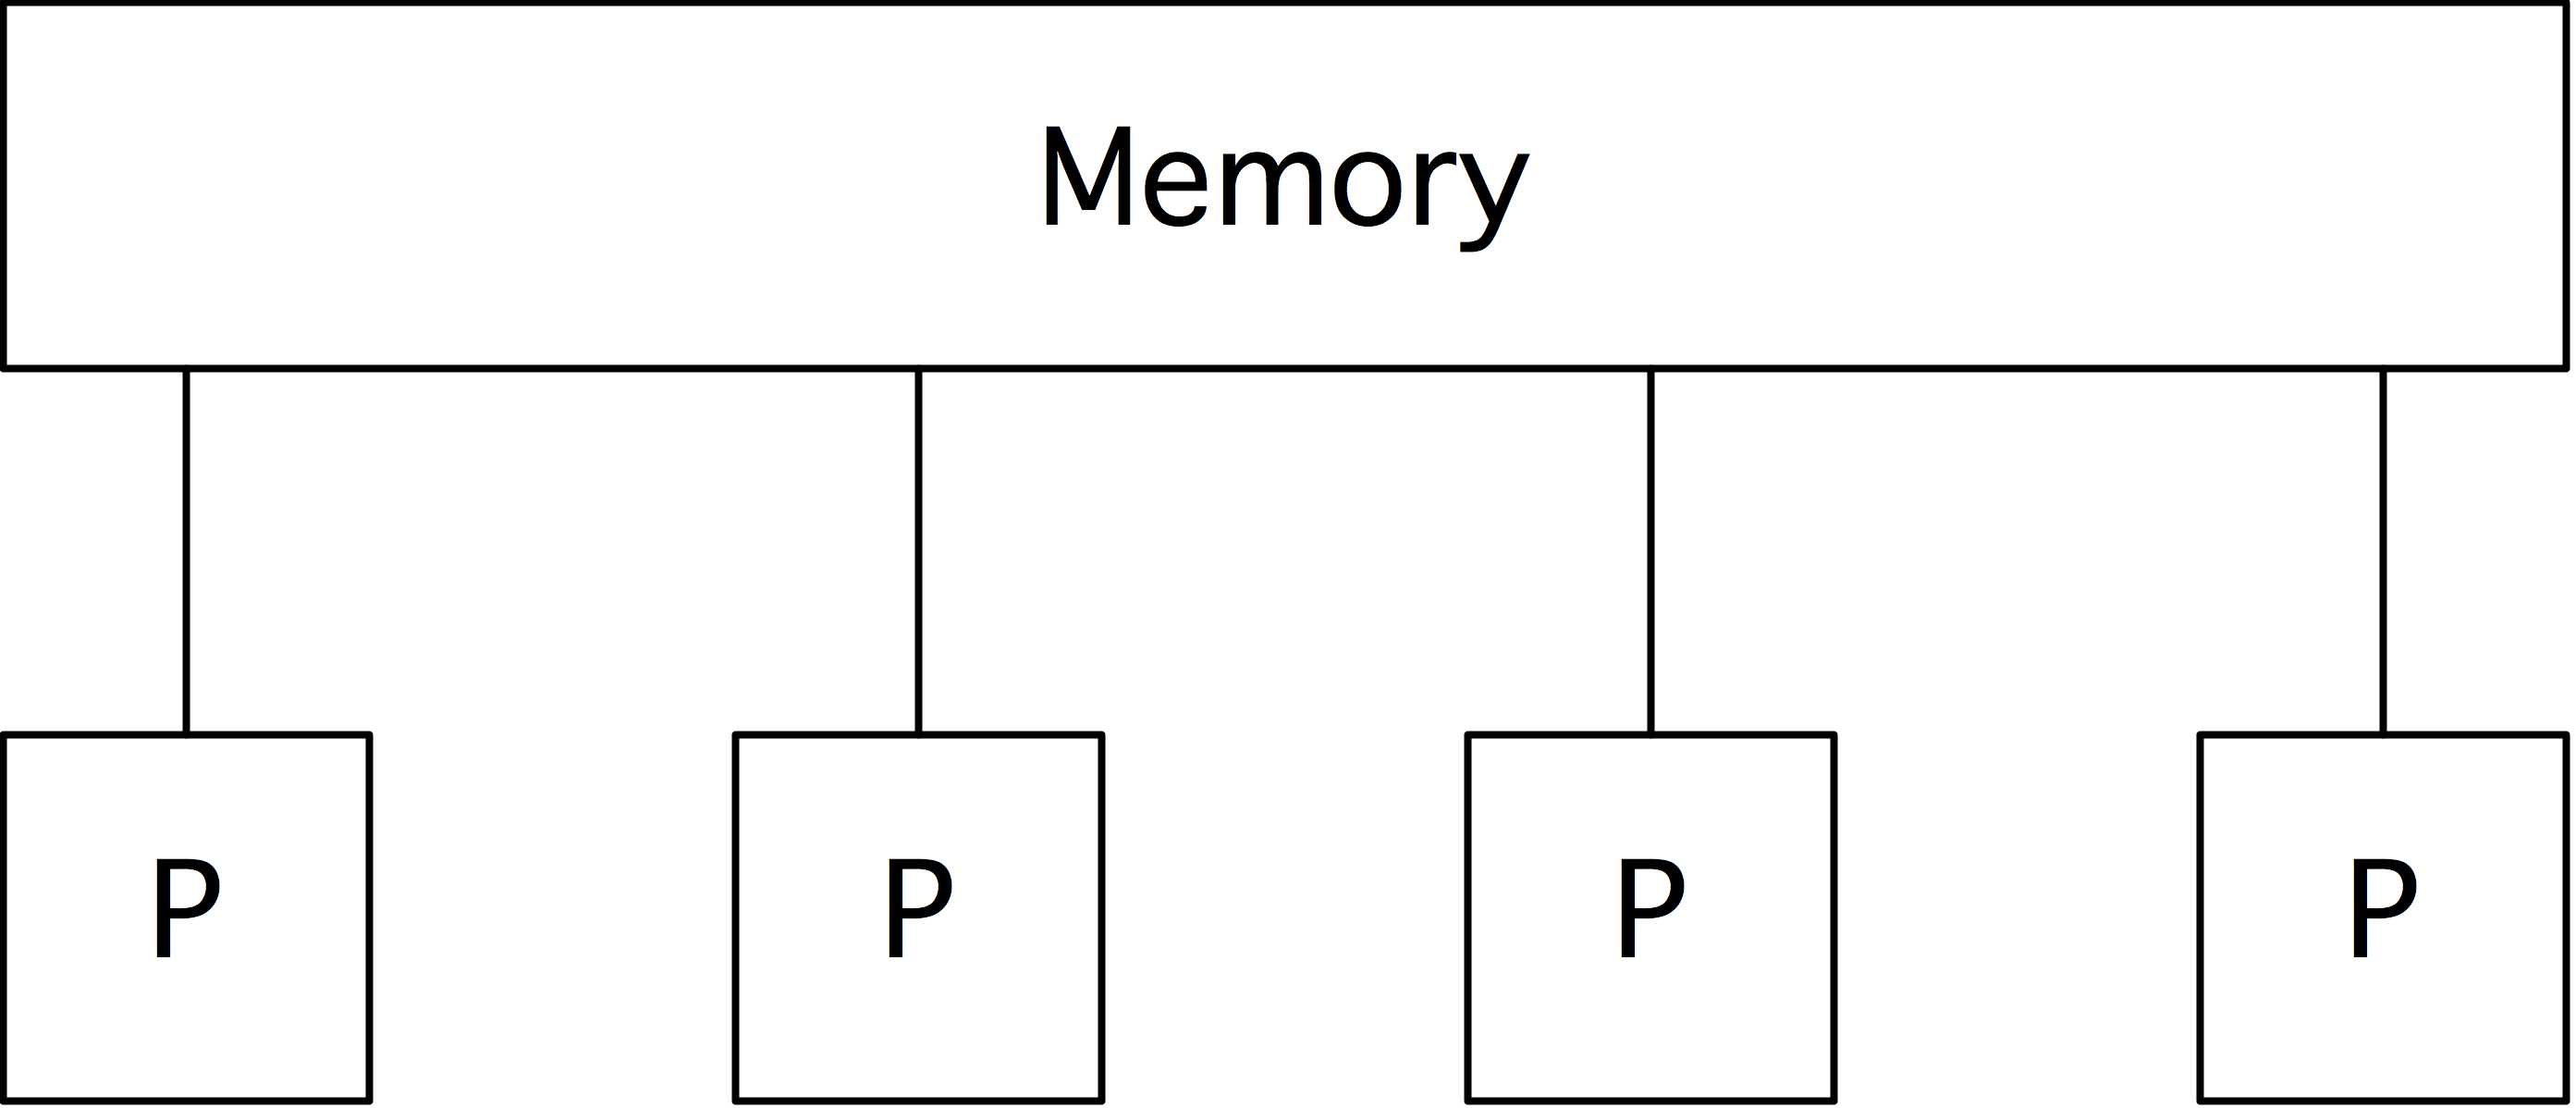
\includegraphics[scale=.05]{arch-shared}

  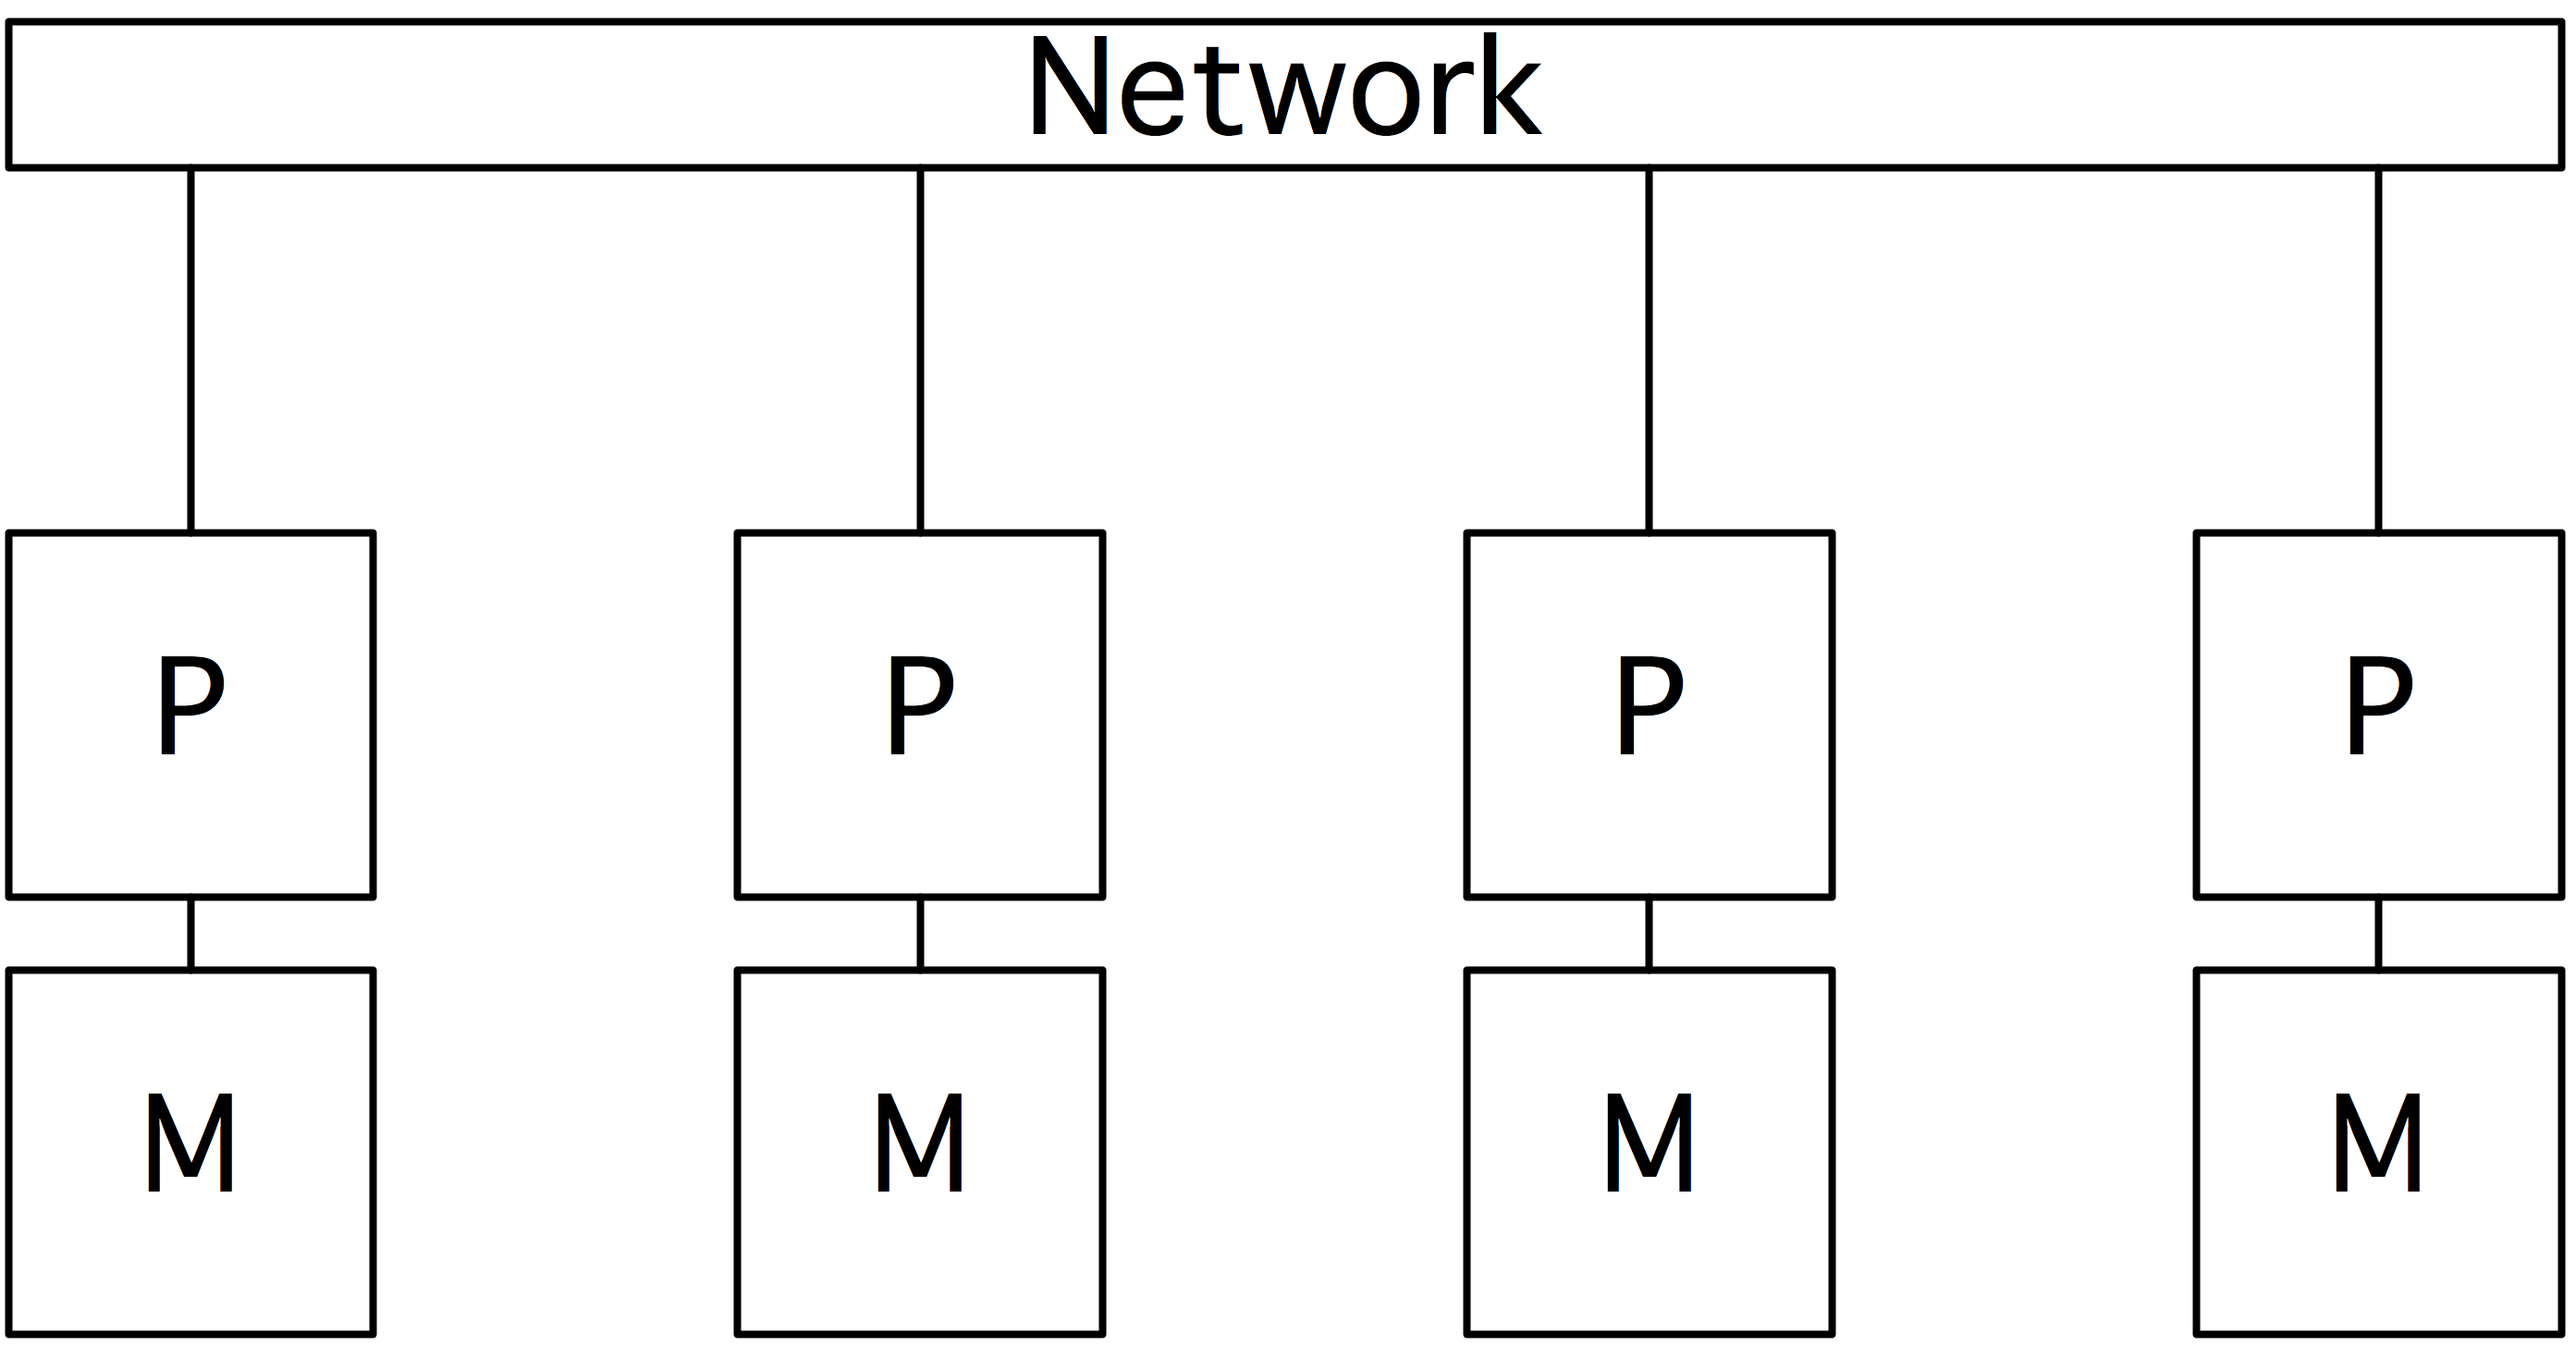
\includegraphics[scale=.05]{arch-distributed}
\end{numberedframe}

\begin{numberedframe}{Major types of memory organization, contemporary}
  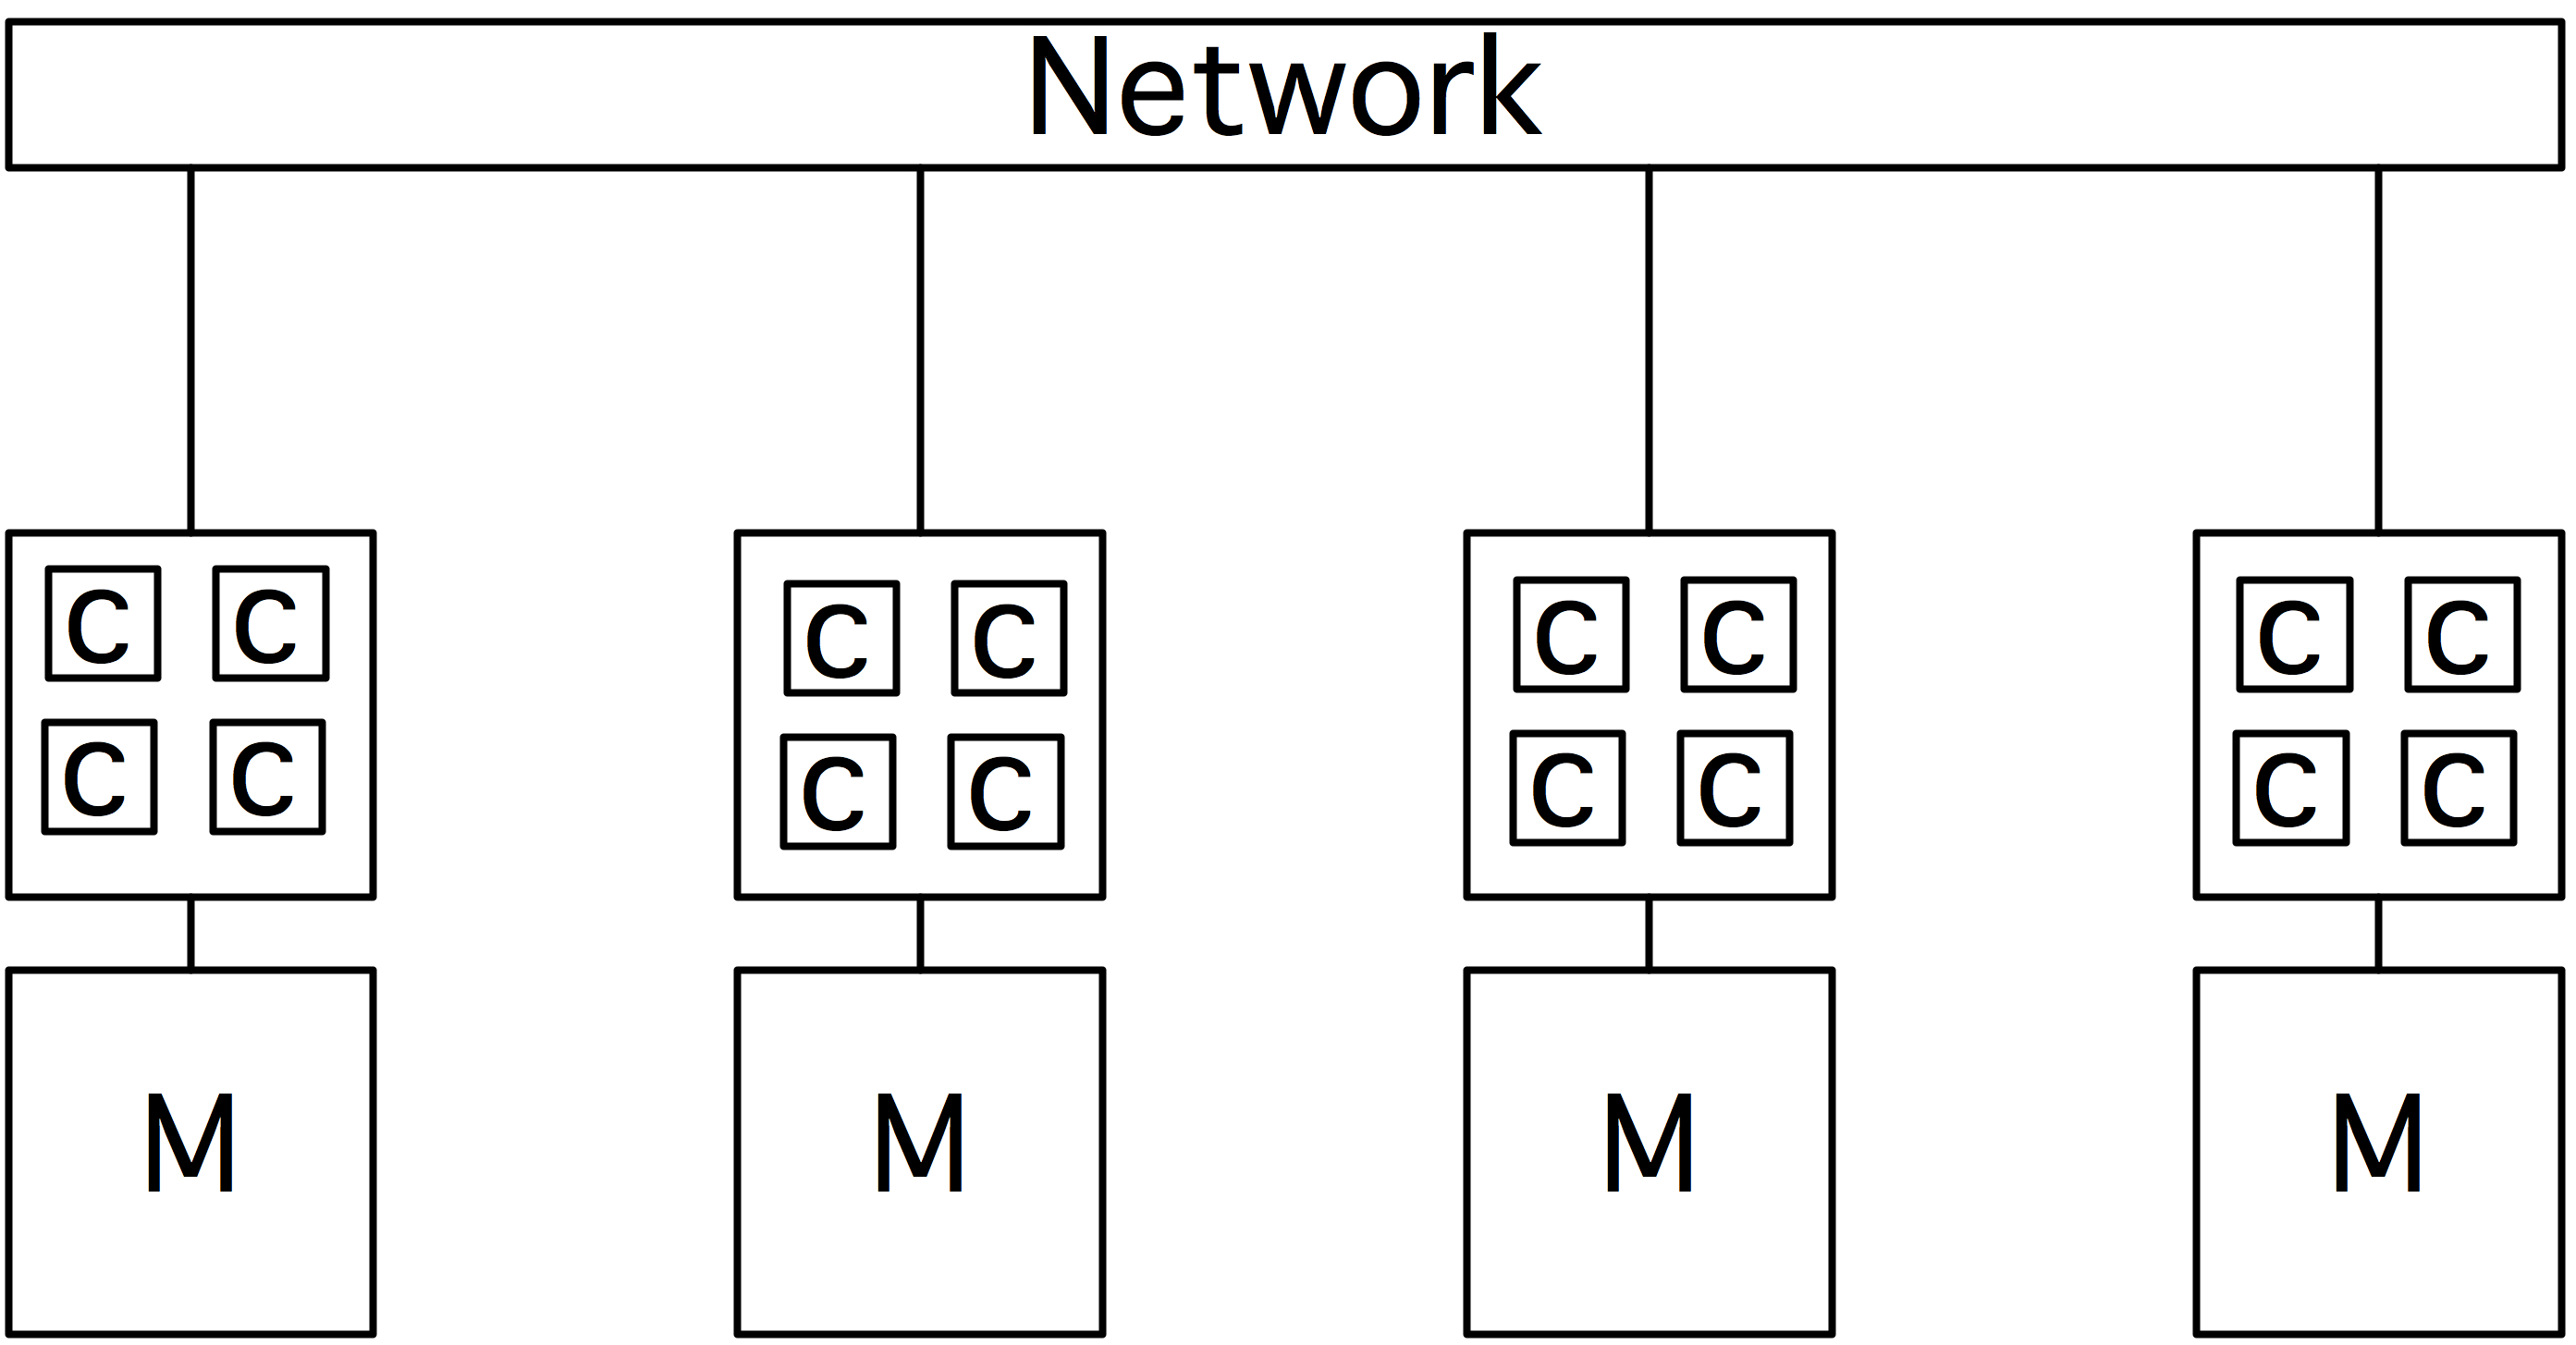
\includegraphics[scale=.05]{arch-multicore}

  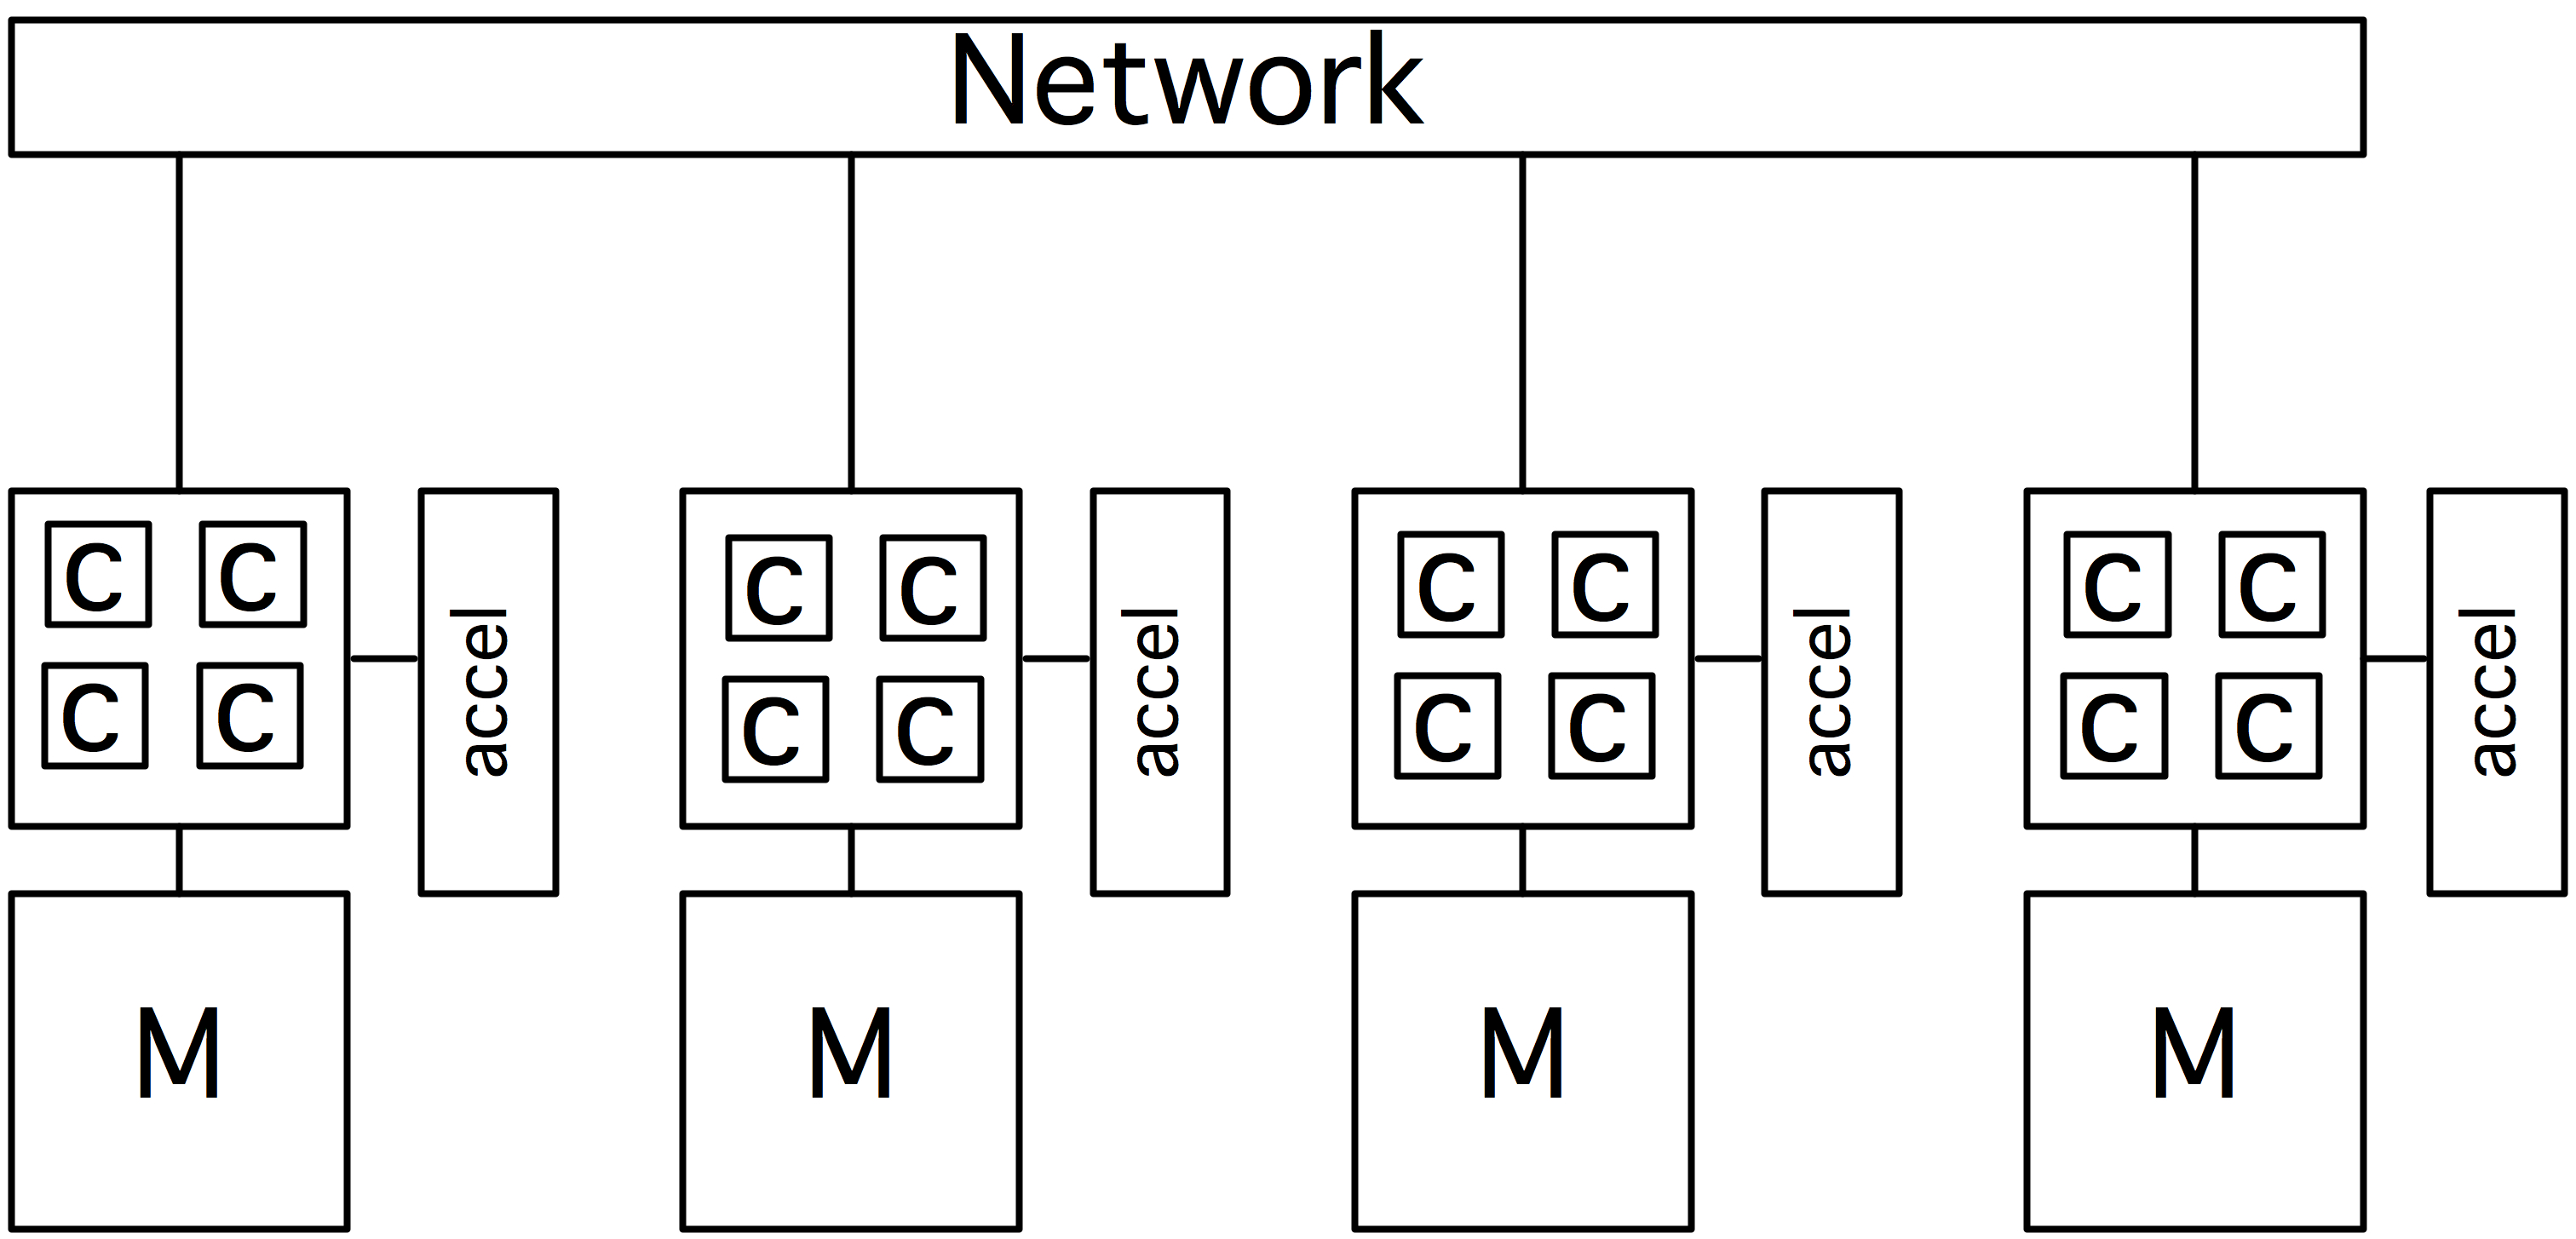
\includegraphics[scale=.05]{arch-accelerator}
\end{numberedframe}

\begin{numberedframe}{Symmetric multi-processing}
  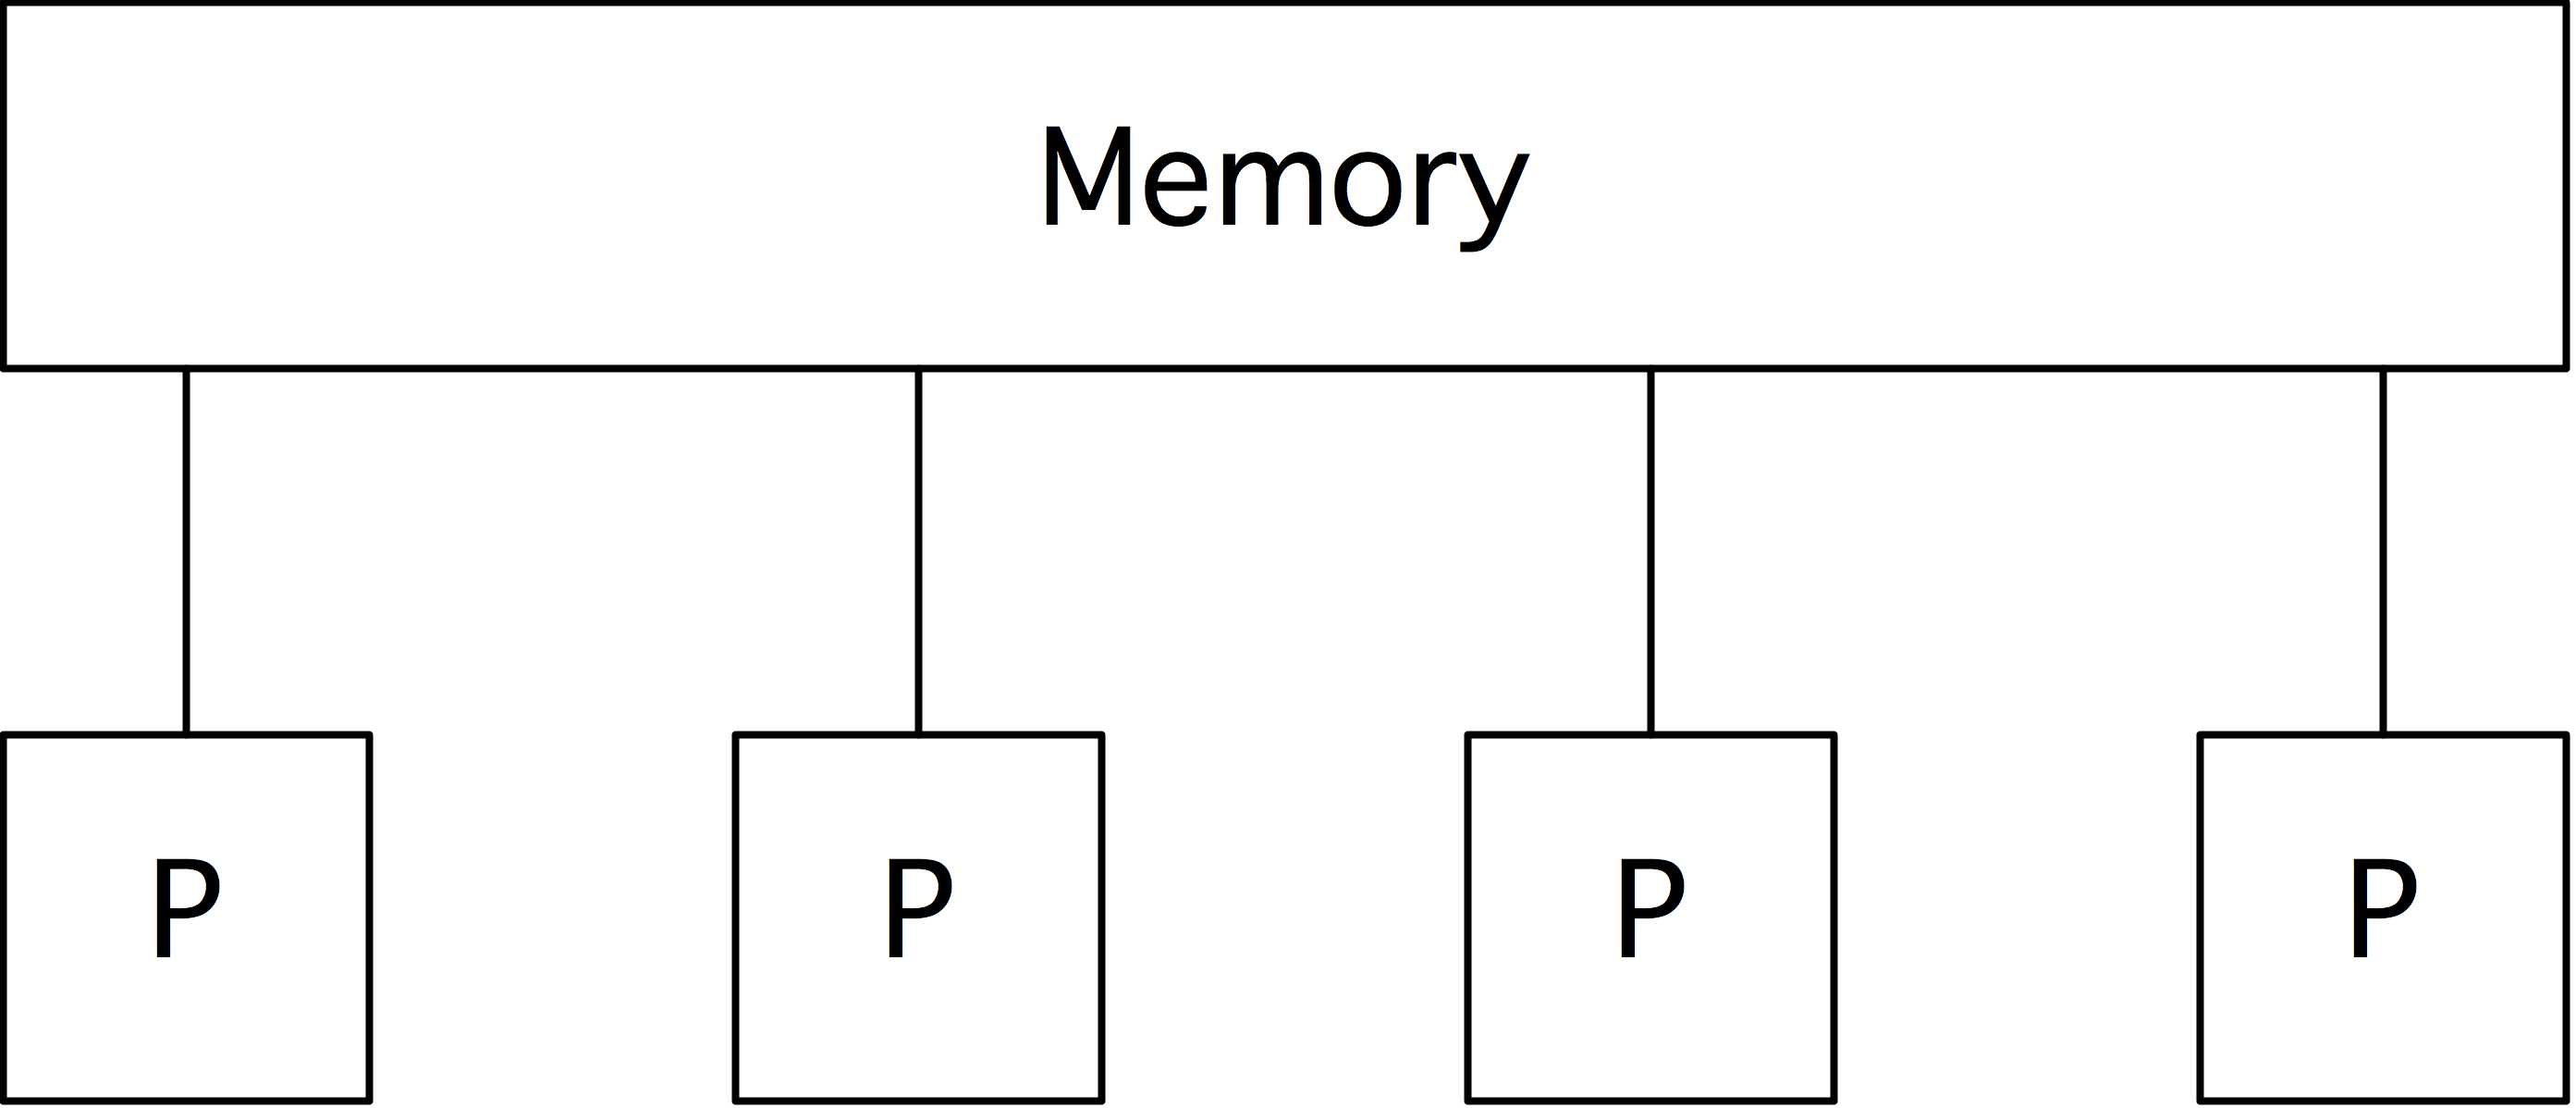
\includegraphics[scale=.05]{arch-shared}
  \begin{itemize}
  \item The ideal case of shared memory:\\
    every address equally accessible
  \item This hasn't existed in a while\\
    (Tim Mattson claims Cray-2)
  \item Danger signs: shared memory programming pretends
    that memory access is symmetric\\
    in fact: hides reality from you
  \end{itemize}
\end{numberedframe}

\begin{numberedframe}{SMP, bus design}
  \begin{itemize}
  \item Bus: all processors on the same wires to memory
  \item Not very scalable: requires slow processors or cache memory
  \item Cache coherence easy by `snooping'
  \end{itemize}
\end{numberedframe}

\begin{numberedframe}{Non-uniform Memory Access}
  Memory is equally programmable, but not equally accessible
  \begin{itemize}
  \item Different caches, different affinity
  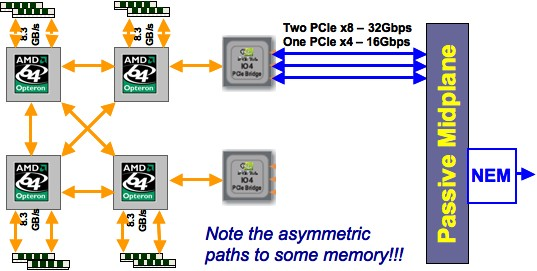
\includegraphics[scale=.4]{ranger-numa}
  \item Distributed shared memory: network latency\\
    ScaleMP and other products {\tiny watch me not believe it}
  \end{itemize}
\end{numberedframe}

\begin{numberedframe}{Picture of NUMA}
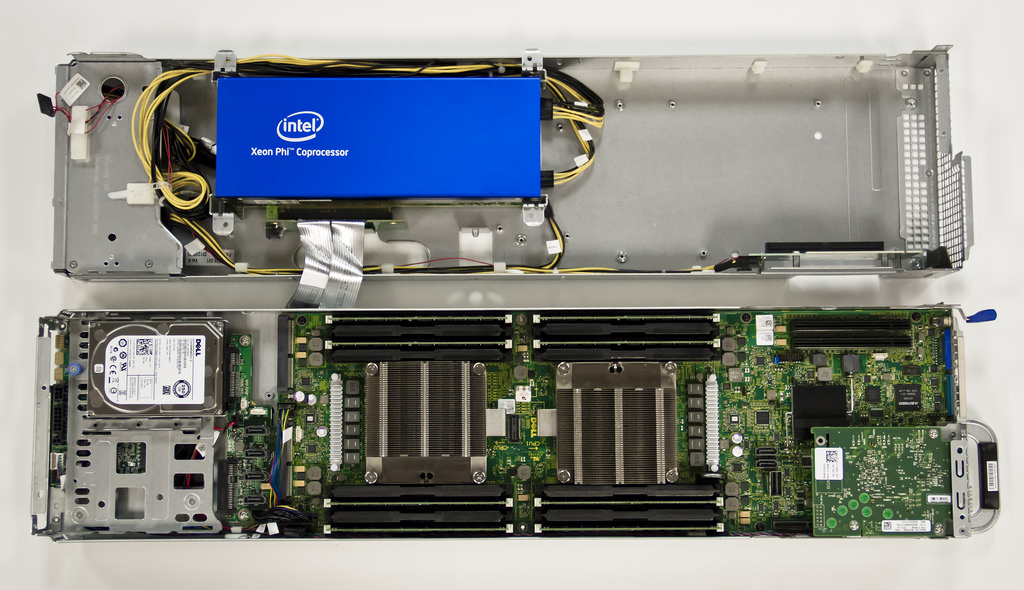
\includegraphics[scale=.3]{zeus_phi}
\end{numberedframe}

\Level 1 {Interconnects and topologies, theoretical concepts}

\begin{numberedframe}{Topology concepts}
  \begin{itemize}
  \item Hardware characteristics
  \item Software requirement
  \item Design: how `close' are processors?
  \end{itemize}
\end{numberedframe}

\begin{numberedframe}{Graph theory}
  \begin{itemize}
  \item Degree: number of connections from one processor to others
  \item Diameter: maximum minimum distance (measured in hops)
  \end{itemize}
\end{numberedframe}

\begin{numberedframe}{Bandwidth}
  \begin{itemize}
  \item Bandwidth per wire is nice, adding over all wires is nice, but\ldots\\
  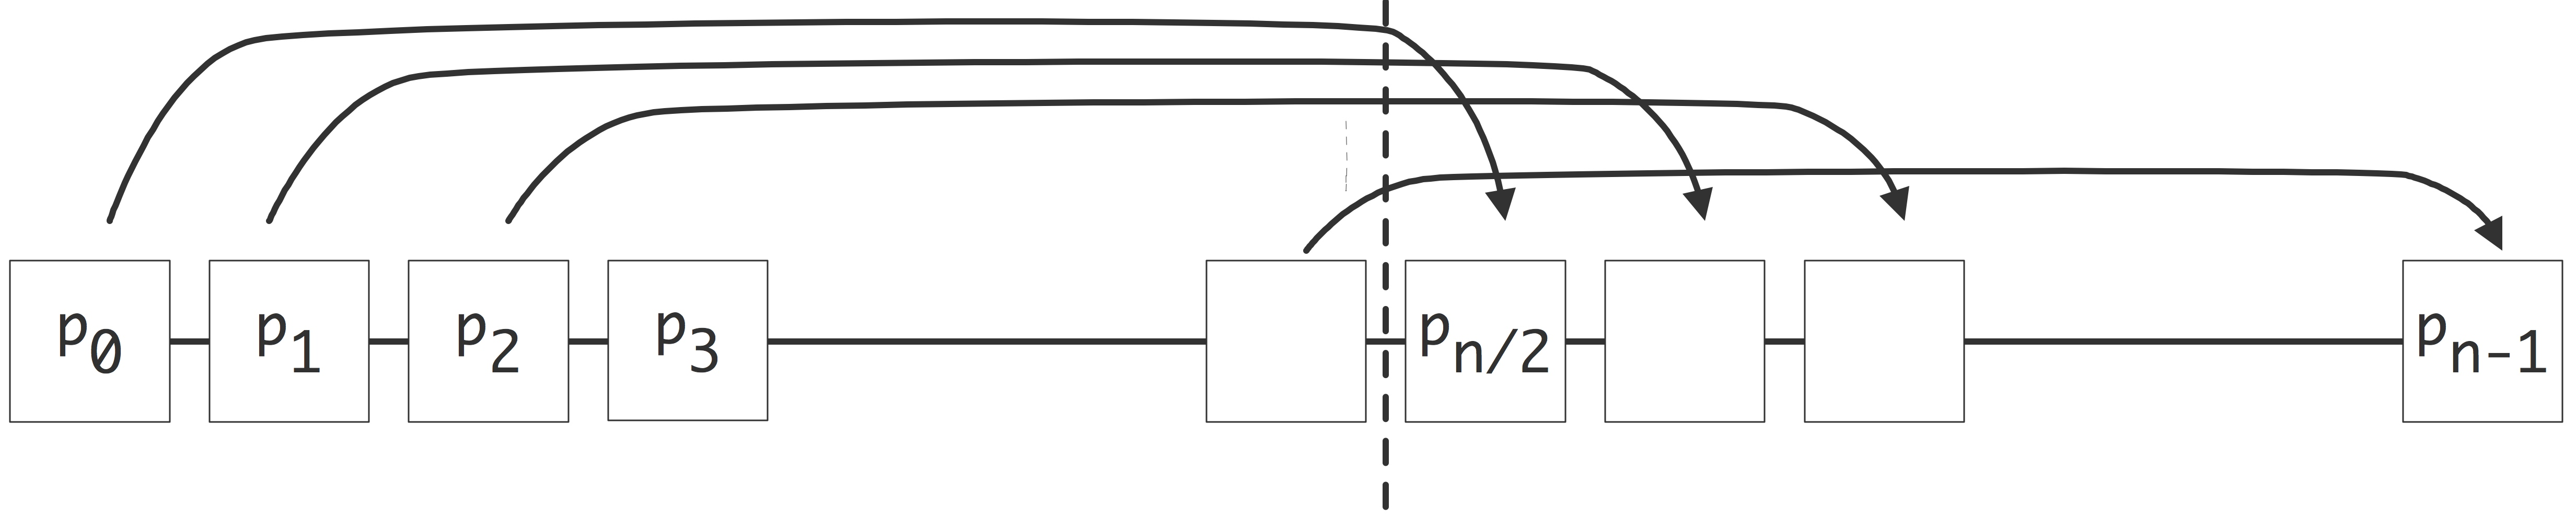
\includegraphics[scale=.05]{contention}
  \item Bisection width: minimum number of wires through a cut
  \item Bisection bandwidth: bandwidth through a bisection
  \end{itemize}
\end{numberedframe}

\begin{numberedframe}{Design 1: bus}
  Already discussed; simple design, does not scale very far
\end{numberedframe}

\begin{numberedframe}{Design 2: linear arrays}
  \begin{itemize}
  \item Degree 2, diameter~$P$, bisection width~$1$
  \item Scales nicely!
  \item but low bisection width
  \end{itemize}
\end{numberedframe}

\begin{exercise}{Broadcast algorithm}
  Flip last bit, flip one before,~\ldots
\end{exercise}

\begin{numberedframe}{Design 3: 2/3-D arrays}
  \begin{itemize}
  \item Degree $2d$, diameter $P^{1/d}$
  \item Natural design: nature is three-dimensional
  \item More dimensions: less contention.\\ K-machine is 6-dimensional
  \end{itemize}
\end{numberedframe}

\begin{numberedframe}{Design 3: Hypercubes}
  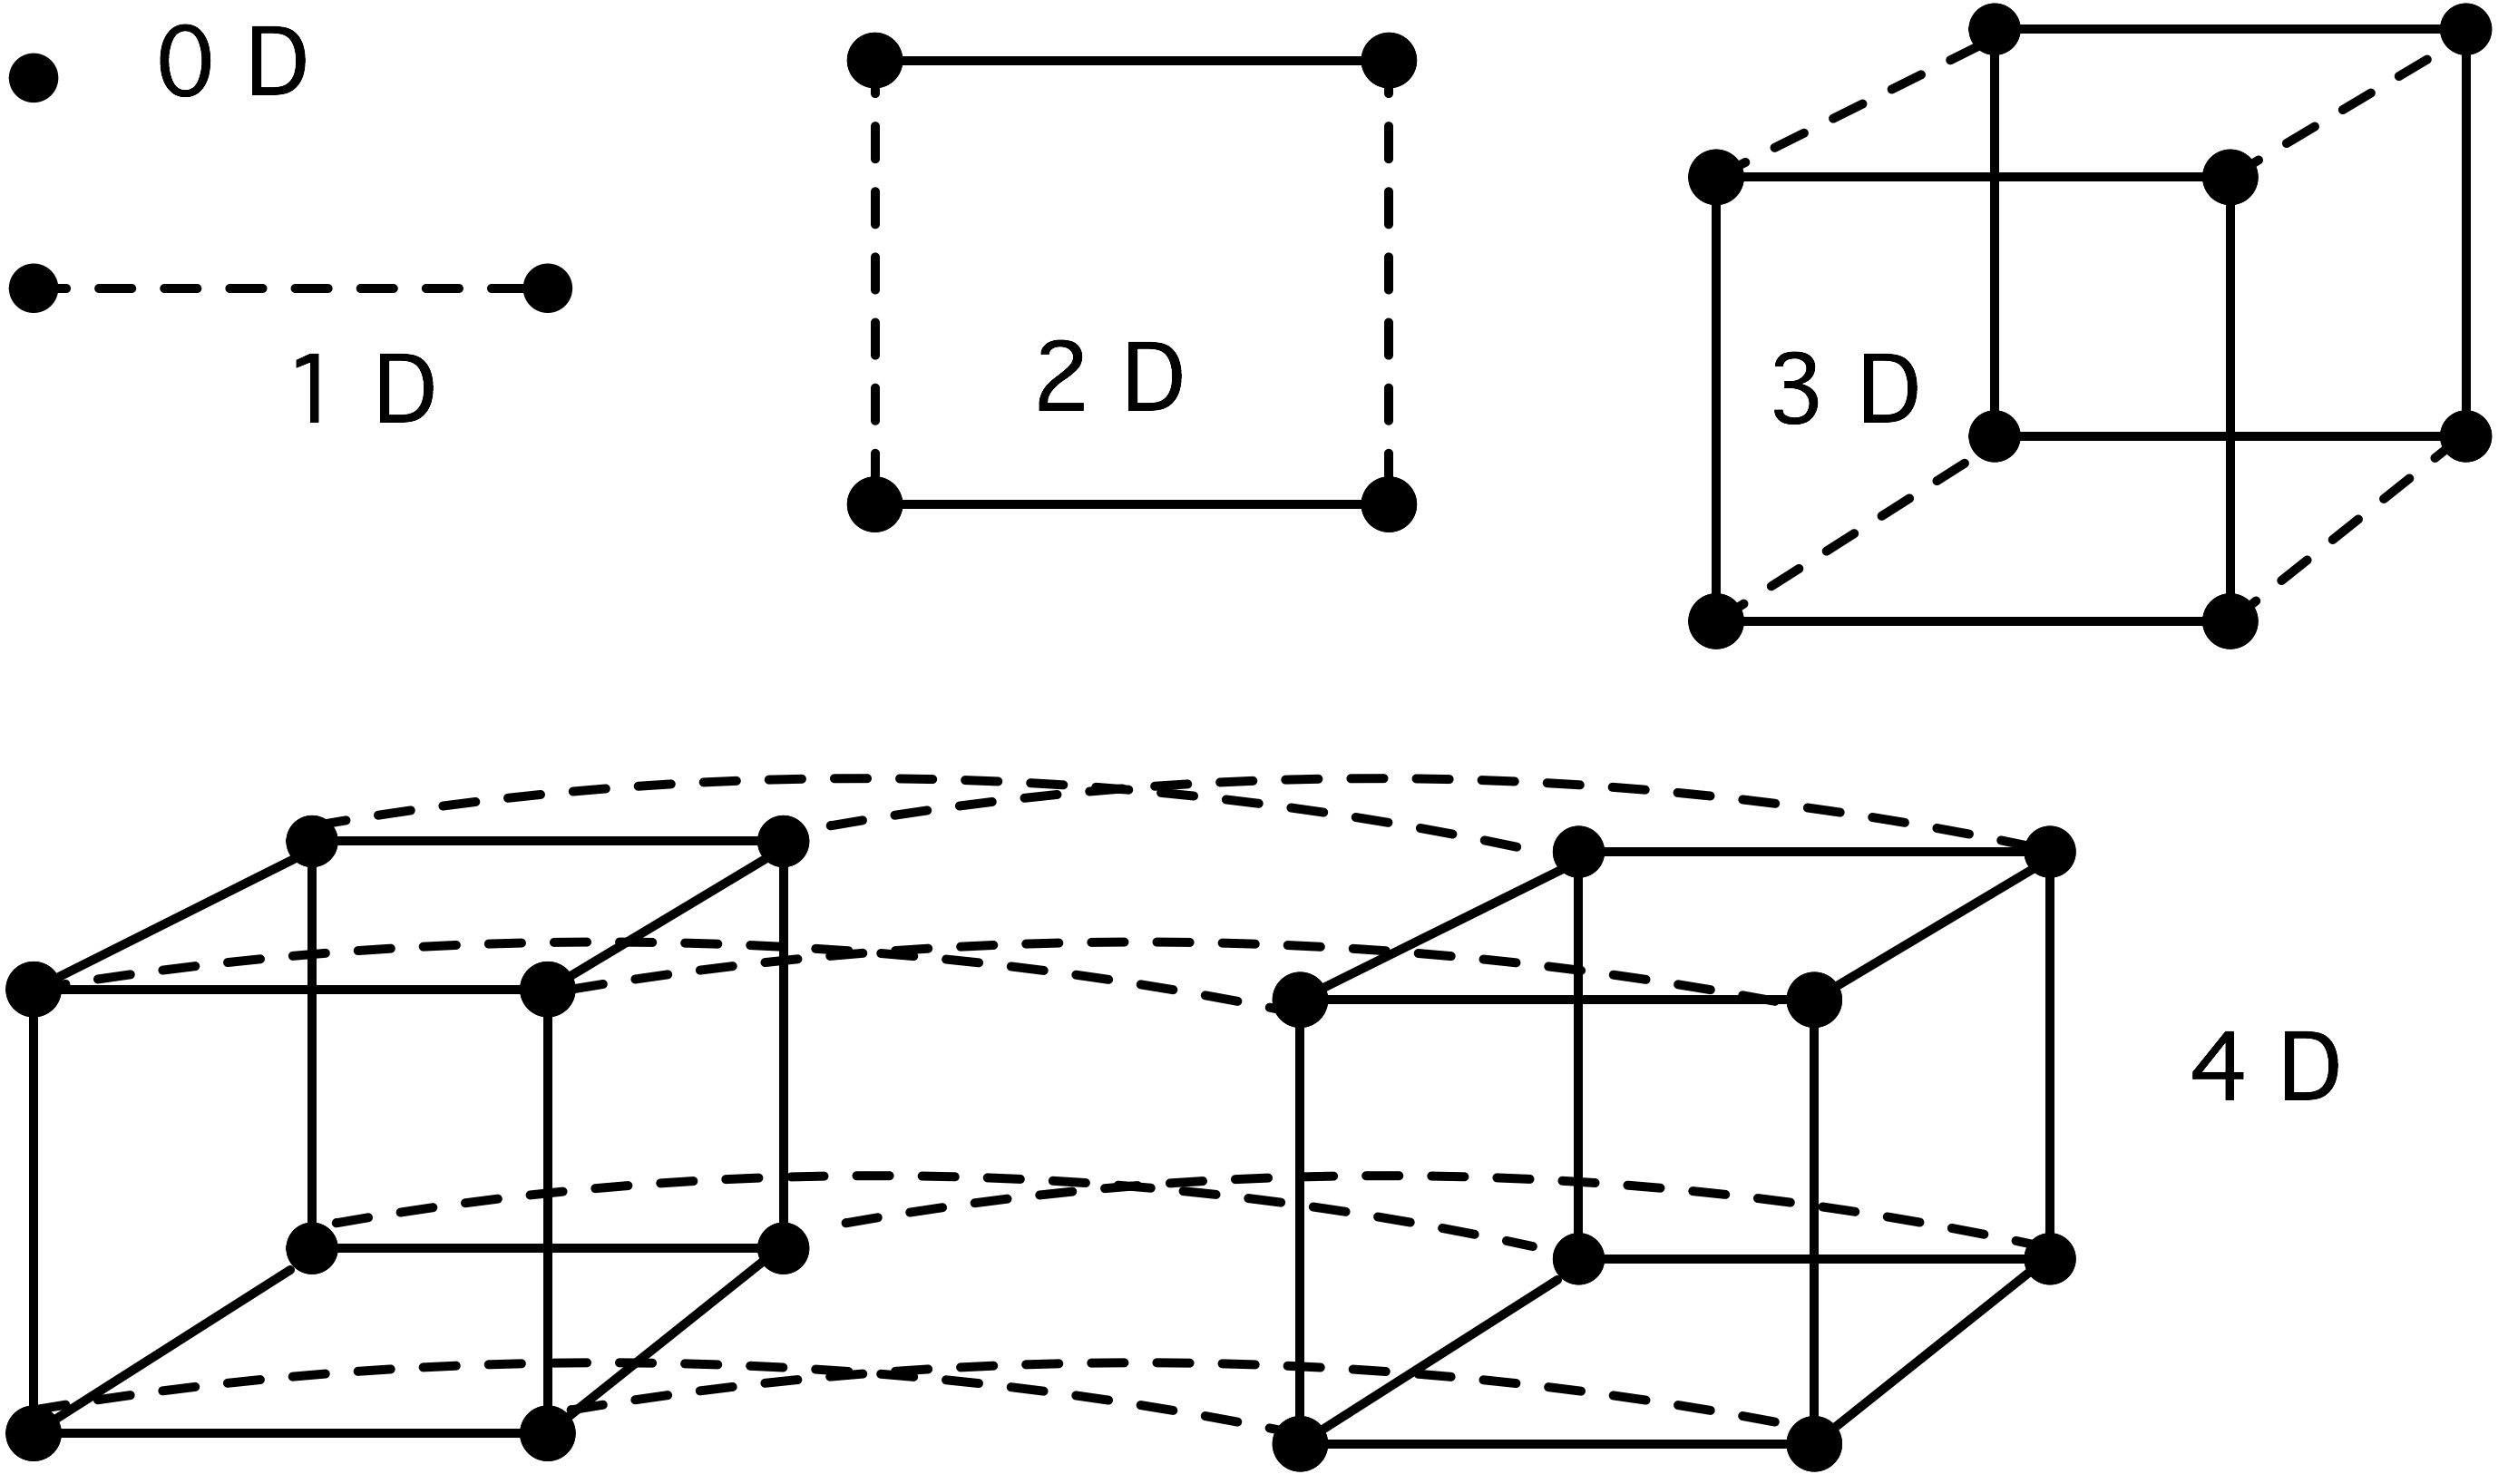
\includegraphics[scale=.1]{hypercubes}
\end{numberedframe}

\begin{numberedframe}{Hypercube numbering}
  Naive numbering:\\
  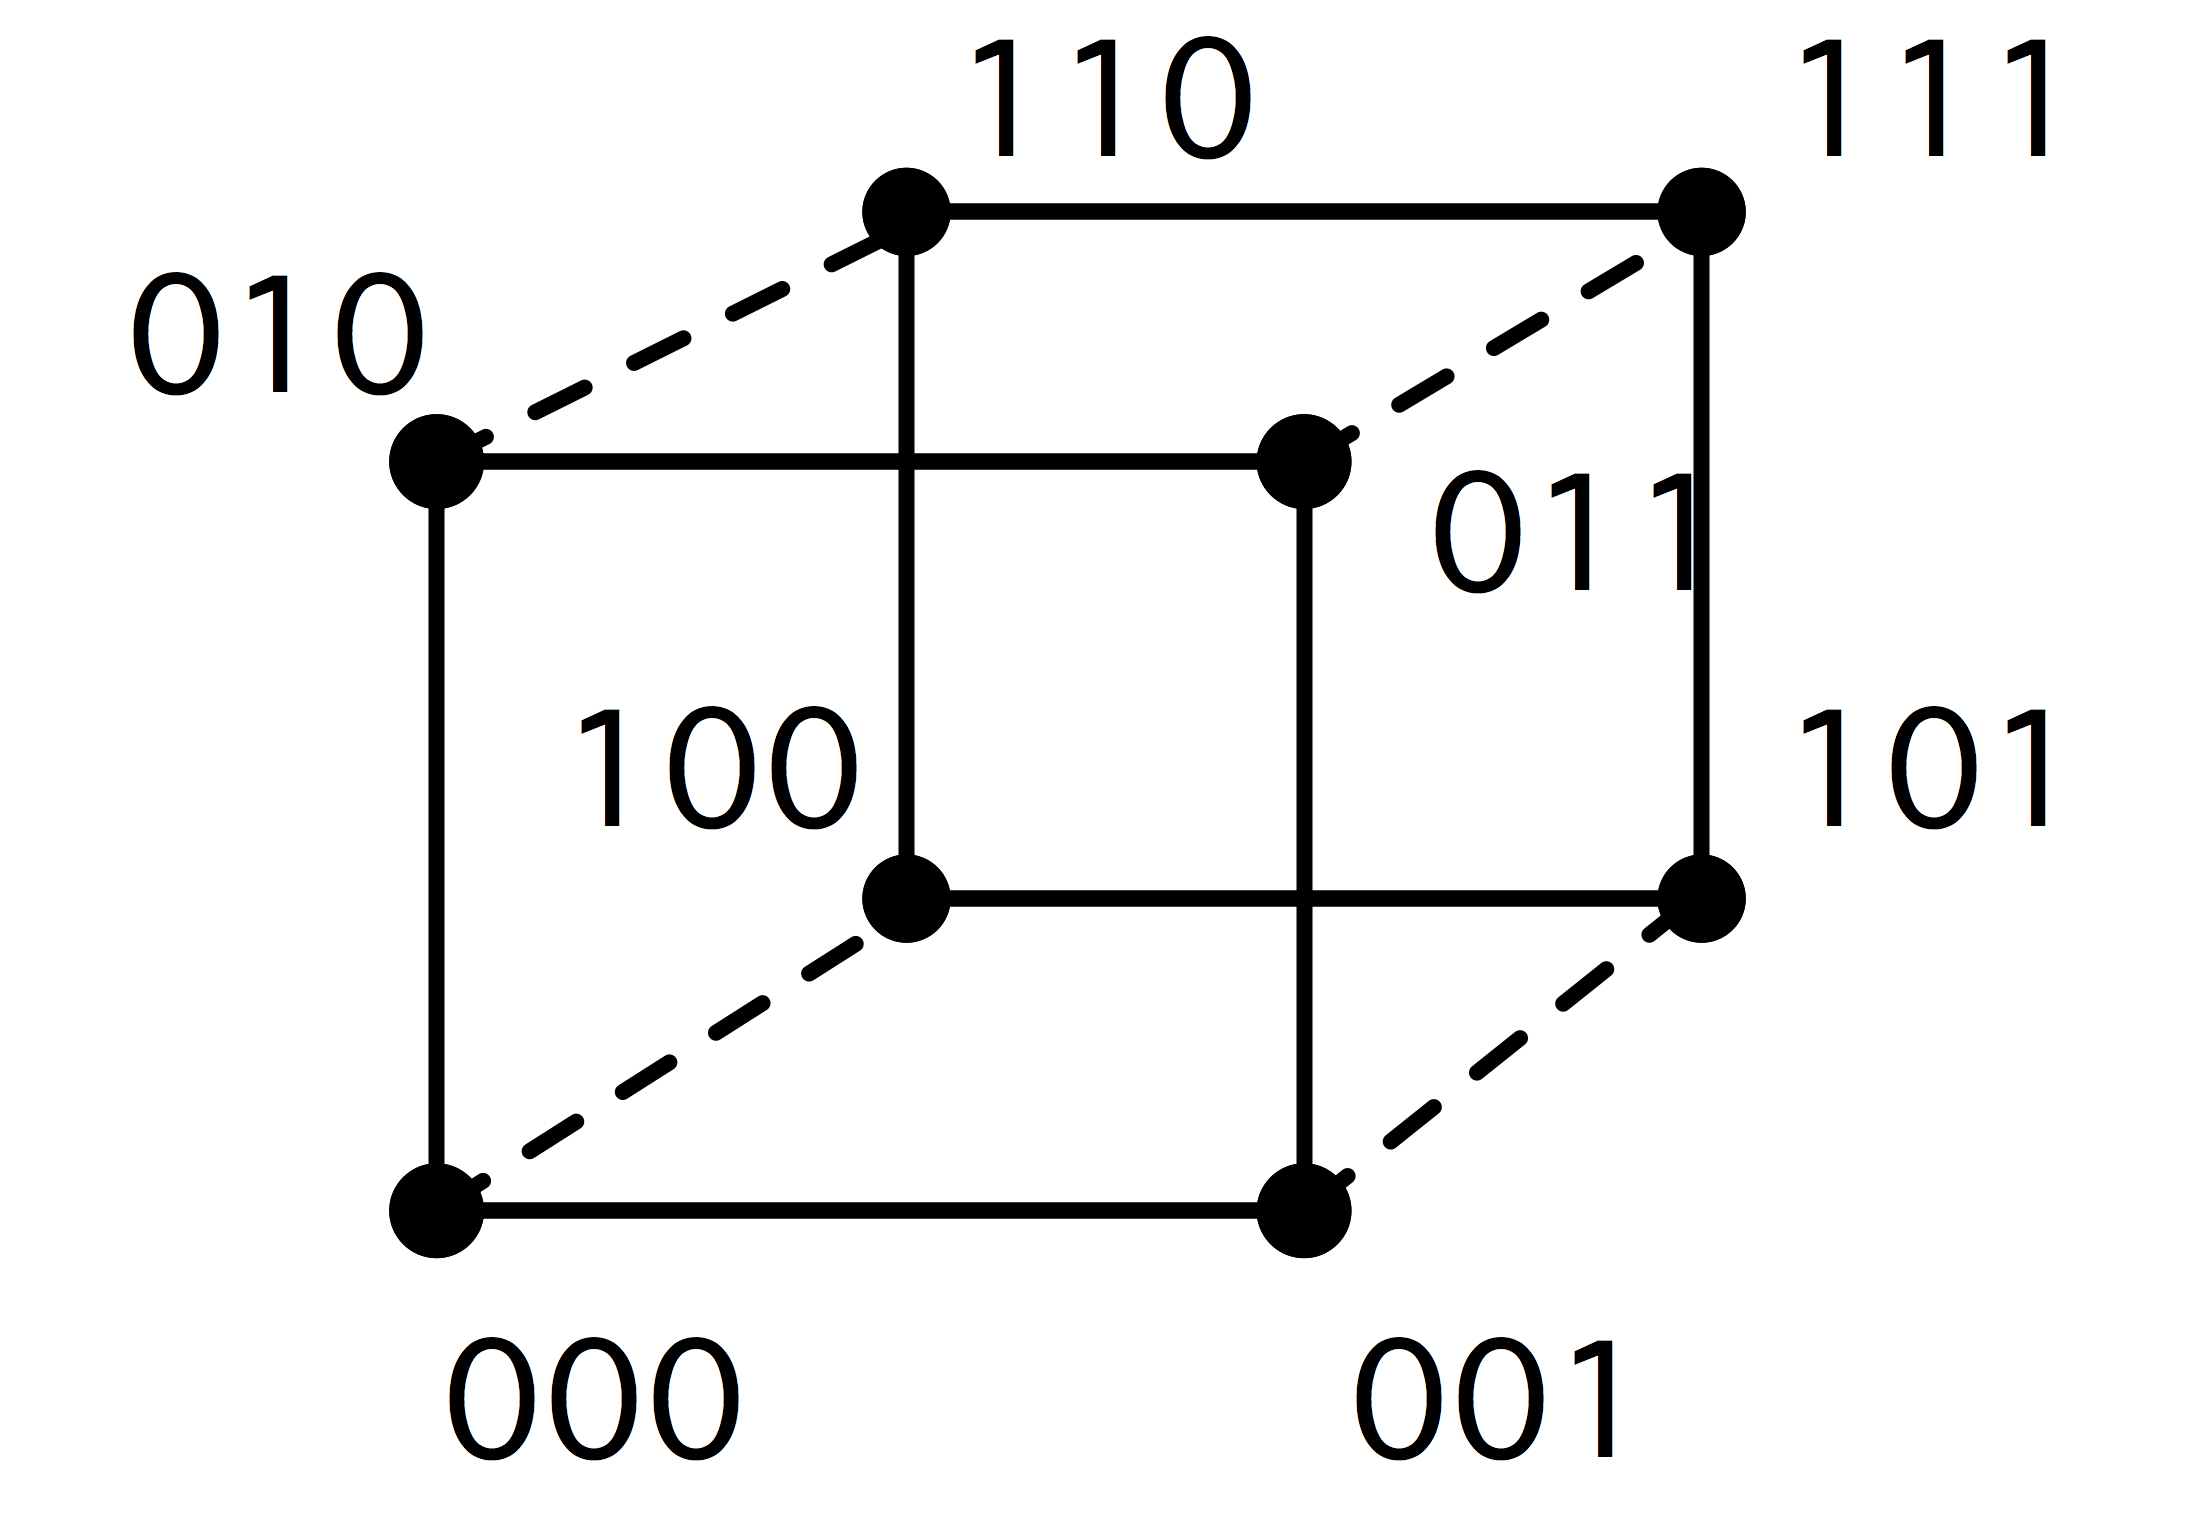
\includegraphics[scale=.1]{hypercubenumber}
\end{numberedframe}

\begin{numberedframe}{Gray codes}
    Embedding linear numbering in hypercube:\\
  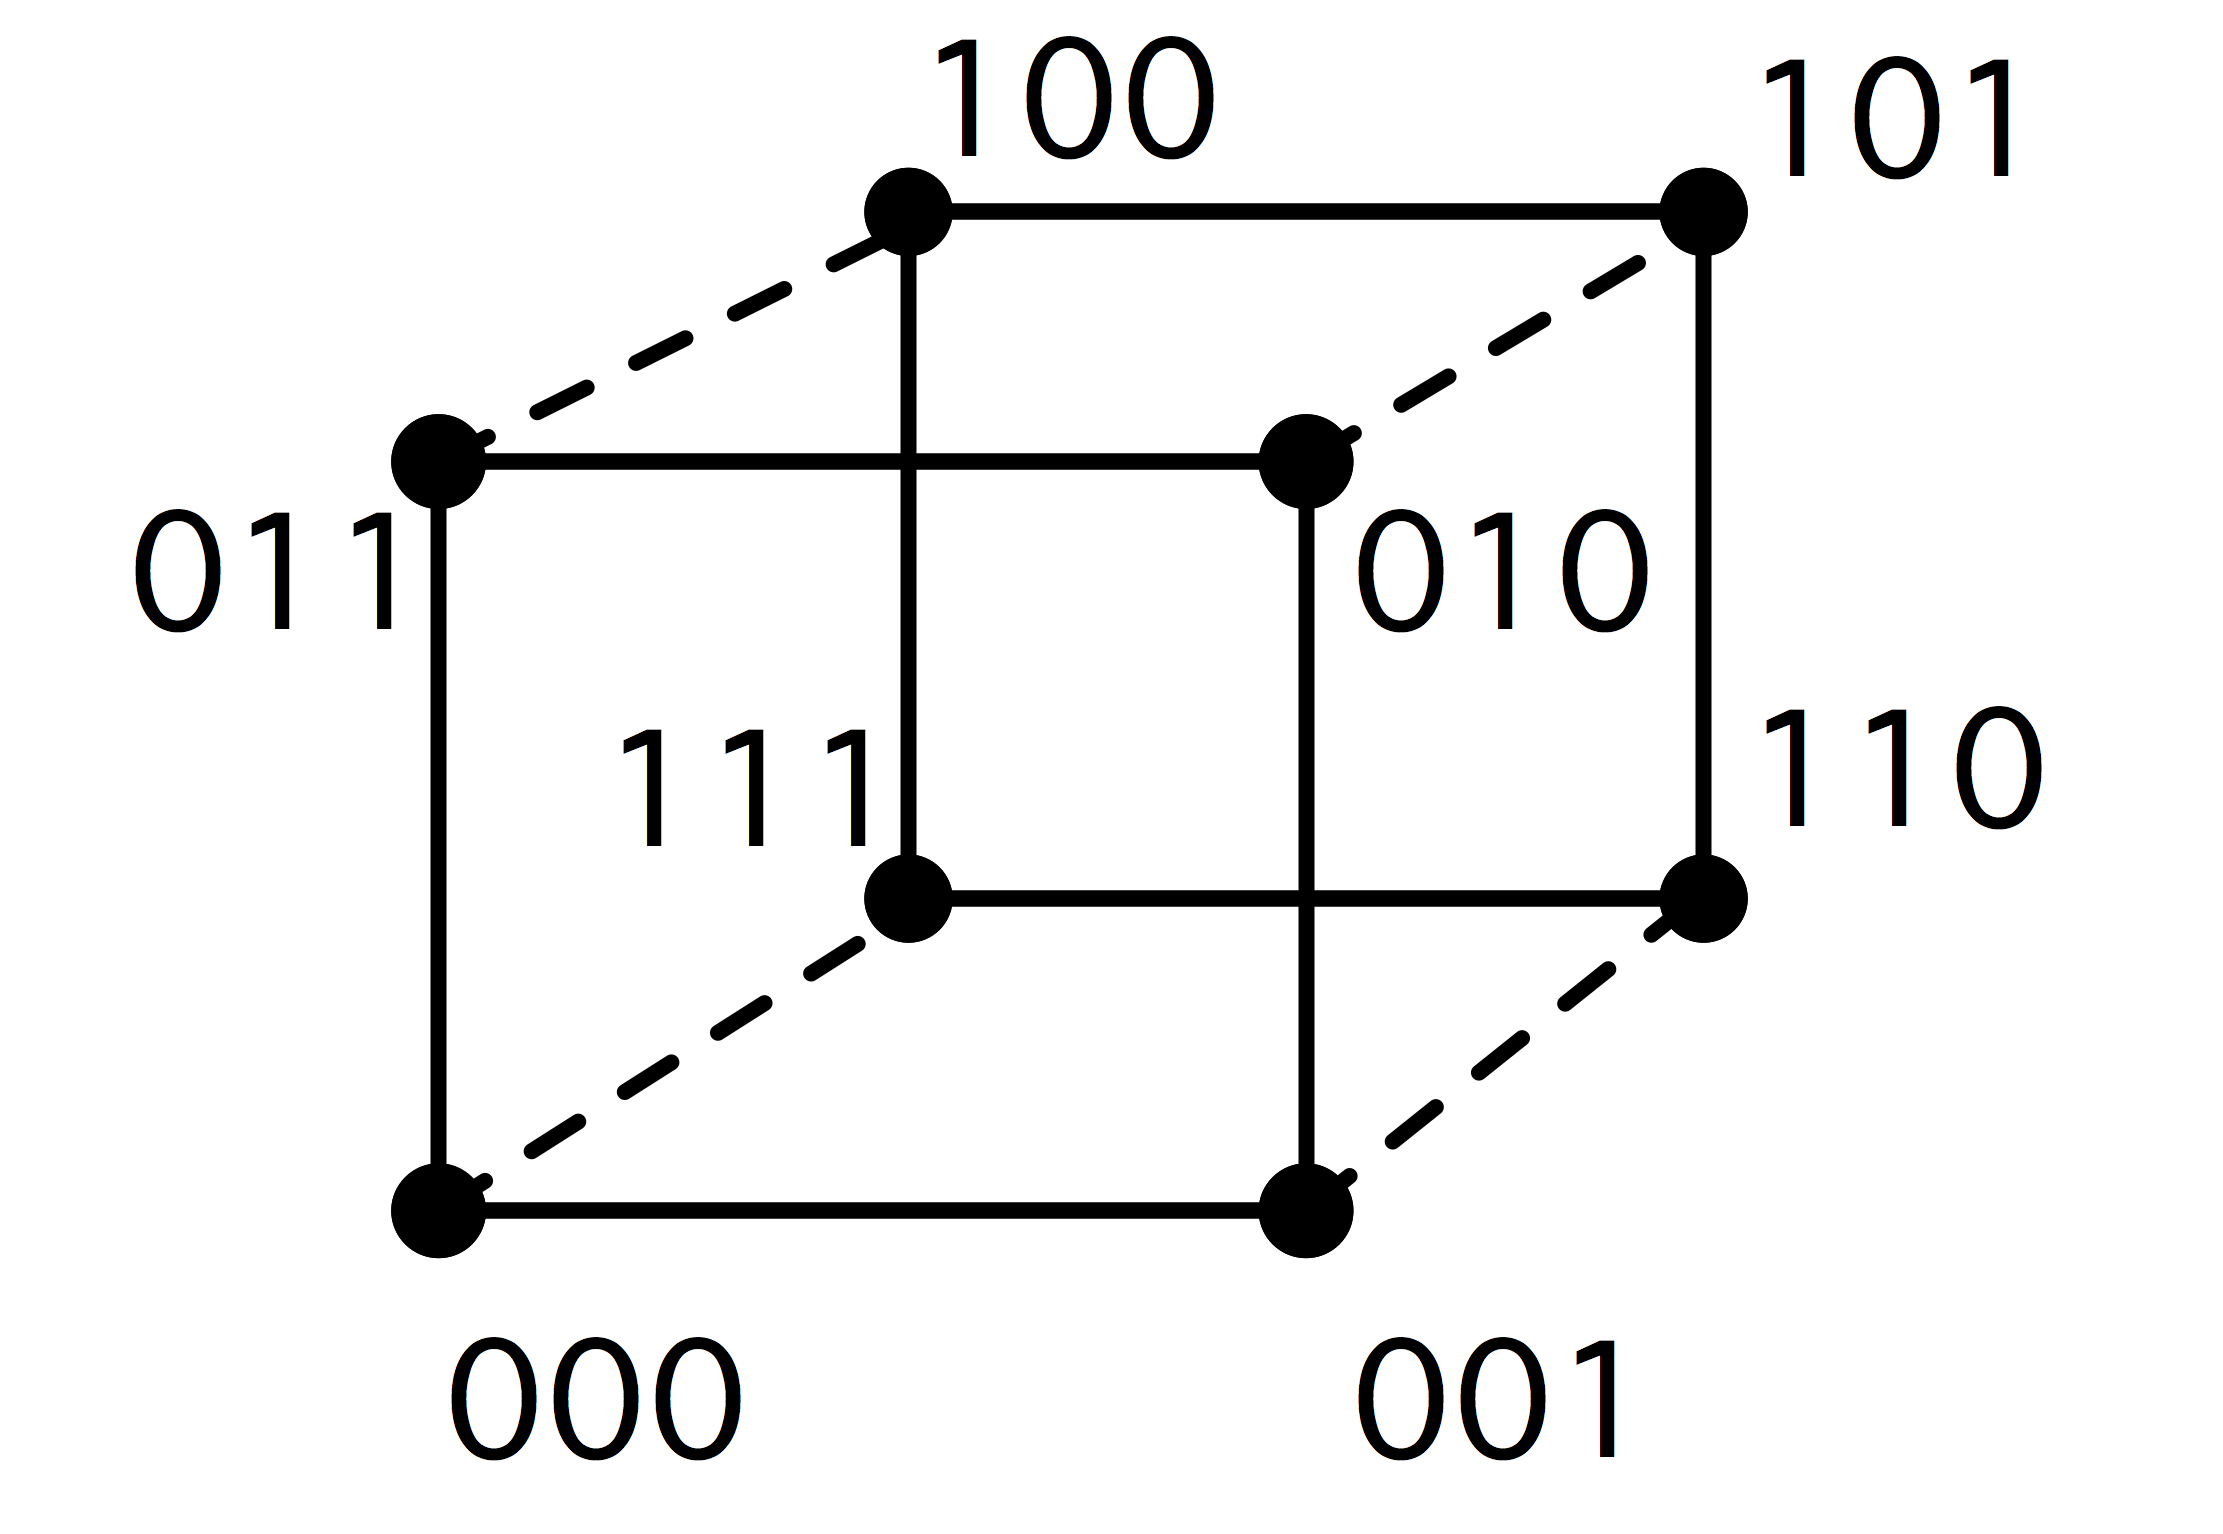
\includegraphics[scale=.081]{hypercubegraynumber}
\end{numberedframe}

\begin{numberedframe}{Binary reflected Gray code}
\small
\hbox{\fbox{1D Gray code}:
$\vcenter{$
\begin{array}{rll}
  \hphantom{1D code and reflection:}&0&1\\
\end{array}$}
$}

\hbox{\fbox{2D Gray code}:
$\vcenter{$
\begin{array}{rccccc}
  \hbox{1D code and reflection:}&0&1&\vdots&1&0\\
  \hbox{append 0 and 1 bit:}&0&0&\vdots&1&1
\end{array}$}
$}

\hbox{\fbox{3D Gray code}:
$\vcenter{$
\begin{array}{rccccccccc}
  \hbox{2D code and reflection:}&0&1&1&0&\vdots&0&1&1&0\\
  &0&0&1&1&\vdots&1&1&0&0\\
  \hbox{append 0 and 1 bit:}&0&0&0&0&\vdots&1&1&1&1
\end{array}$}
$}
\end{numberedframe}

\begin{numberedframe}{Switching networks}
  \begin{itemize}
  \item Solution to all-to-all connection
  \item (Real all-to-all too expensive)
  \item Typically layered
  \item Switching elements: easy to extend
  \end{itemize}
\end{numberedframe}

\begin{numberedframe}{Cross bar}
    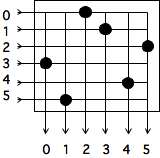
\includegraphics[scale=.7]{crossbar}\\
    Advantage: non-blocking\\
    Disadvantage: cost
\end{numberedframe}

\begin{numberedframe}{Butterfly exchange}
  Process to segmented pool of memory, or between processors with private memory:

    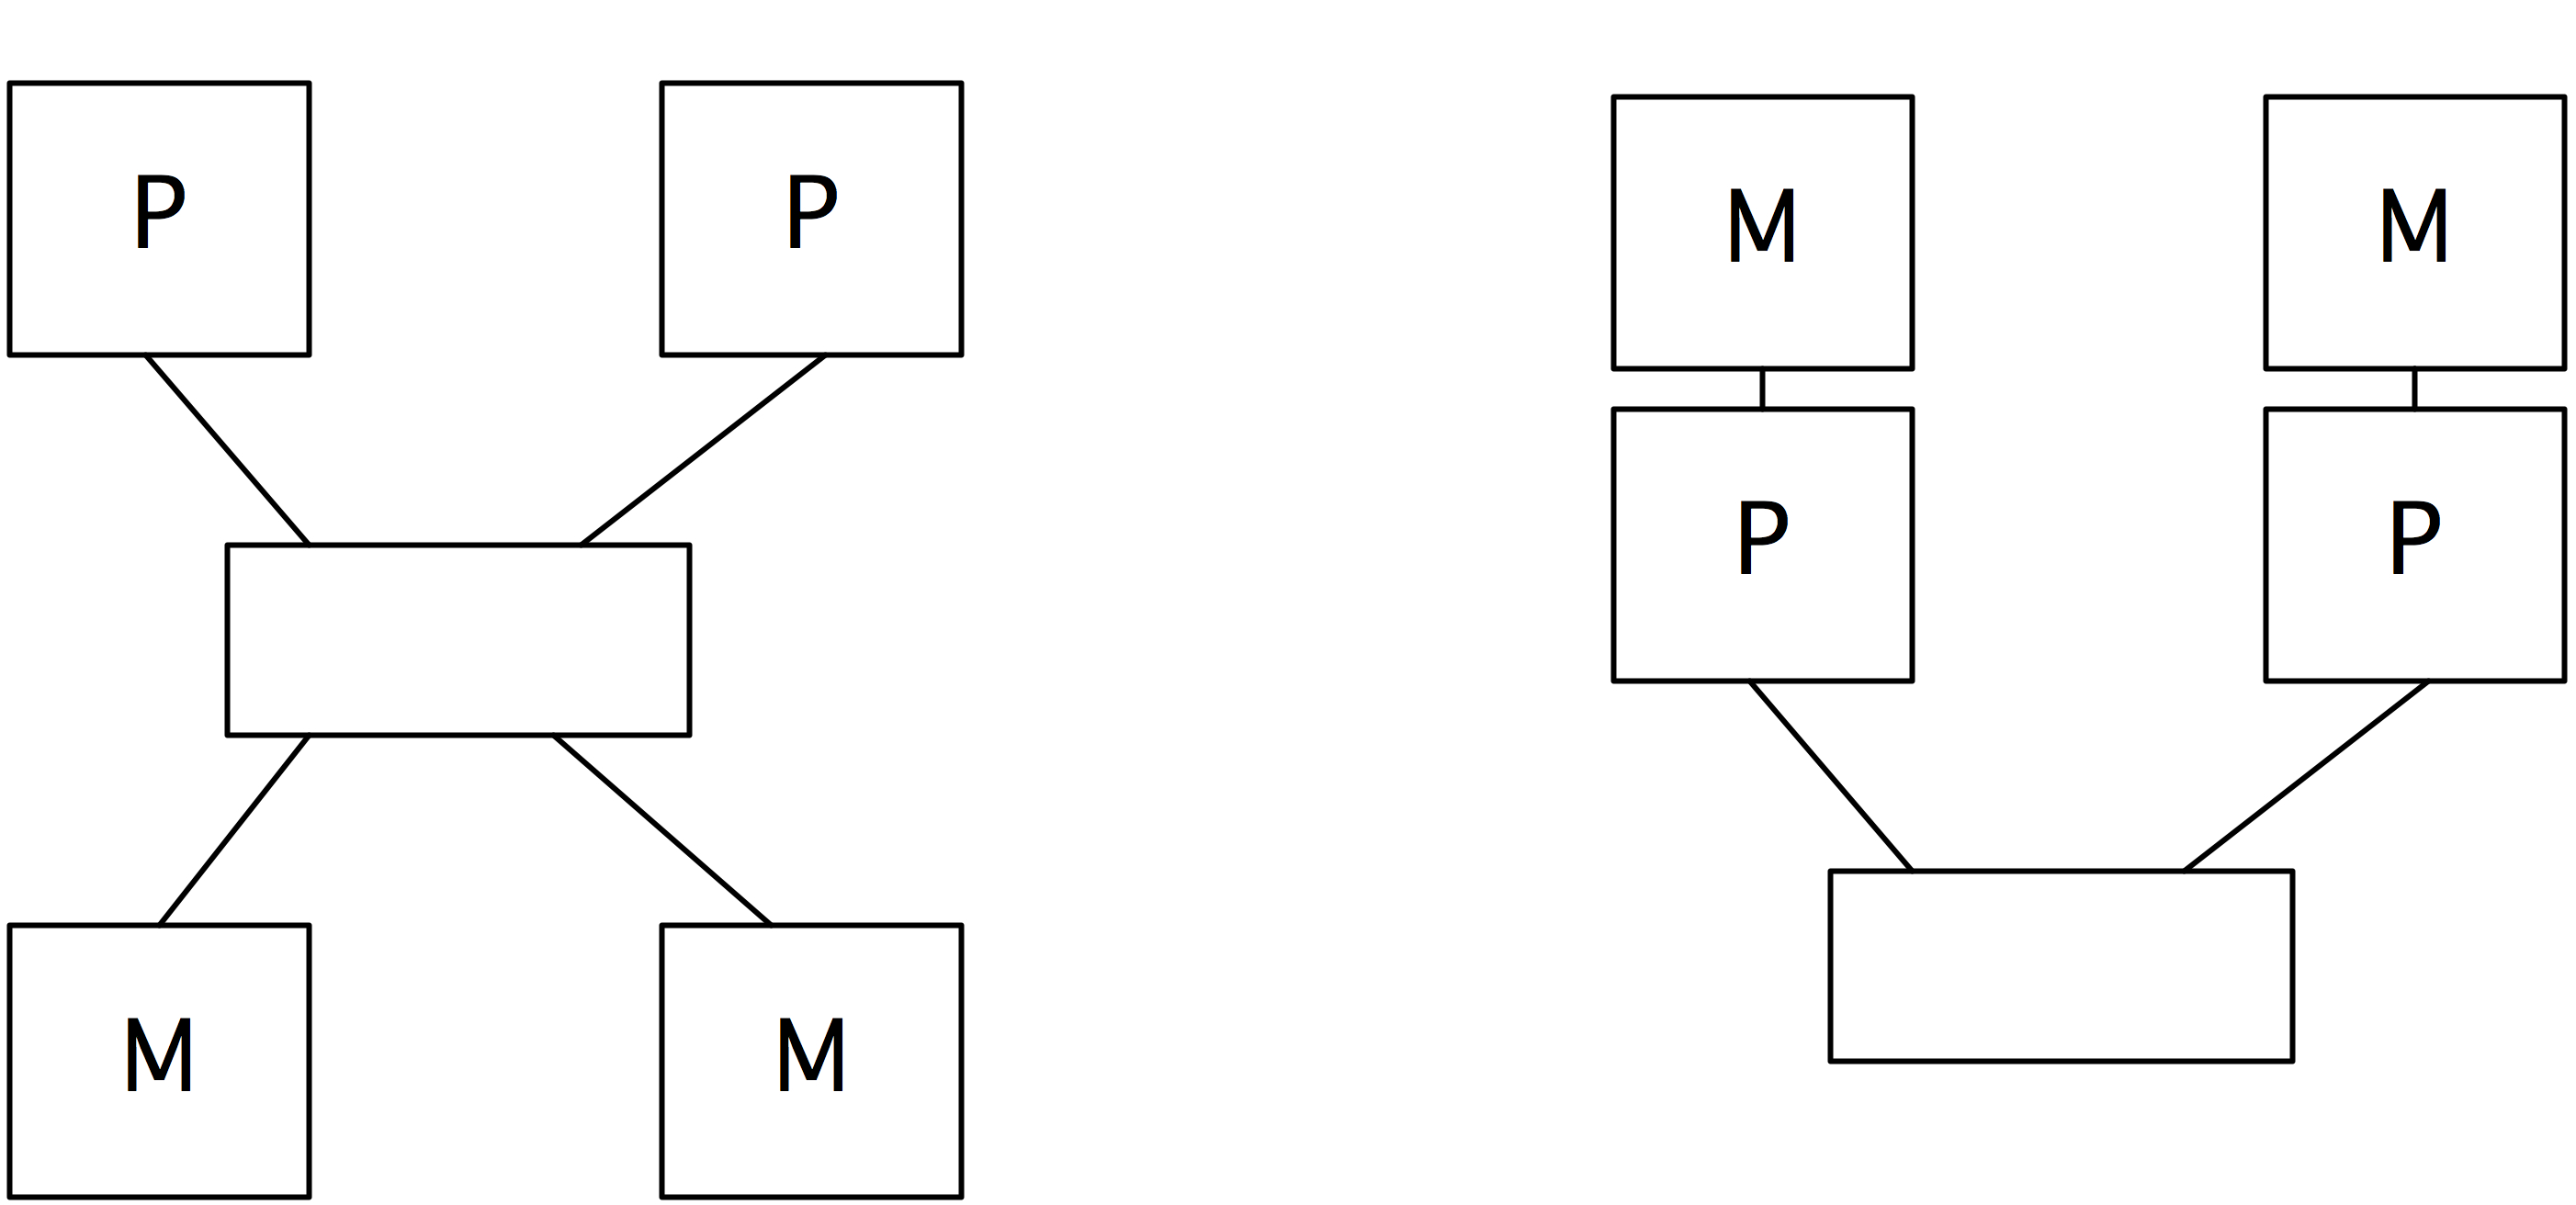
\includegraphics[scale=.08]{butterfly1}
\end{numberedframe}

\begin{numberedframe}{Building up butterflies}
      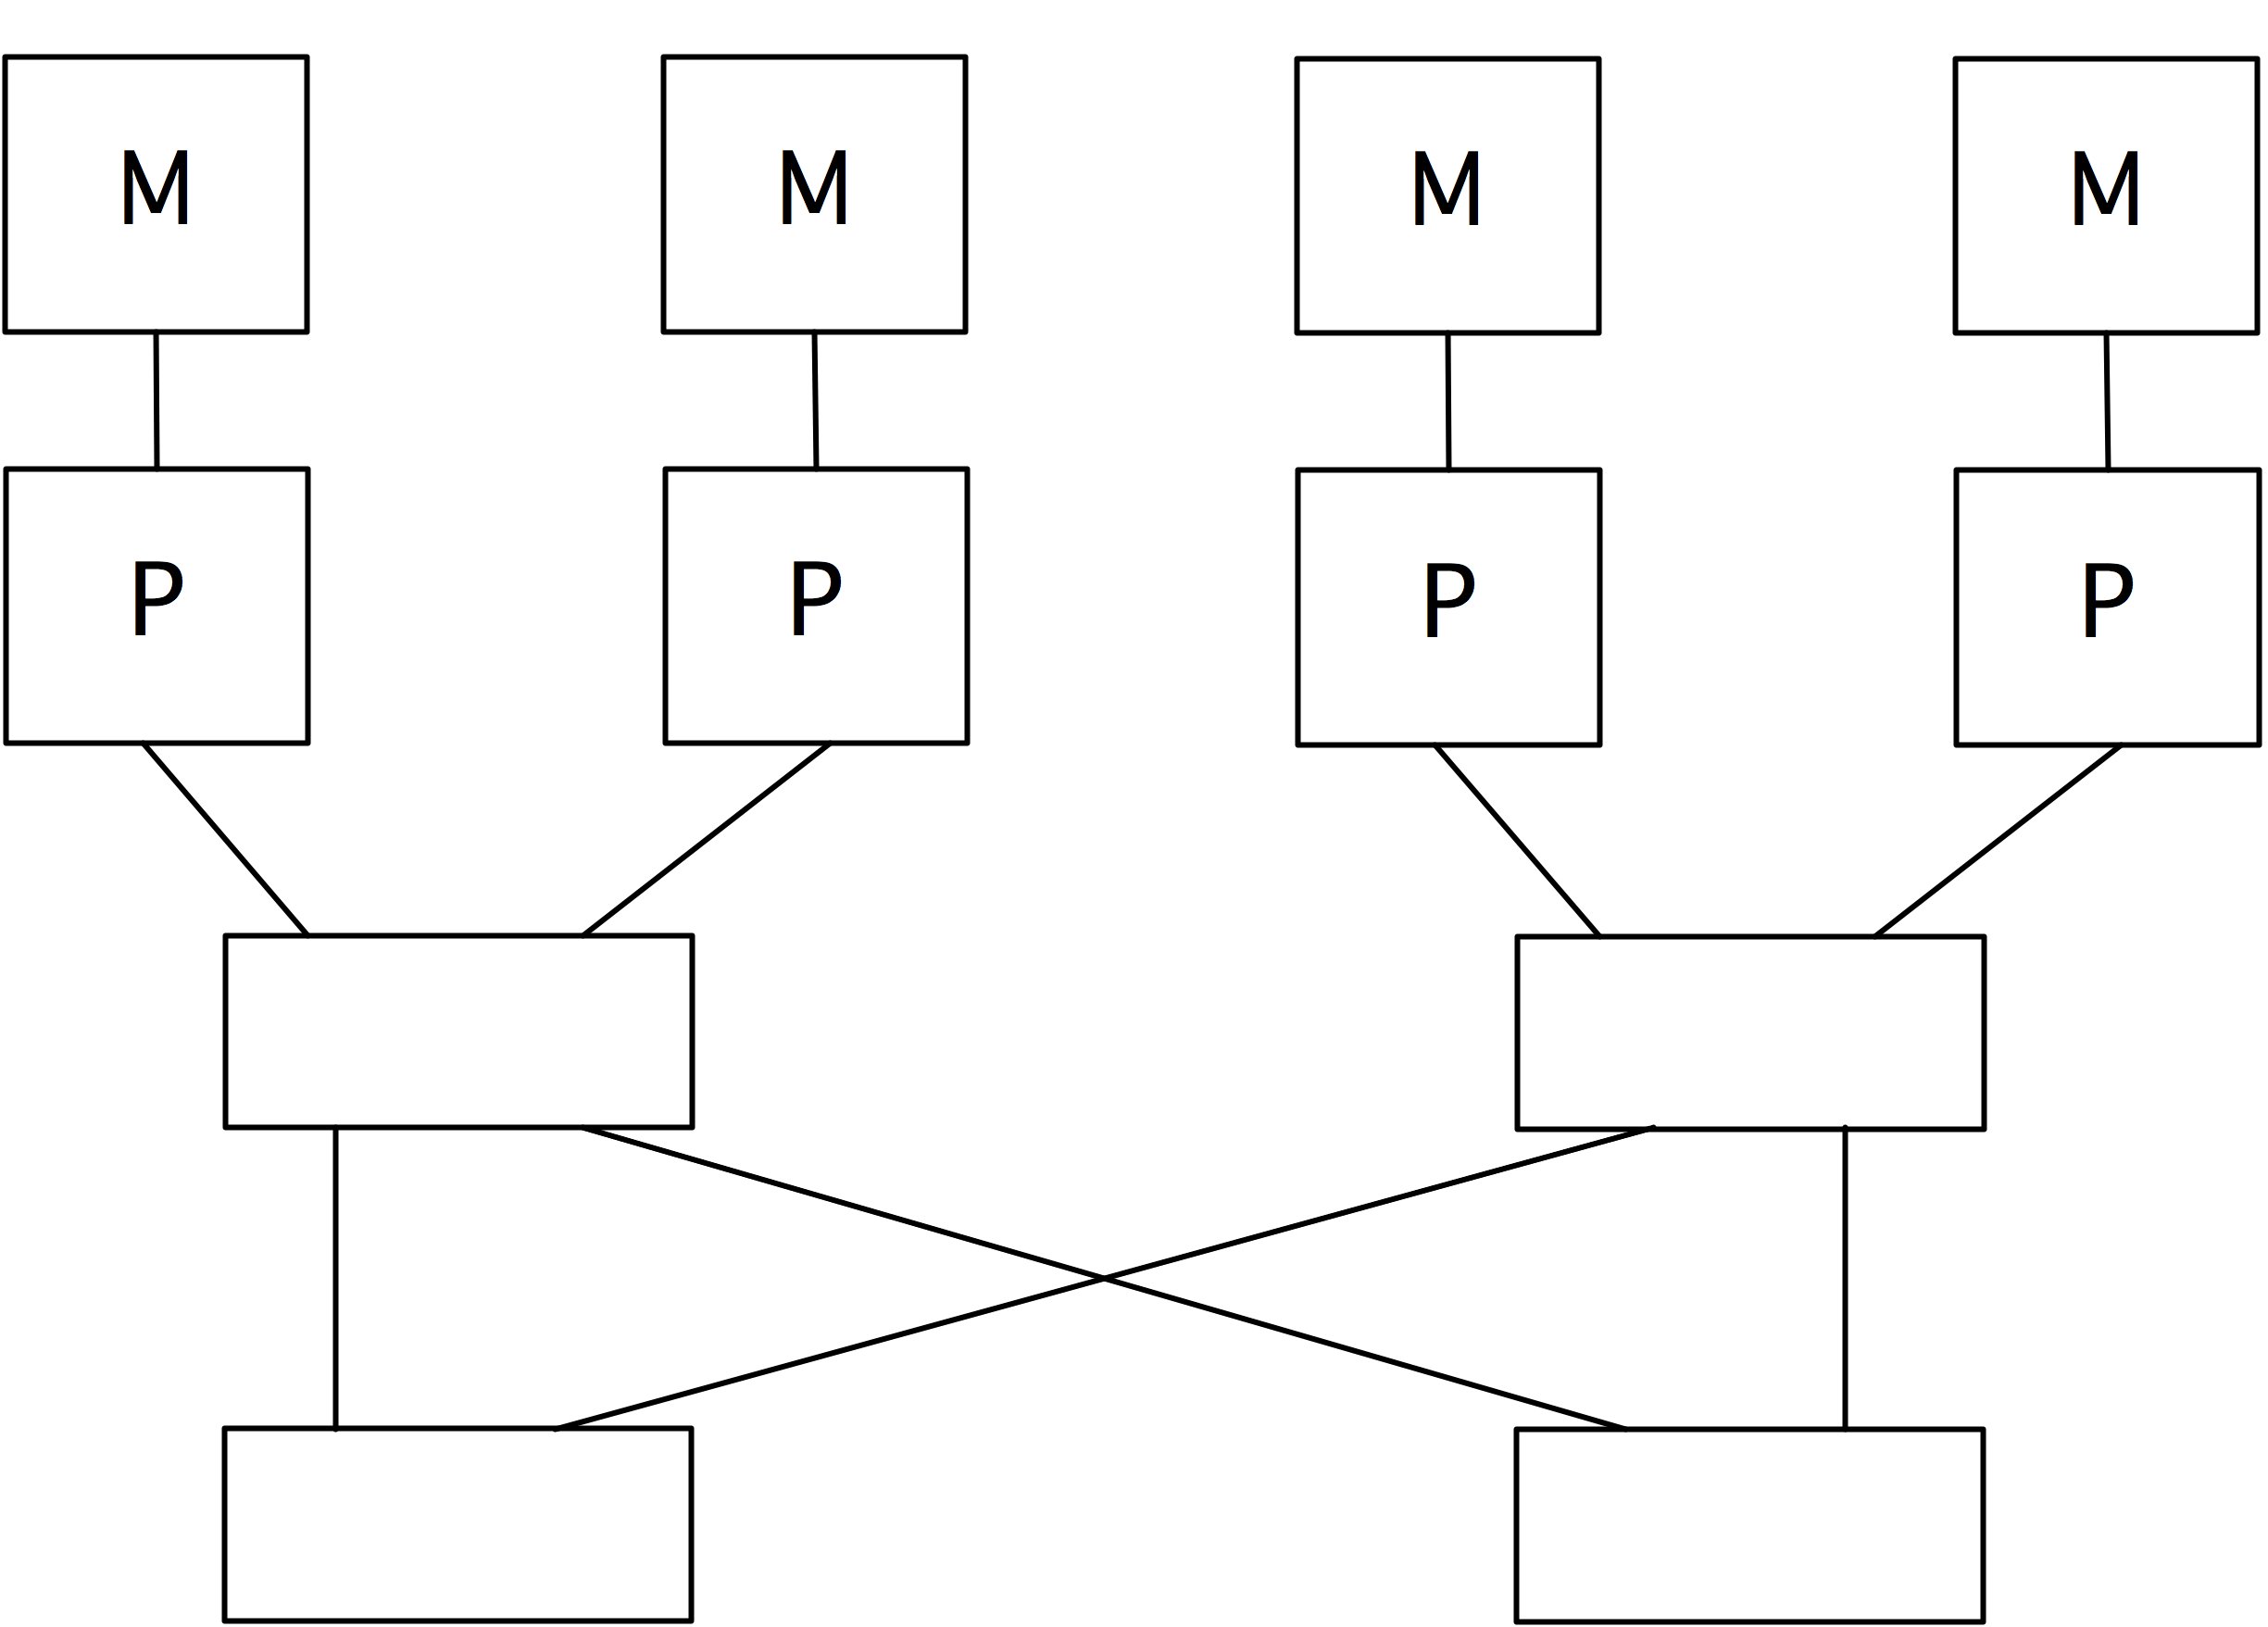
\includegraphics[scale=.08]{butterfly2}
\end{numberedframe}

\begin{numberedframe}{Uniform memory access}
  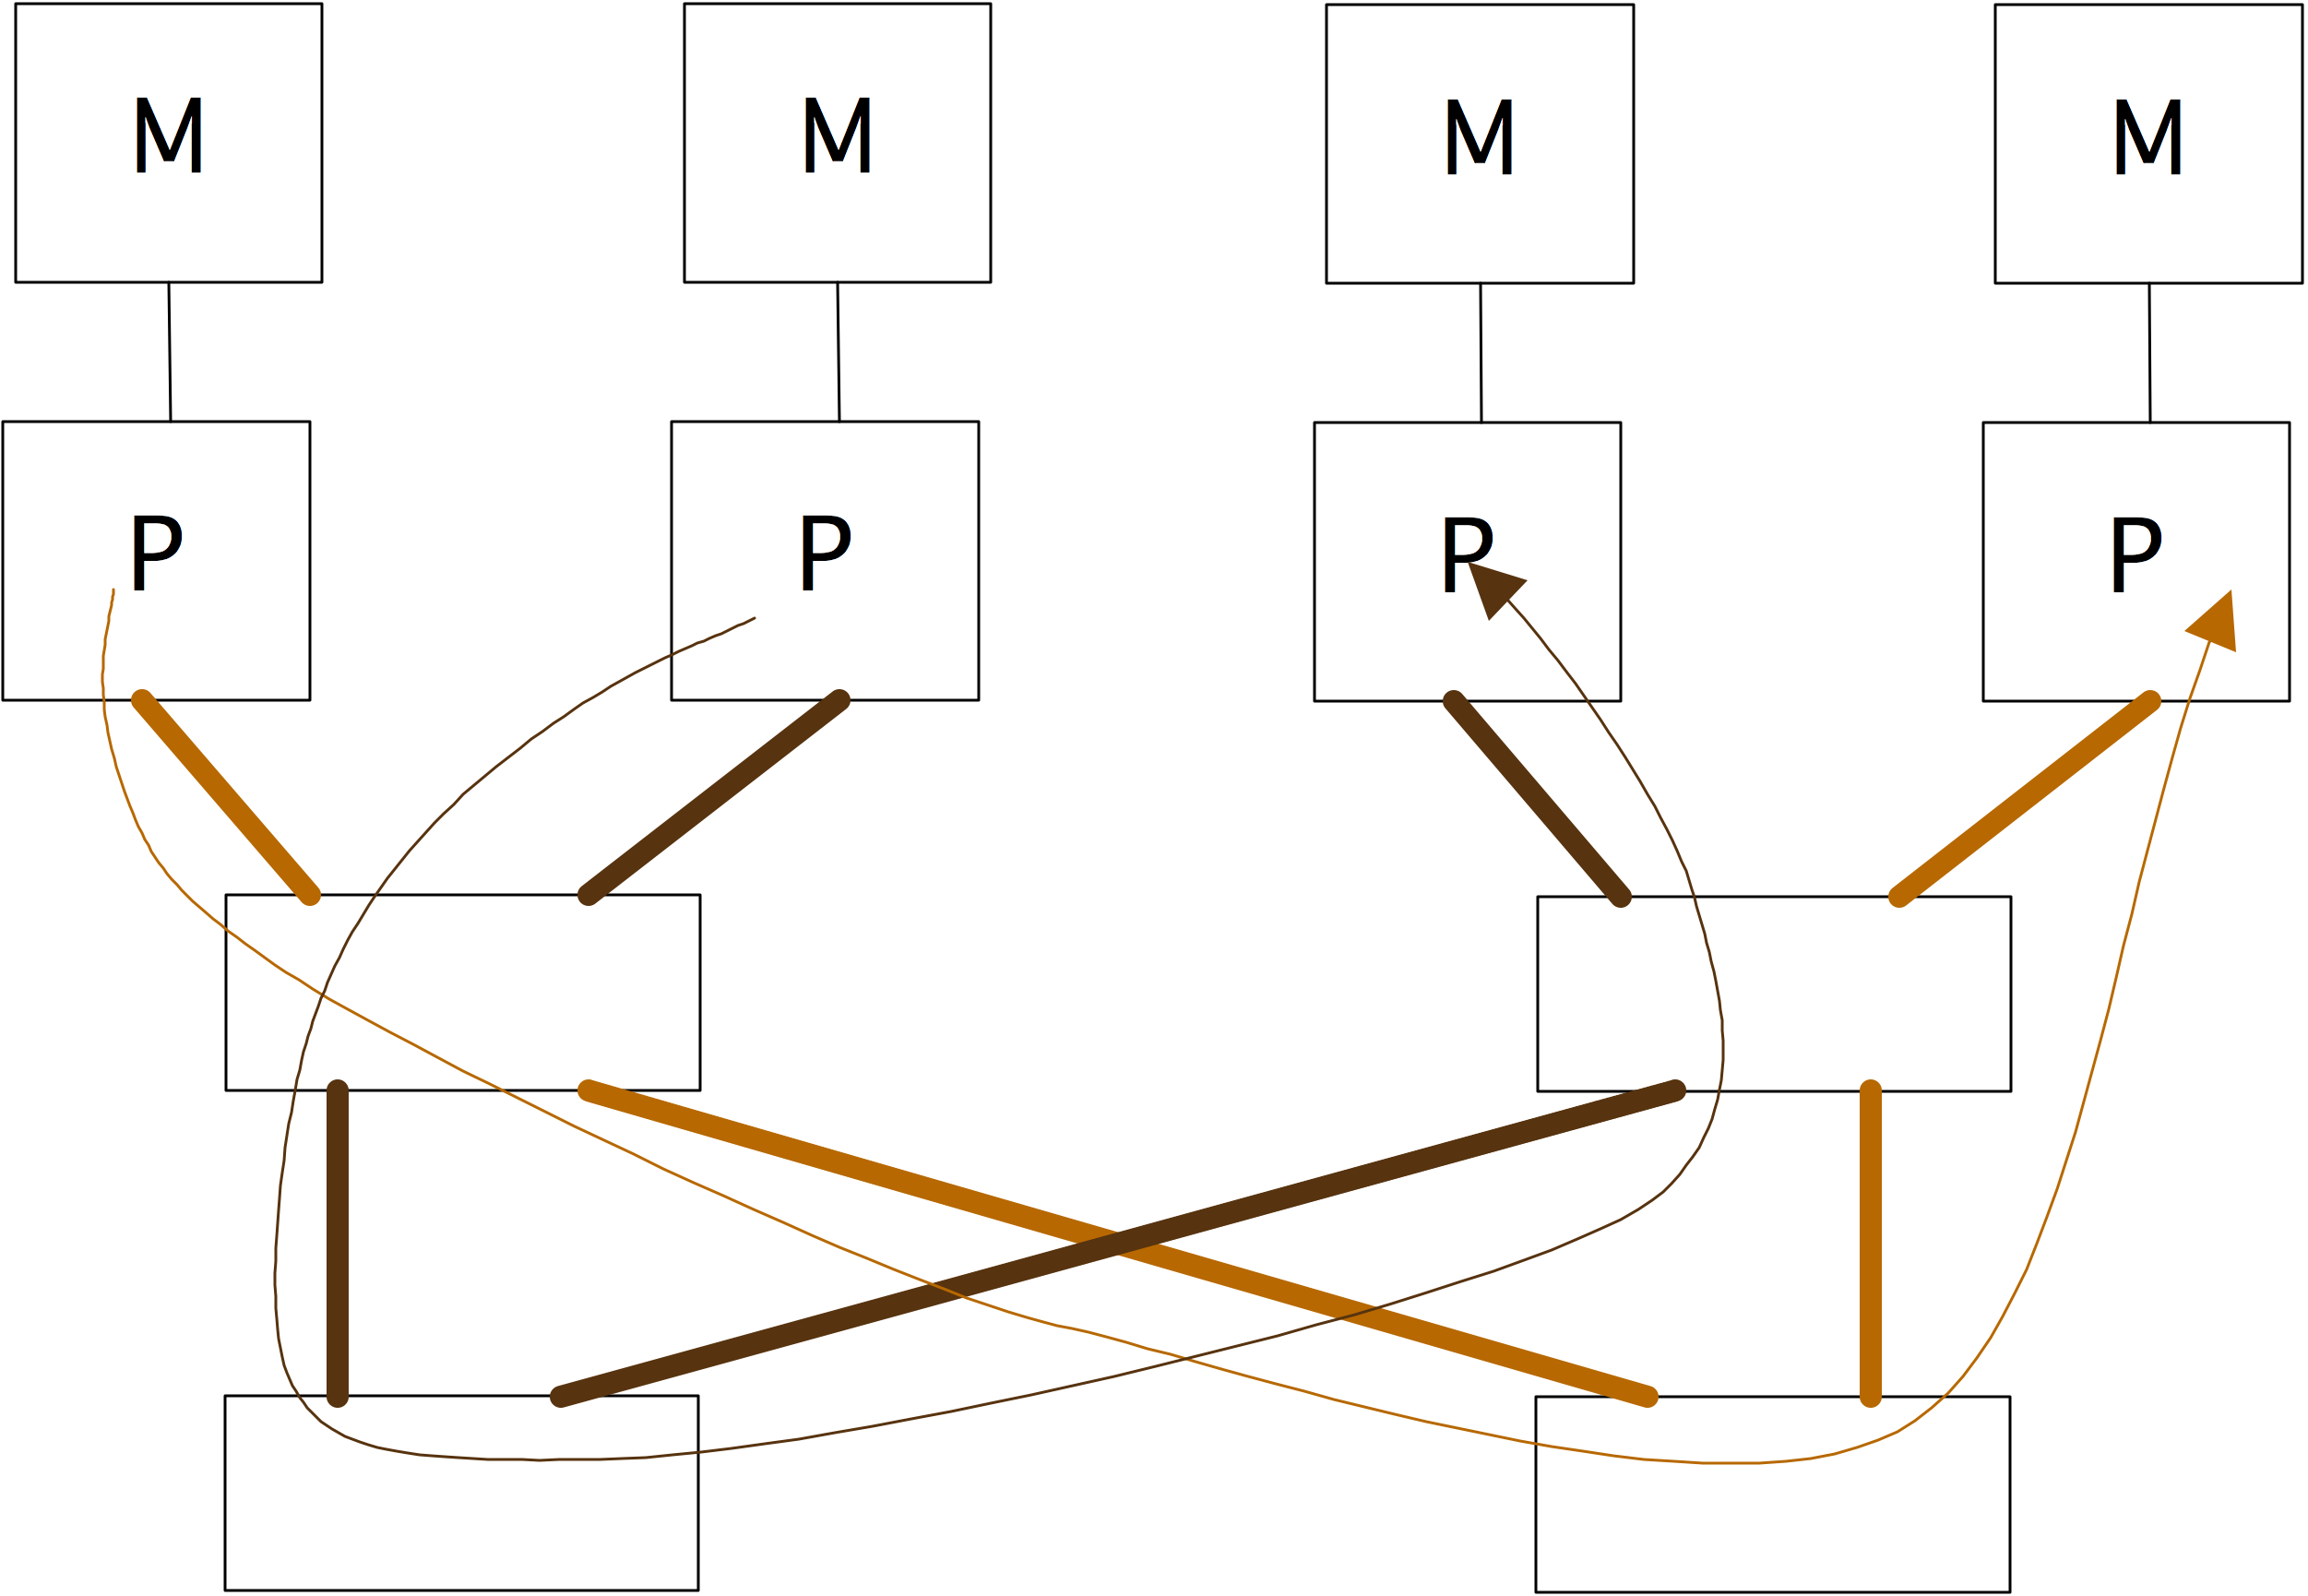
\includegraphics[scale=.1]{butterfly3}
  
  Contention possible
\end{numberedframe}

\begin{numberedframe}{Route calculation}
  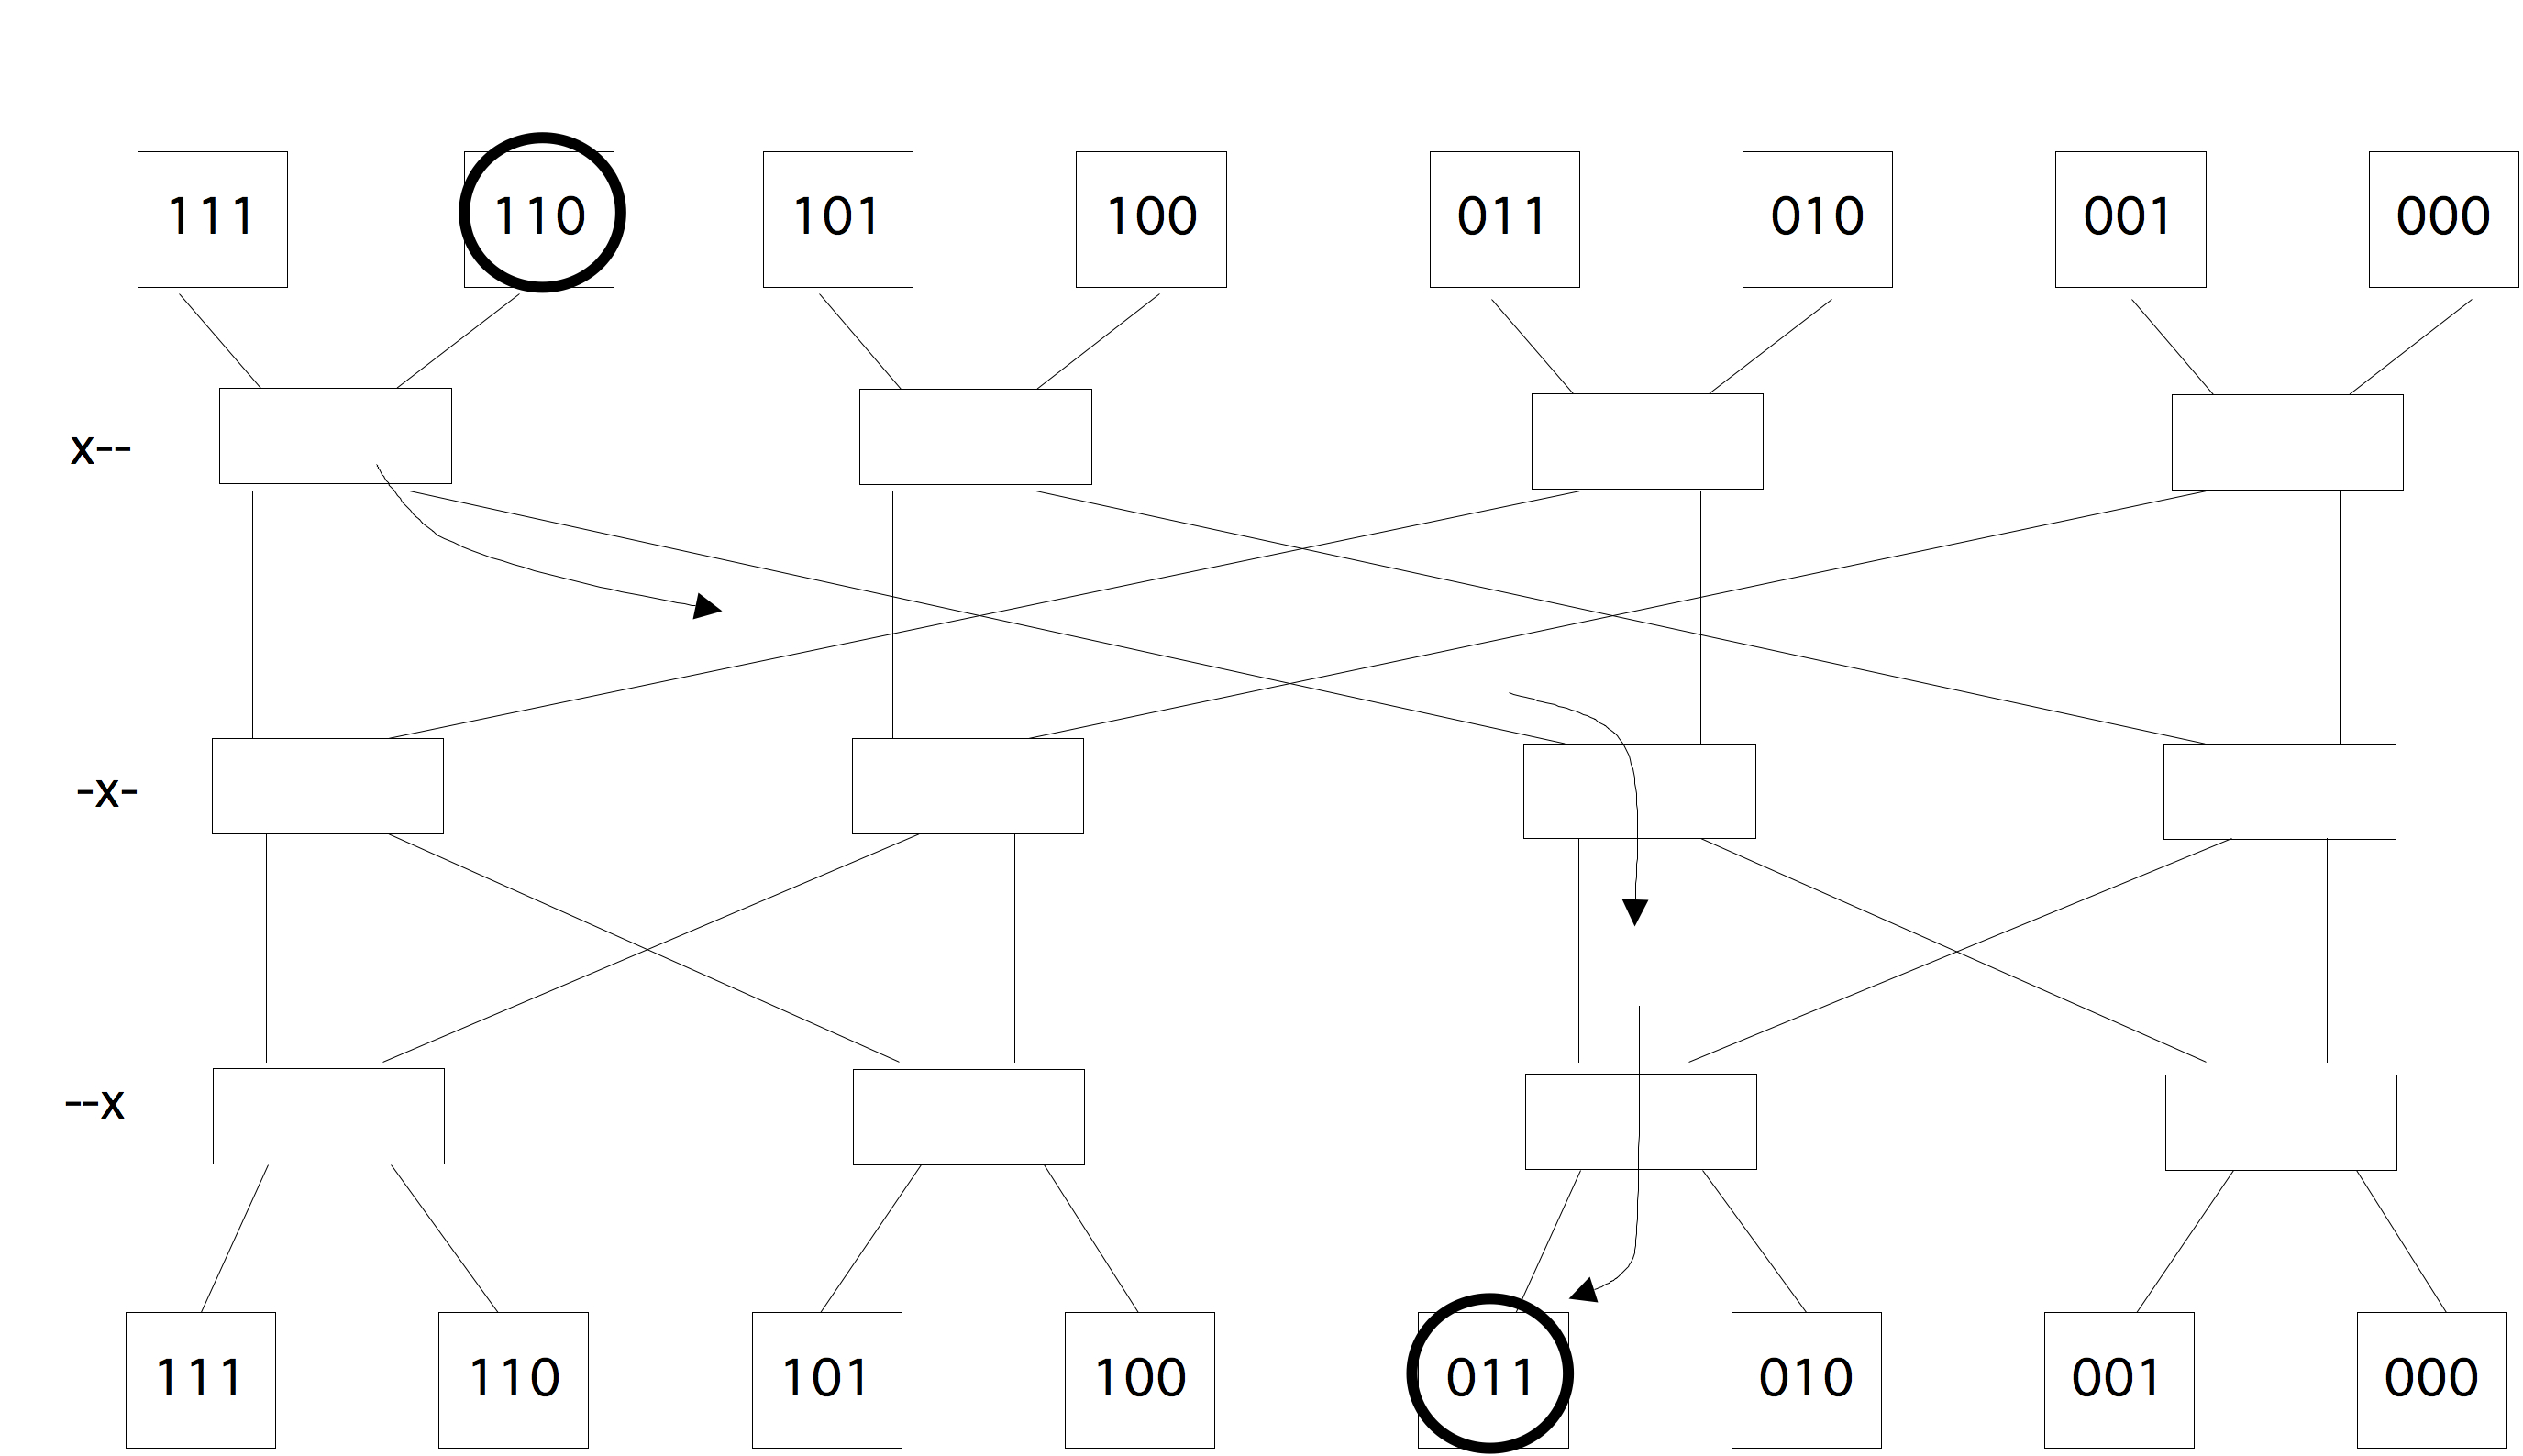
\includegraphics[scale=.13]{butterfly-route}
\end{numberedframe}

\begin{numberedframe}{Fat Tree}
\hbox{%
  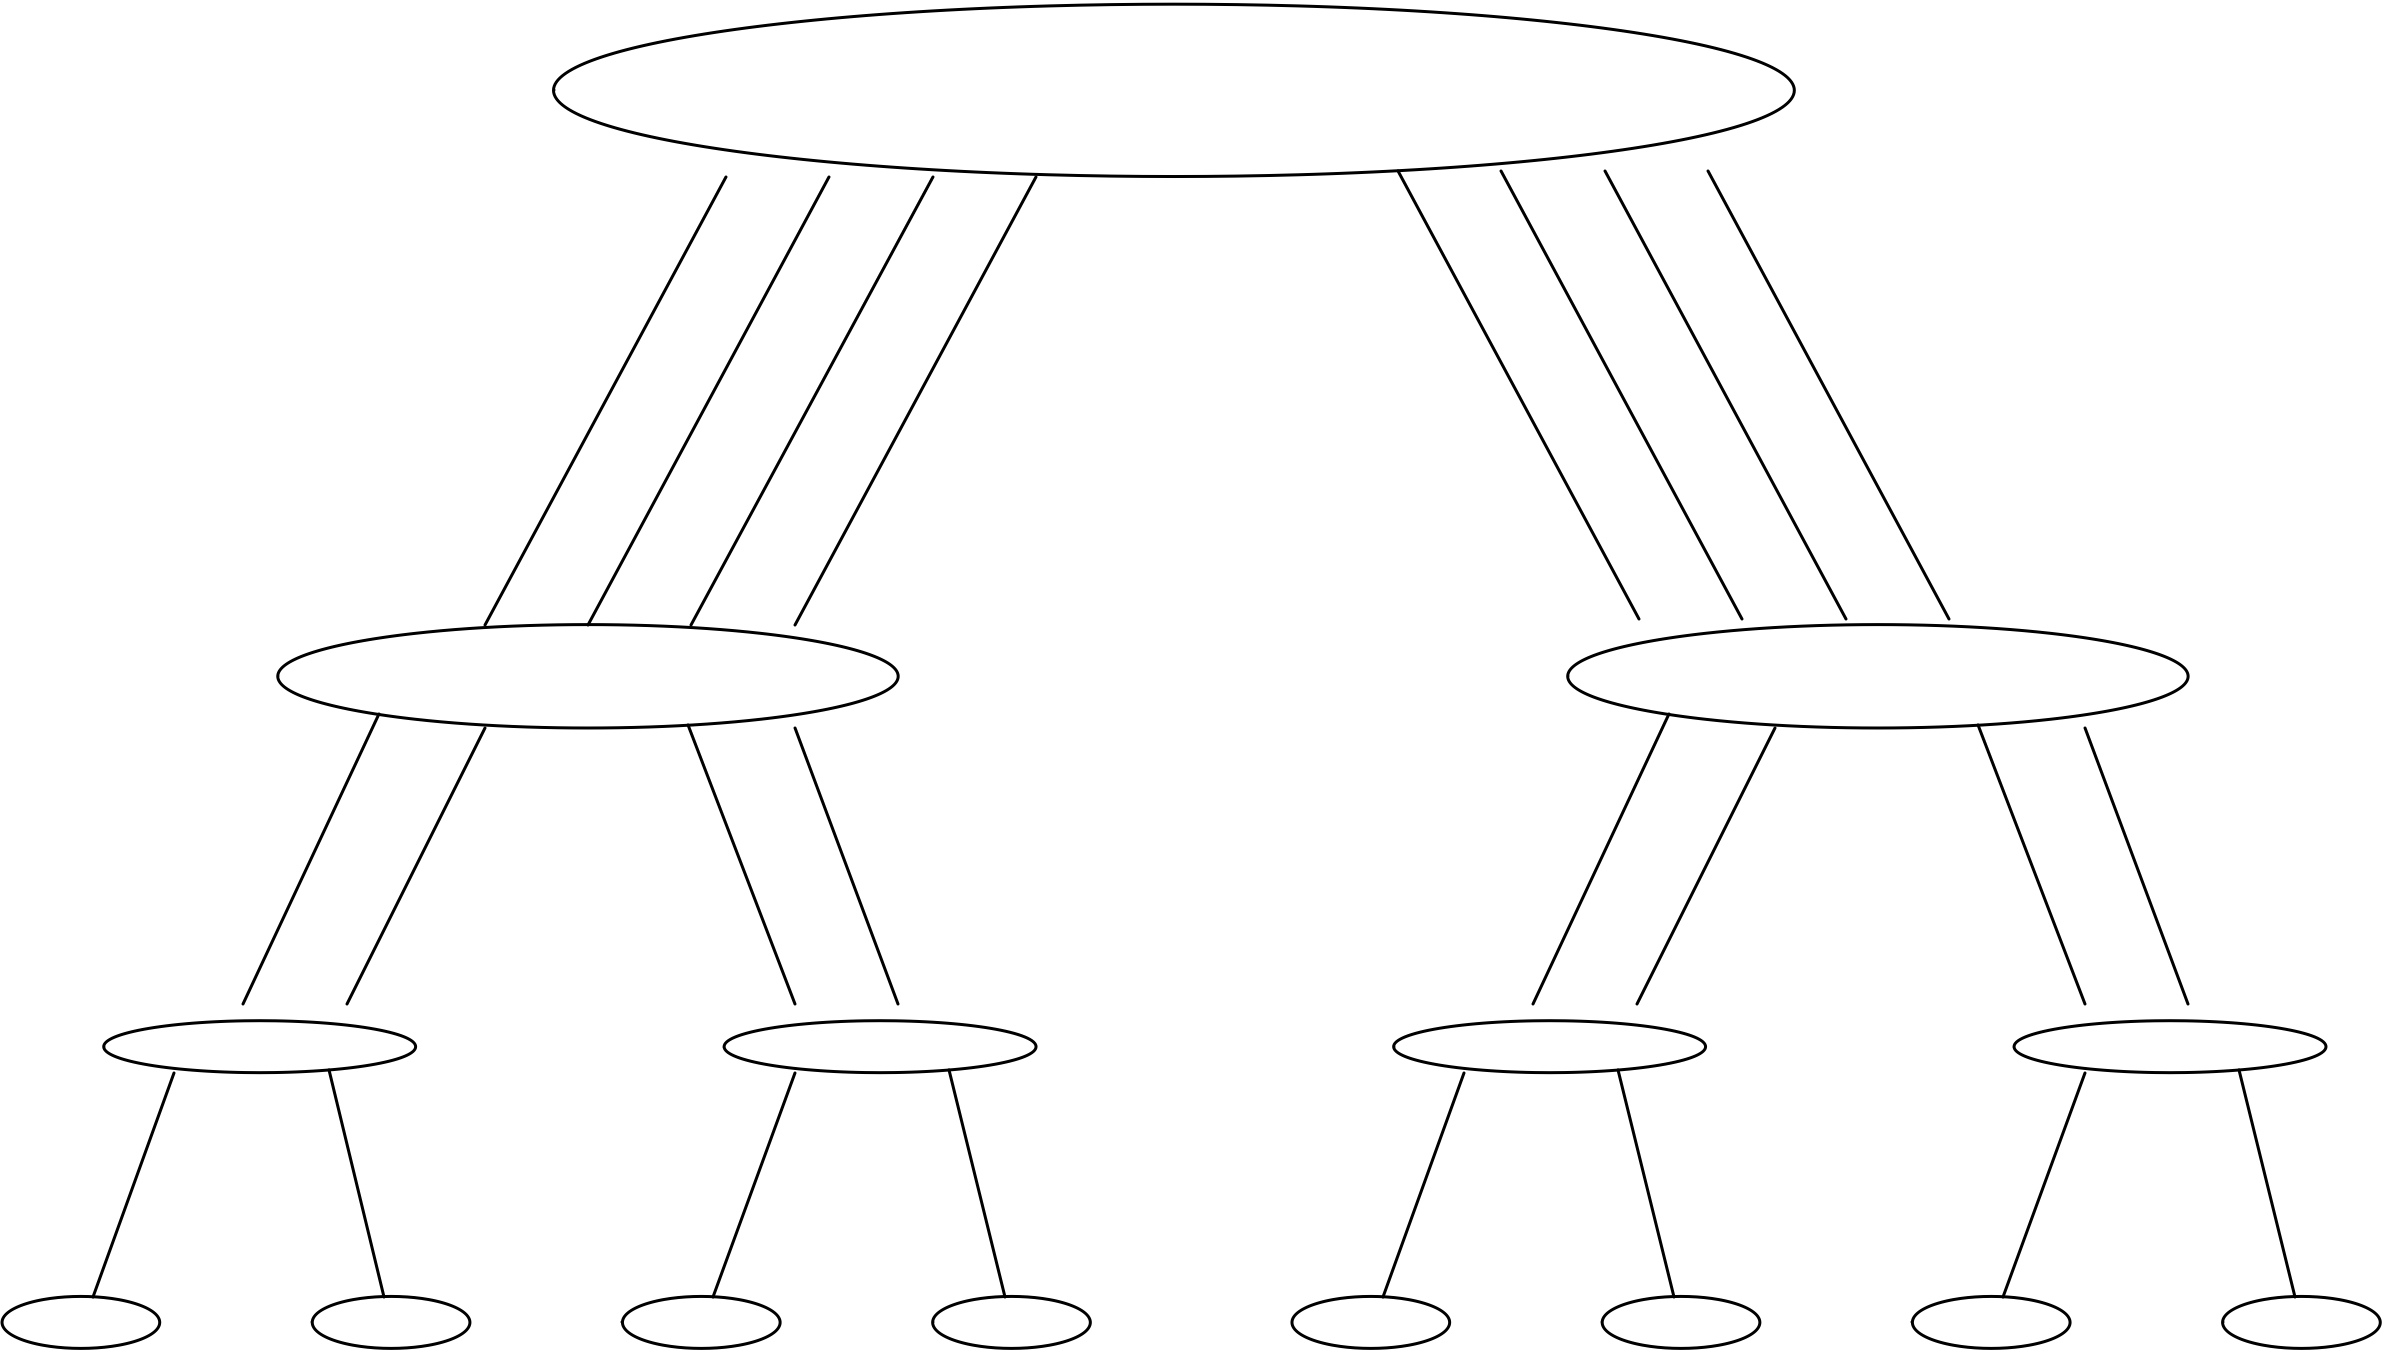
\includegraphics[scale=.1]{fattree5}
  \kern20pt
  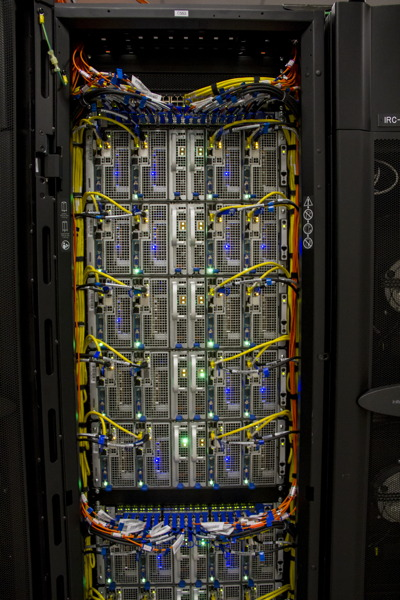
\includegraphics[scale=.8]{stampede_leaf}
}
\end{numberedframe}

\begin{numberedframe}{Fat trees from switching elements}
    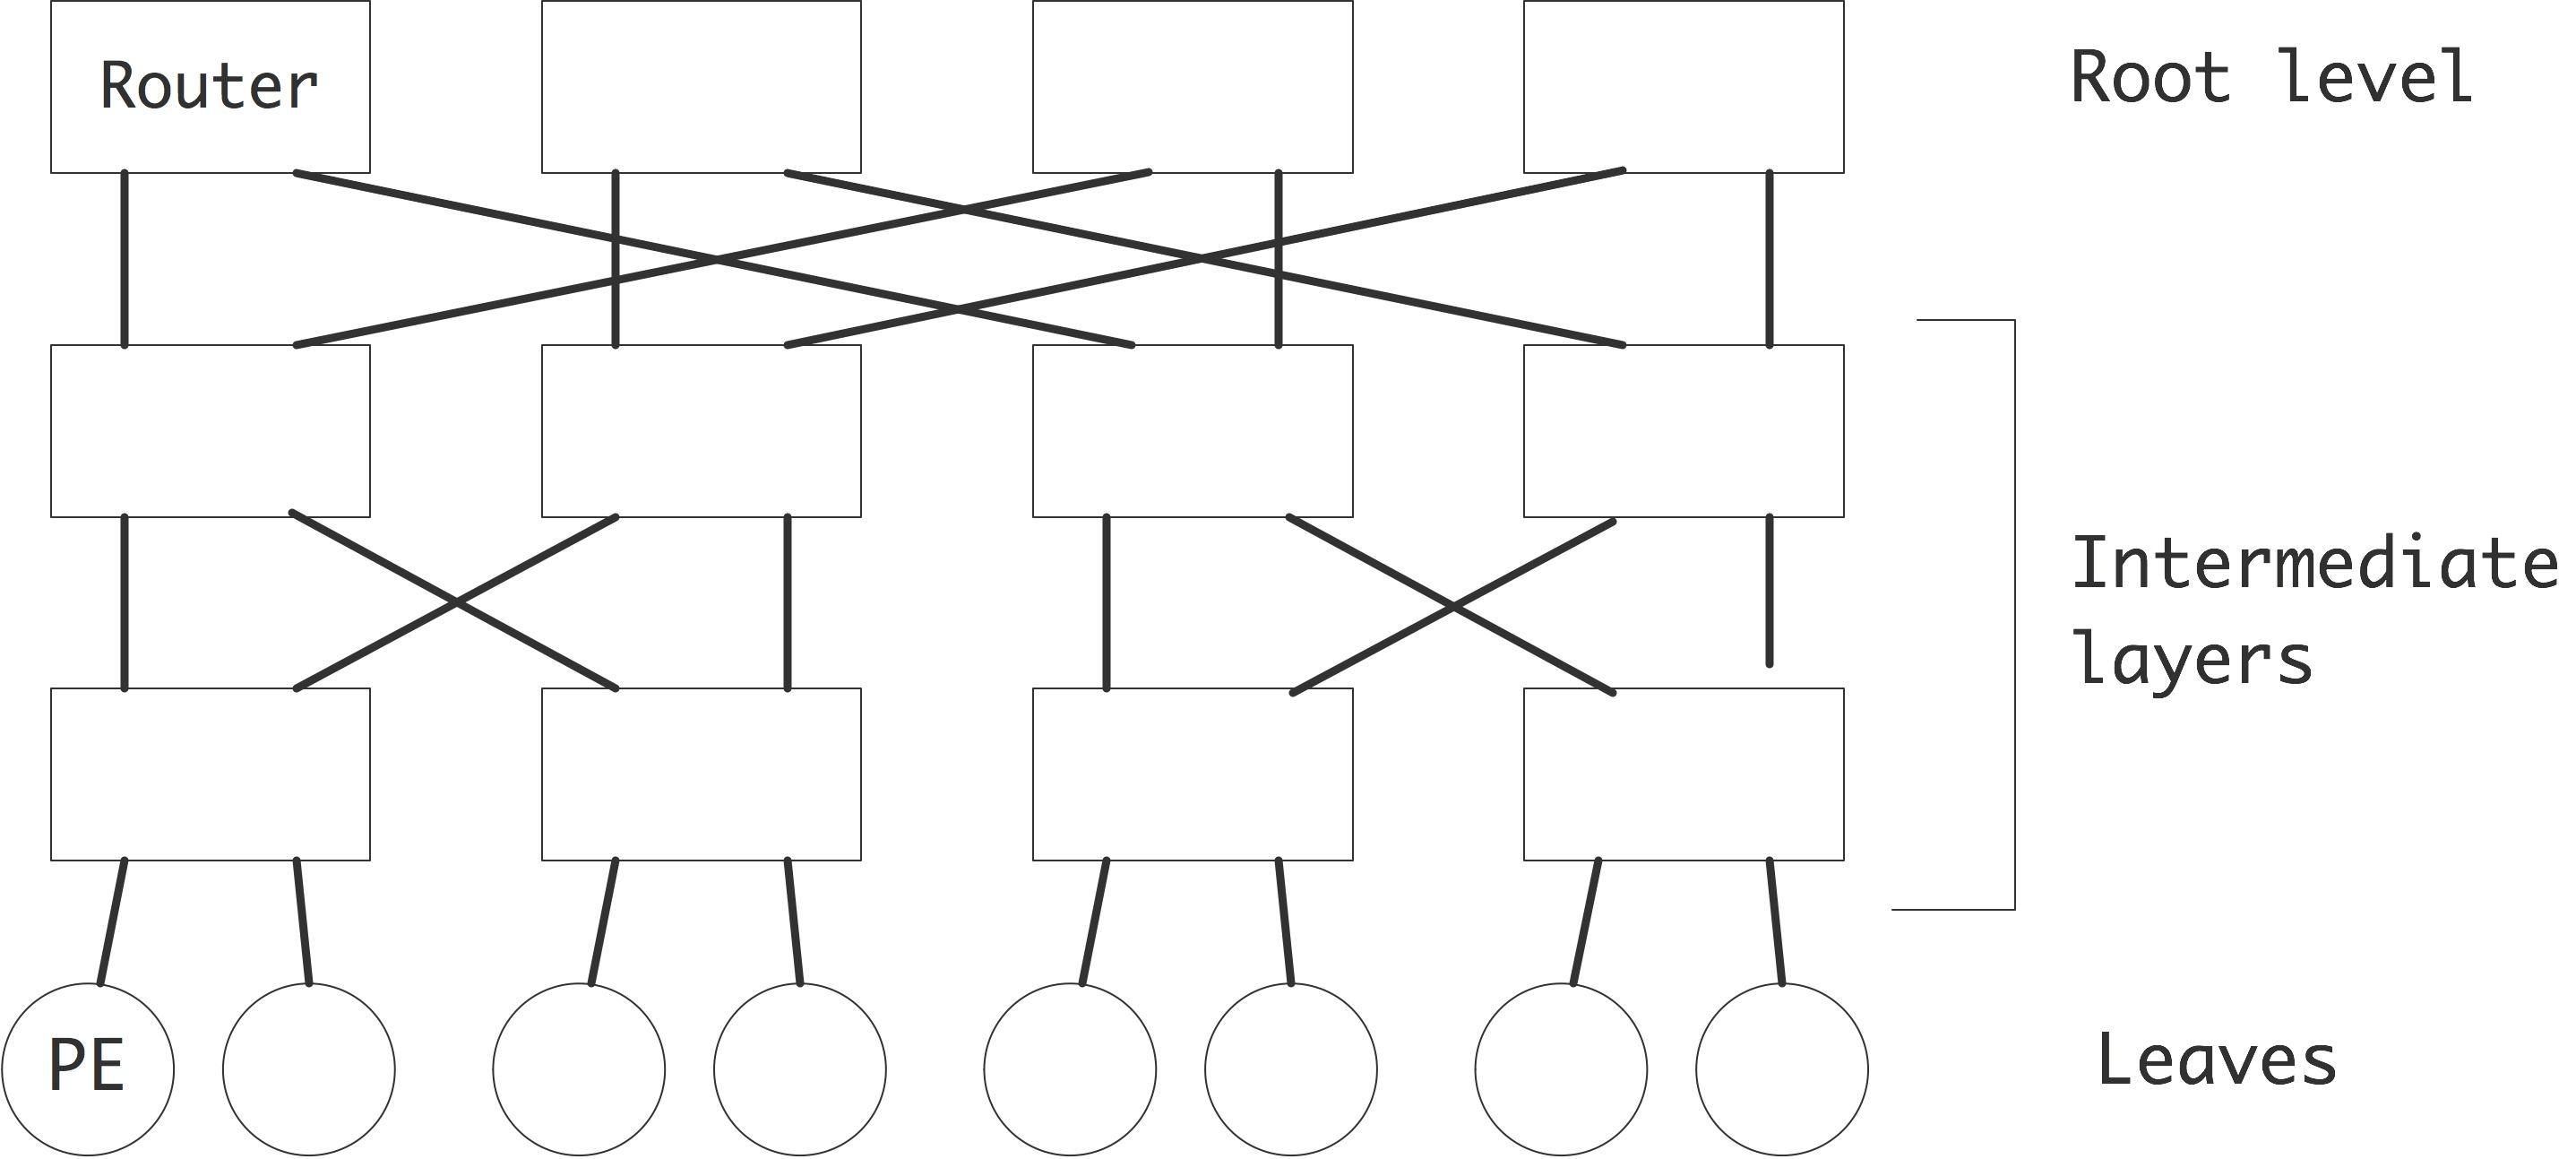
\includegraphics[scale=.11]{fattree-clos}

(Clos network)
\end{numberedframe}

\begin{numberedframe}{Fat tree clusters}
  \hbox{%
    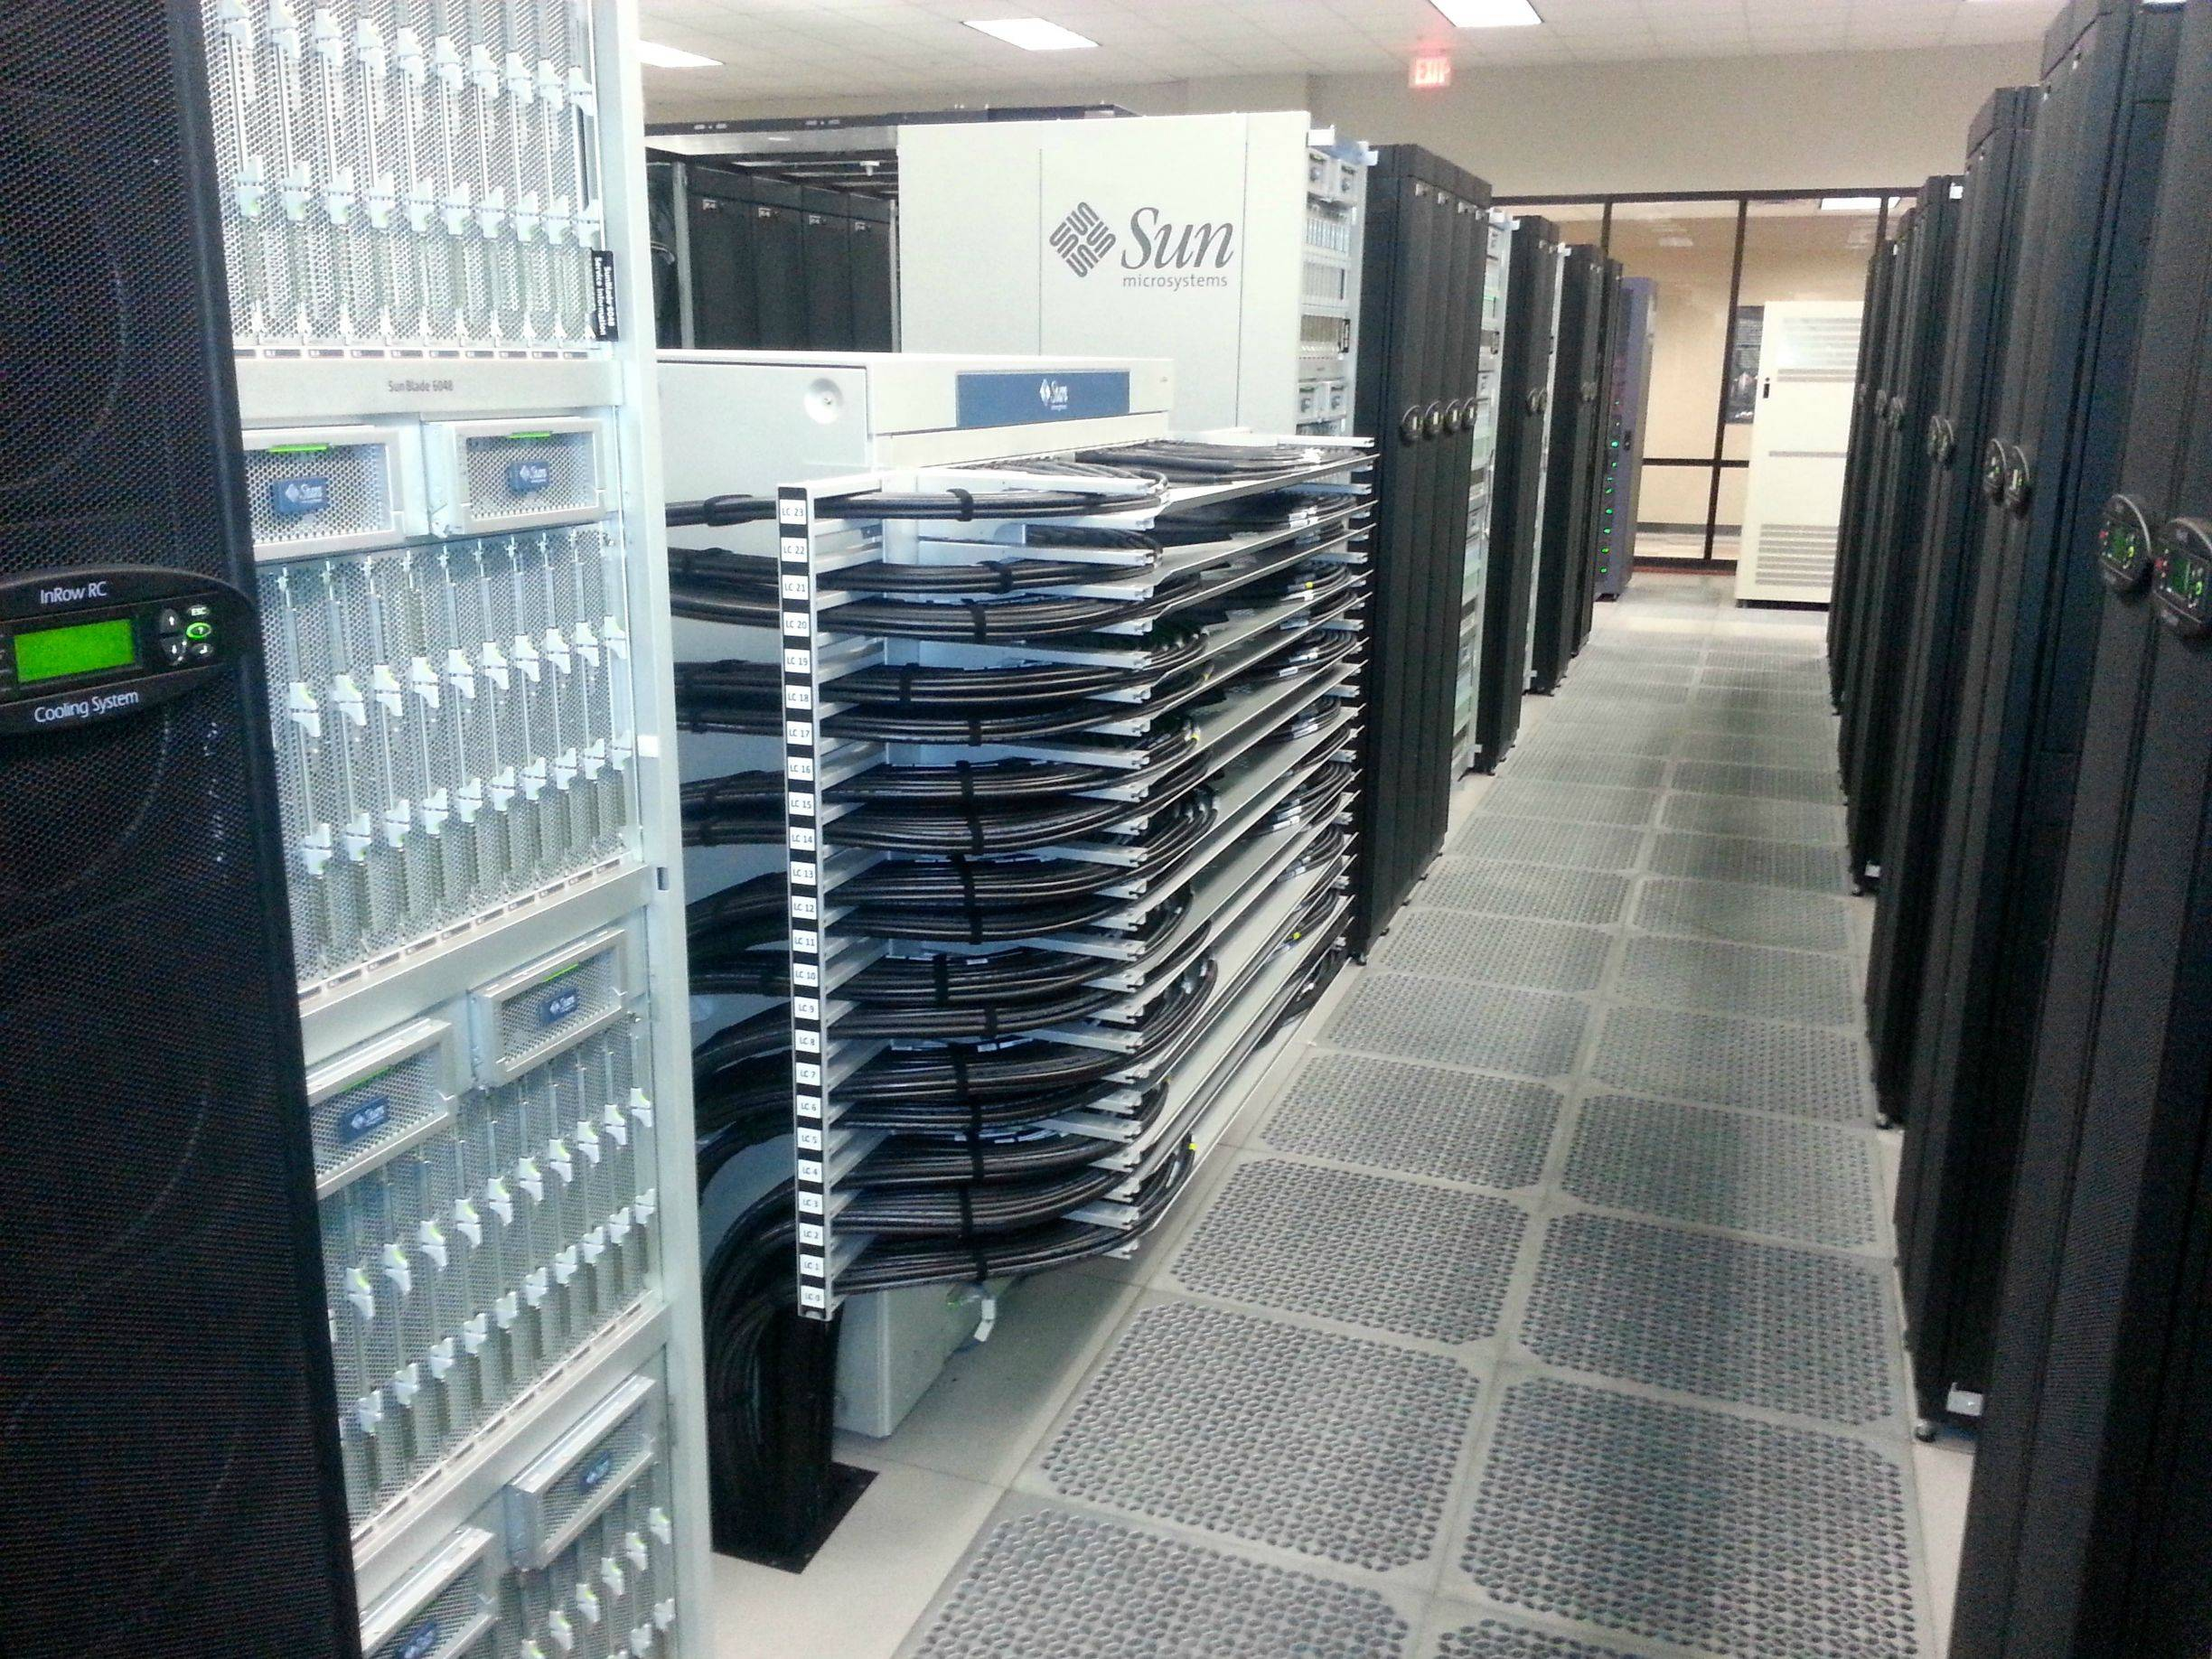
\includegraphics[scale=.06]{rangerswitch}\kern1cm
    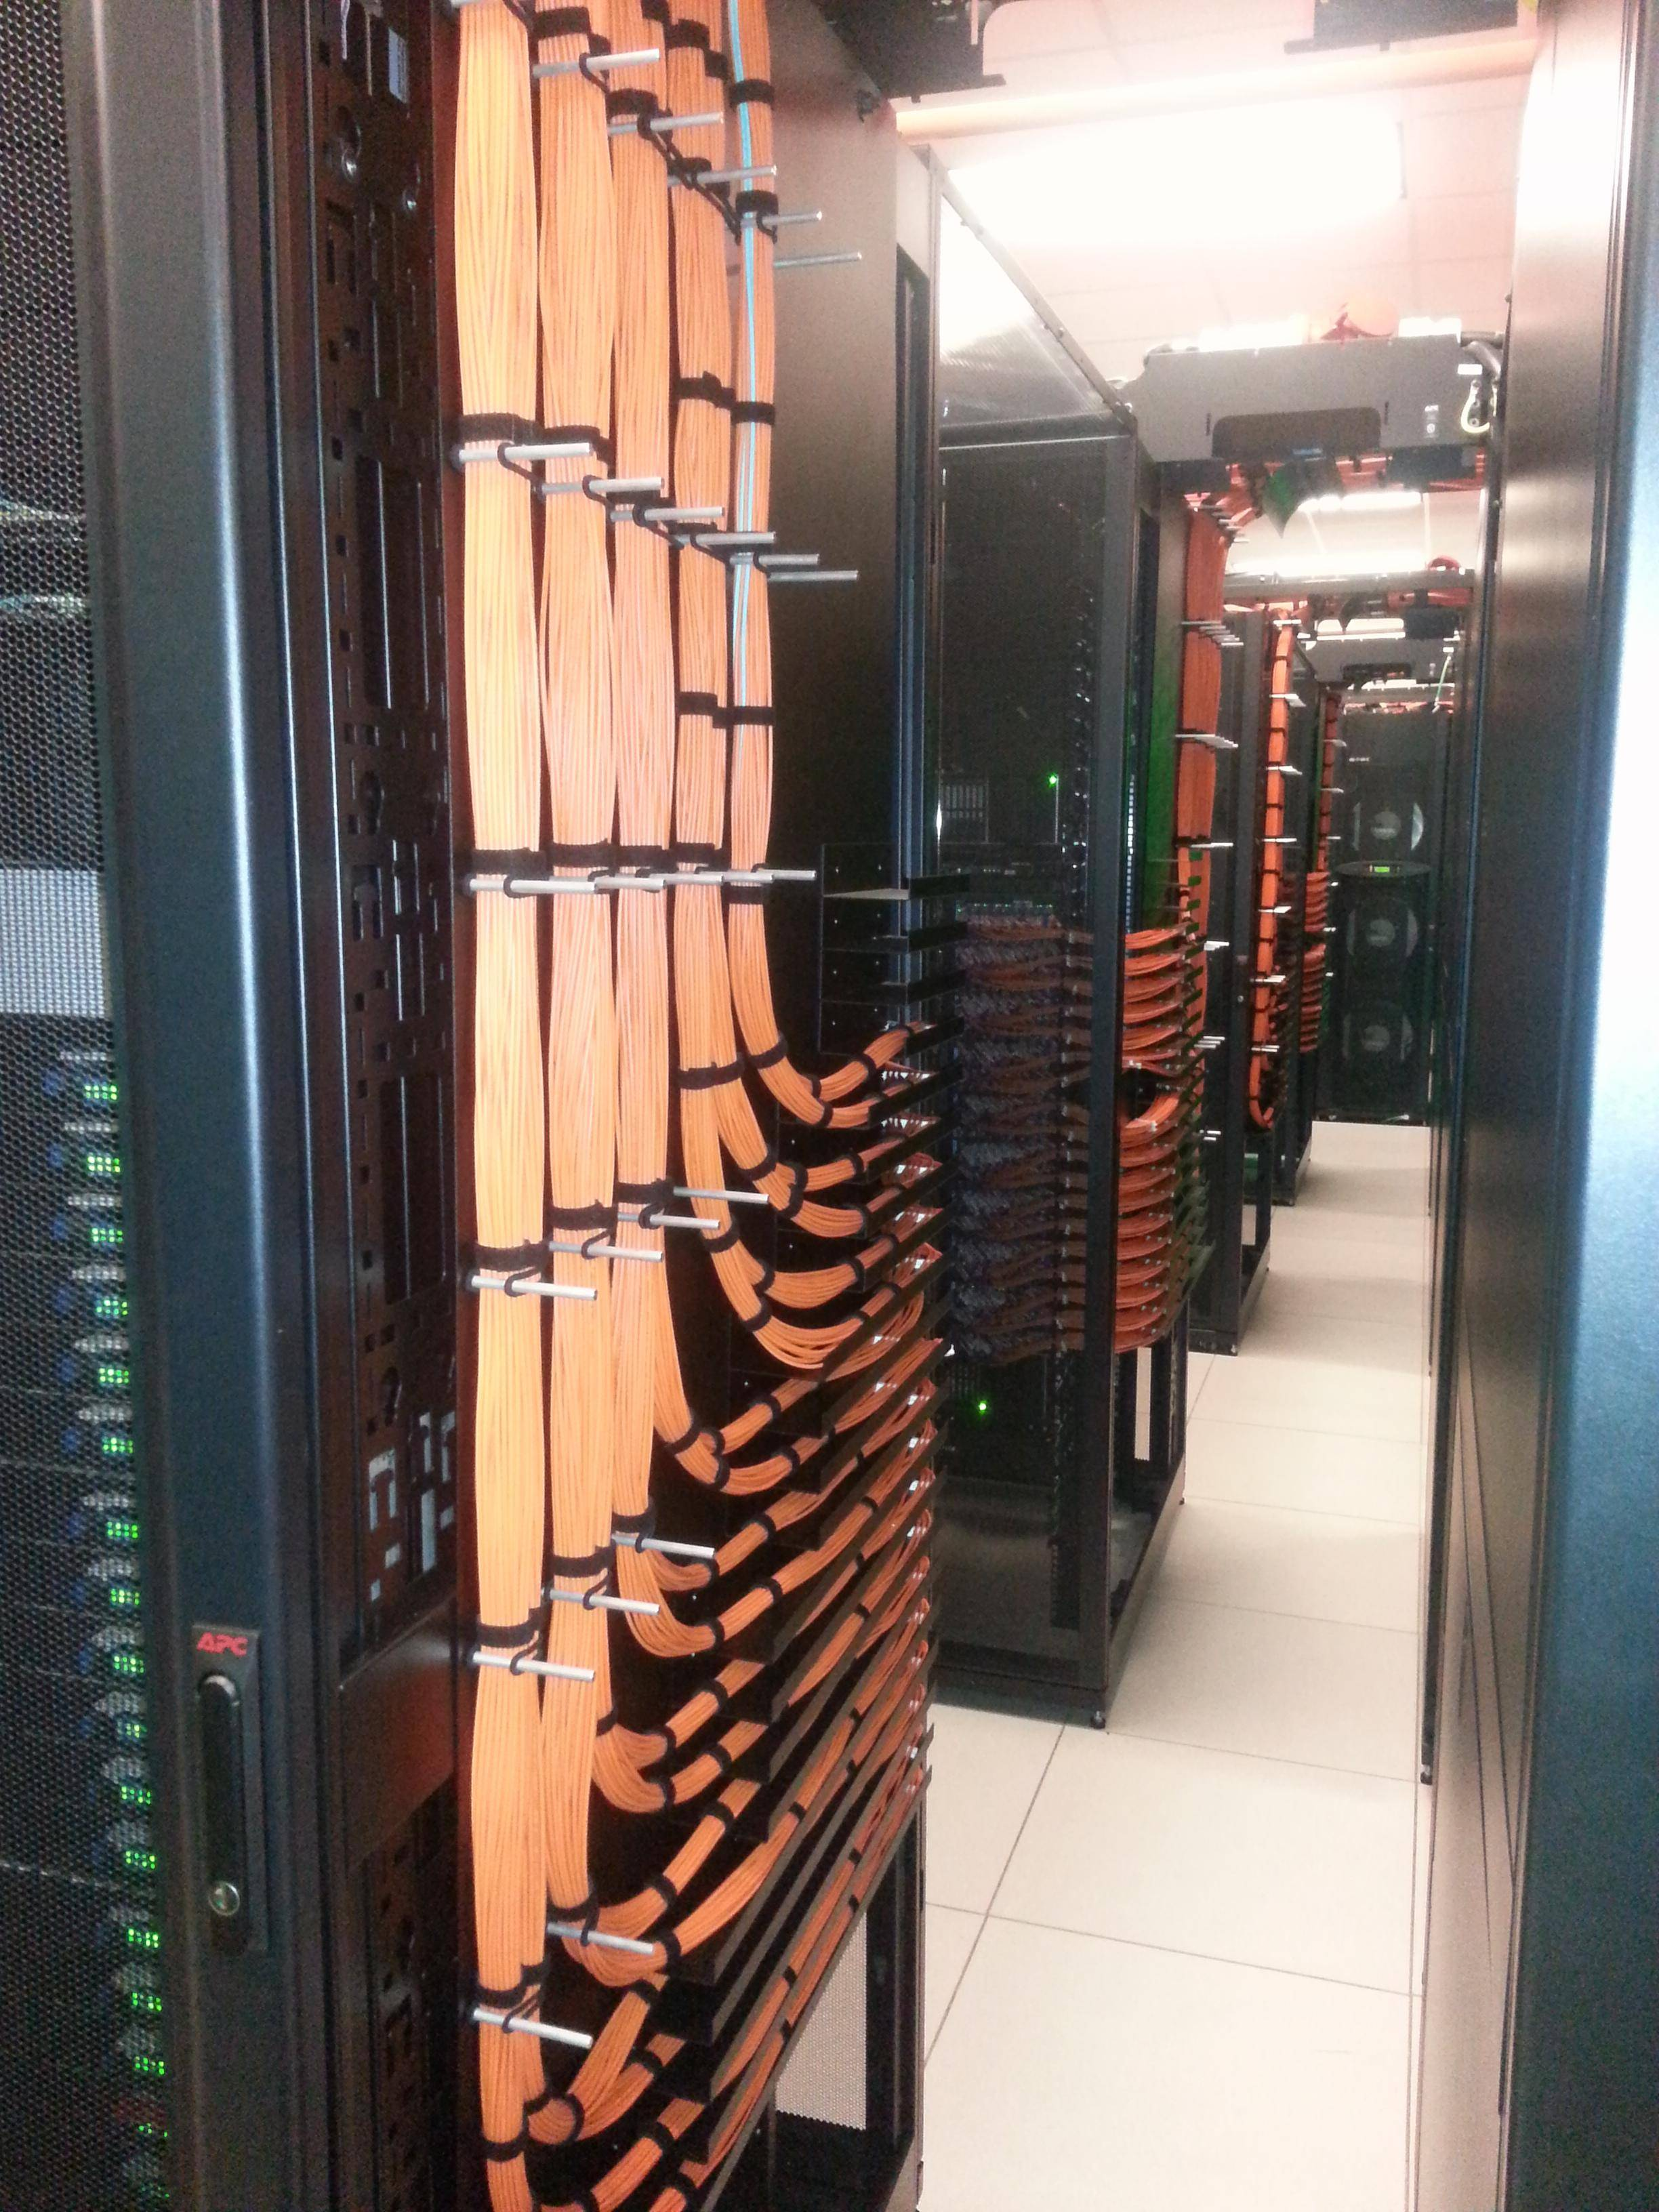
\includegraphics[scale=.05]{stampedeswitches}%
  }
\end{numberedframe}

\begin{exercise}{Switch contention}
  Suppose the number of processor~$p$ is larger than the number of wires~$w$.\\
  Write a simulation that investigates the probability of contention if you
  send $m\leq w$ message to distinct processors.\\
  Can you do a statistical analysis, starting with a simple case?

  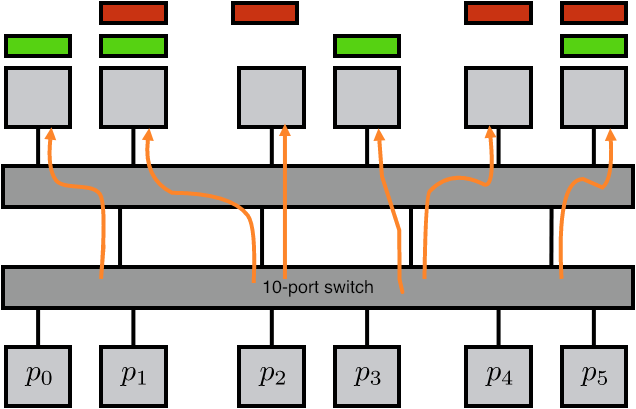
\includegraphics[scale=.3]{switchcontention}
\end{exercise}

\begin{numberedframe}{Mesh clusters}
  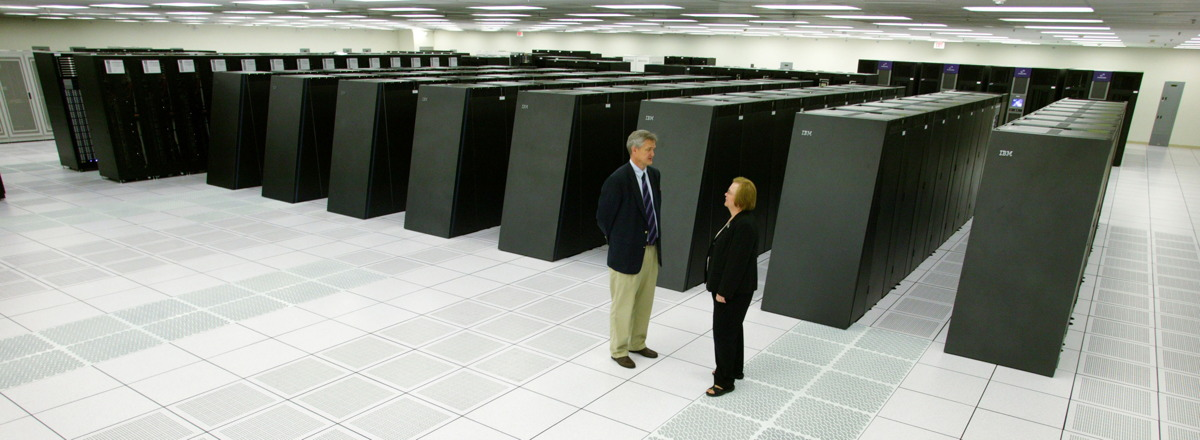
\includegraphics[scale=.45]{bluegenellnl}
\end{numberedframe}
 
\begin{numberedframe}{Levels of locality}
  \begin{itemize}
  \item Core level: private cache, shared cache
  \item Node level: numa
  \item Network: levels in the switch
  \end{itemize}
\end{numberedframe}

\Level 1 {Programming models}

\begin{numberedframe}{Shared vs distributed memory programming}
  Different memory models:

    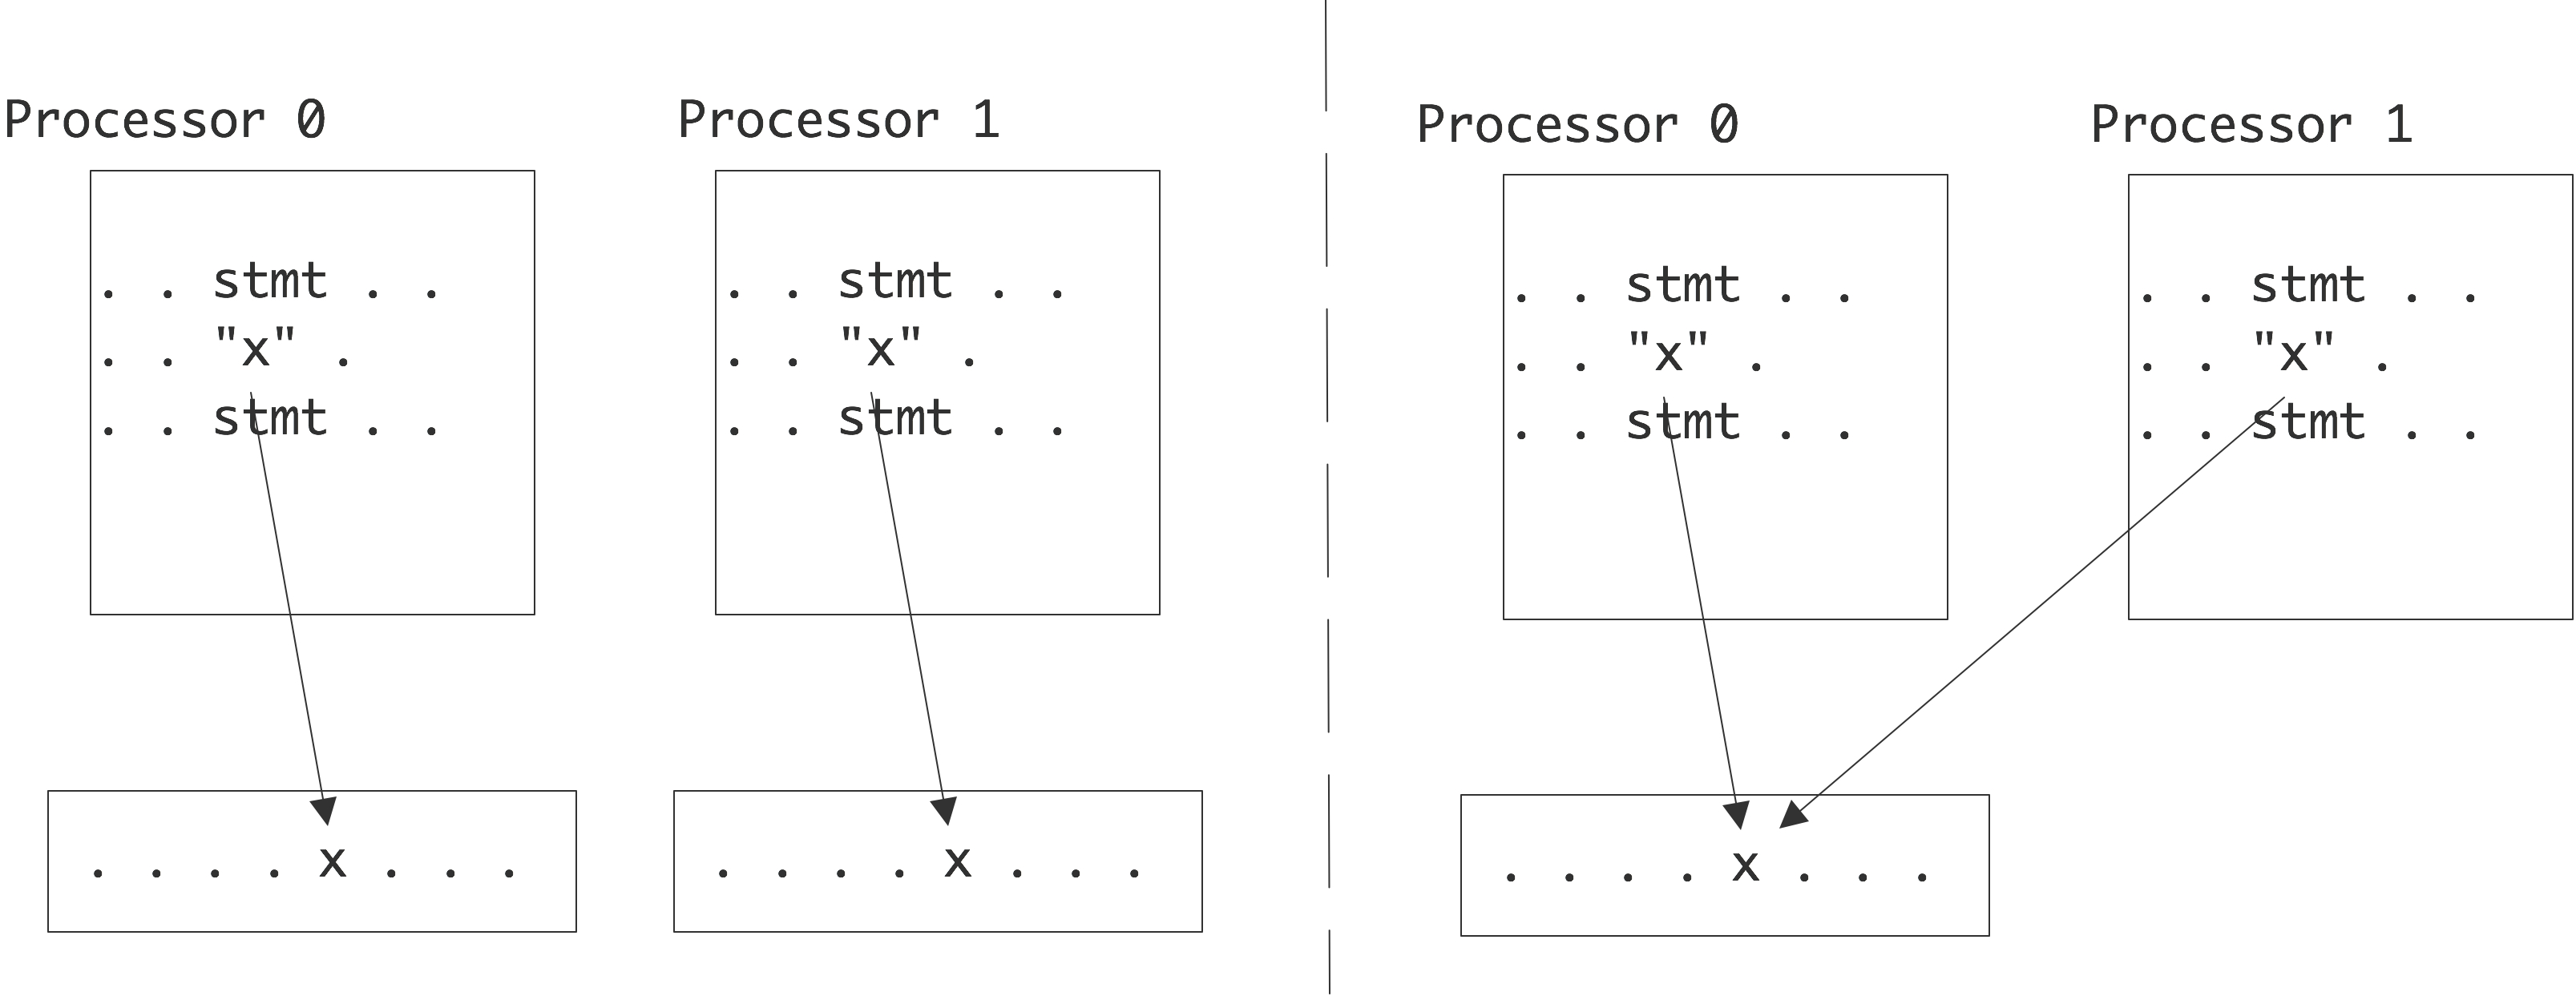
\includegraphics[scale=.08]{shared-distributed}

    Different questions:
    \begin{itemize}
    \item Shared memory: synchronization problems such as critical sections
    \item Distributed memory: data motion
    \end{itemize}
\end{numberedframe}

\Level 2 {Thread parallelism}

\begin{numberedframe}{What is a thread}
  \begin{itemize}
  \item Process: code, heap, stack
  \item Thread: same code but private program counter, stack, local variables
  \item dynamically (even recursively) created: fork-join
  \end{itemize}
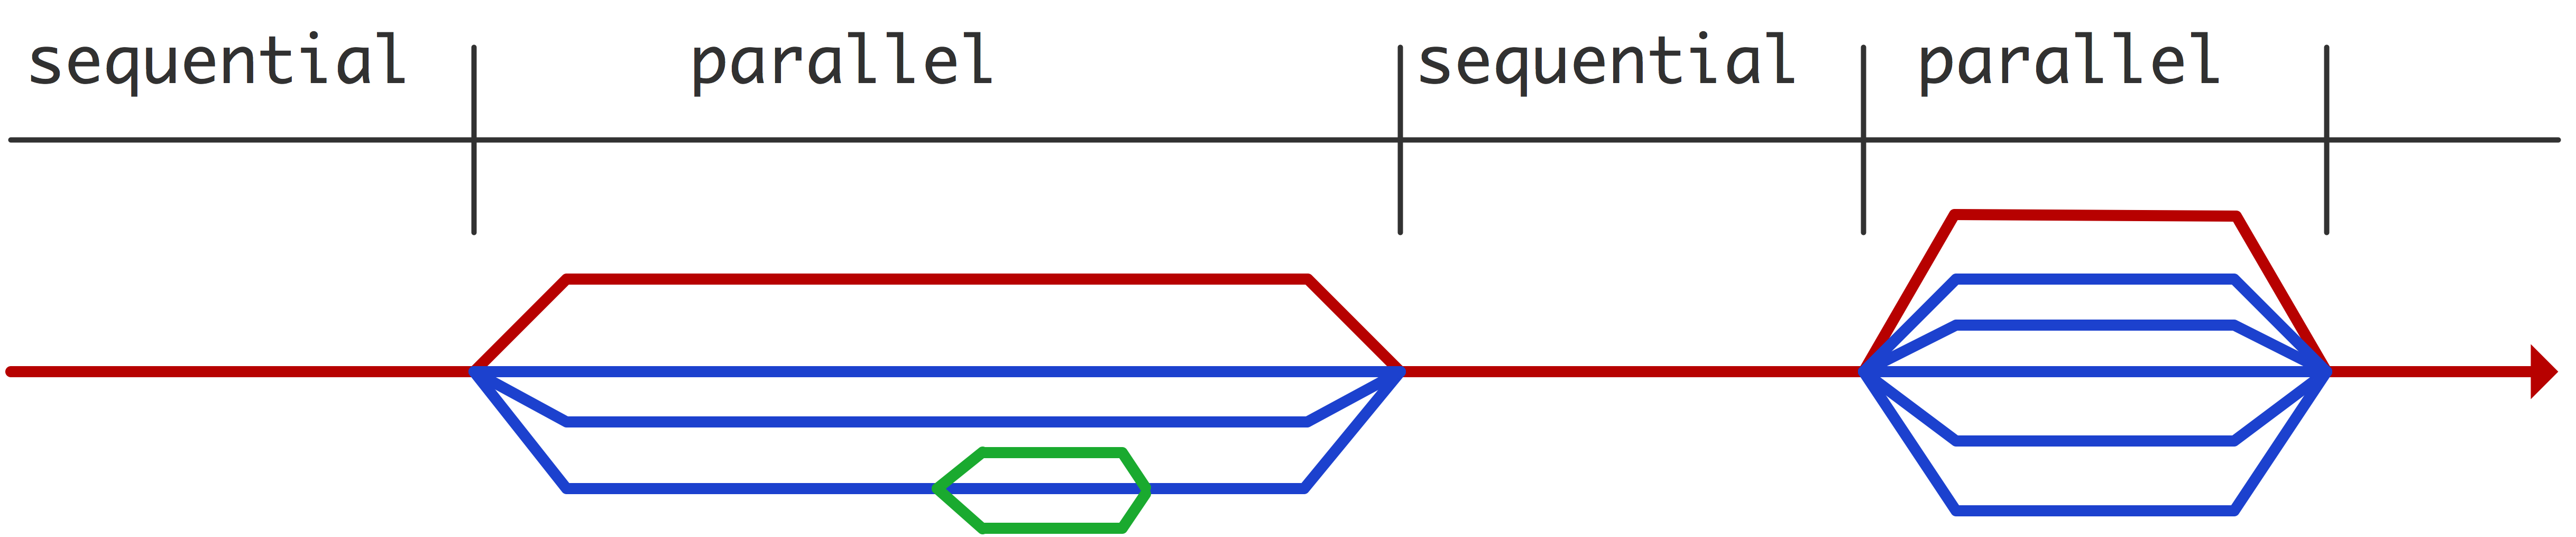
\includegraphics[scale=.06]{fork-join}

Incremental parallelization!
\end{numberedframe}

\begin{numberedframe}{Thread context}
  \begin{itemize}
  \item Private data (stack, local variables) is called `thread context'
  \item Context switch: switch from one thread execution to another
  \item context switches are expensive; alternative hyperthreading
  \item Intel Xeon Phi: hardware support for 4 threads per core
  \item GPUs: fast context switching between many threads
  \end{itemize}
\end{numberedframe}

\begin{numberedframe}{Thread programming 1}
Pthreads
\begin{lstlisting}
pthread_t threads[NTHREADS];
printf("forking\n");
for (i=0; i<NTHREADS; i++)
    if (pthread_create(threads+i,NULL,&adder,NULL)!=0)
        return i+1;
printf("joining\n");
for (i=0; i<NTHREADS; i++)
    if (pthread_join(threads[i],NULL)!=0) 
        return NTHREADS+i+1;
\end{lstlisting}
\end{numberedframe}

\begin{numberedframe}{Atomic operations}
\begin{tabbing}
  process 1: \texttt{I=I+2}\\
  process 2: \texttt{I=I+3}
\end{tabbing}
\footnotesize
\begin{tabular}{rrrrrr}
  \toprule
  \multicolumn{2}{c}{scenario 1.}& \multicolumn{2}{|c|}{scenario 2.}&
  \multicolumn{2}{c}{scenario 3.}\\ \midrule
  \multicolumn{6}{c}{$\n{I}=0$}\\ \midrule
  read $\n{I}=0$&read $\n{I}=0$&
    read $\n{I}=0$&read $\n{I}=0$&
      read $\n{I}=0$& \\
  do $\n{I}=2$&do $\n{I}=3$& 
    do $\n{I}=2$&do $\n{I}=3$&
      do $\n{I}=2$& \\
  write $\n{I}=2$& & &write $\n{I}=3$&write $\n{I}=2$& \\
  &write $\n{I}=3$&write $\n{I}=2$& & &read $\n{I}=2$\\
  &&&&&do $\n{I}=5$\\
  &&&&&write $\n{I}=5$\\
  \midrule
  \multicolumn{2}{c}{$\n{I}=3$}& \multicolumn{2}{c}{$\n{I}=2$}&
  \multicolumn{2}{c}{$\n{I}=5$}\\ 
  \bottomrule
\end{tabular}
\end{numberedframe}

\begin{numberedframe}{Dealing with atomic operations}
  Semaphores, locks, mutexes, critical sections, transactional memory

  Software / hardware
\end{numberedframe}

\begin{numberedframe}{Cilk}
\index{Cilk}
\small
\hbox{%
  \kern 10pt
  \begin{minipage}{2in}\tt
    \begin{tabbing}
      \textit{Sequential code:}\\  
      int \=fib(int n)\{ \\
      \>if (n<2) return 1;\\
      \>else \=\{\\
      \>\>int rst=0;\\
      \>\>rst += fib(n-1);\\
      \>\>rst += fib(n-2);\\
      \>\>return rst;\\
      \}\\
    \end{tabbing}
      \end{minipage}
  \kern 10pt
  \begin{minipage}{2in}\tt
    \begin{tabbing}
      \textit{Cilk code:}\\  
      cilk \=int fib(int n)\{ \\
      \>if (n<2) return 1;\\
      \>else \=\{\\
      \>\>int rst=0;\\
      \>\>rst += spawn fib(n-1);\\
      \>\>rst += spawn fib(n-2);\\
      \>\>sync;\\
      \>\>return rst;\\
      \}\\
    \end{tabbing}
      \end{minipage}
}

Sequential consistency: program output identical to sequential
\end{numberedframe}

\begin{numberedframe}{OpenMP}
  \begin{itemize}
  \item Directive based
  \item Parallel sections, parallel loops, tasks
  \end{itemize}
\end{numberedframe}

\Level 2 {Distributed memory parallelism}

\begin{numberedframe}{Global vs local view}
  \[ 
\begin{cases}
y_i\leftarrow y_i+x_{i-1}&i>0\\ \mbox{$y_i$ unchanged}&i=0
\end{cases}
\]
\begin{itemize}
\item If I am processor~0 do nothing, otherwise receive a $y$ element
  from the left, add it to my $x$ element.
\item If I am the last processor do nothing, otherwise send my $y$
  element to the right.
\end{itemize}
(Let's think this through\ldots)
\end{numberedframe}

\begin{numberedframe}{Global picture}
  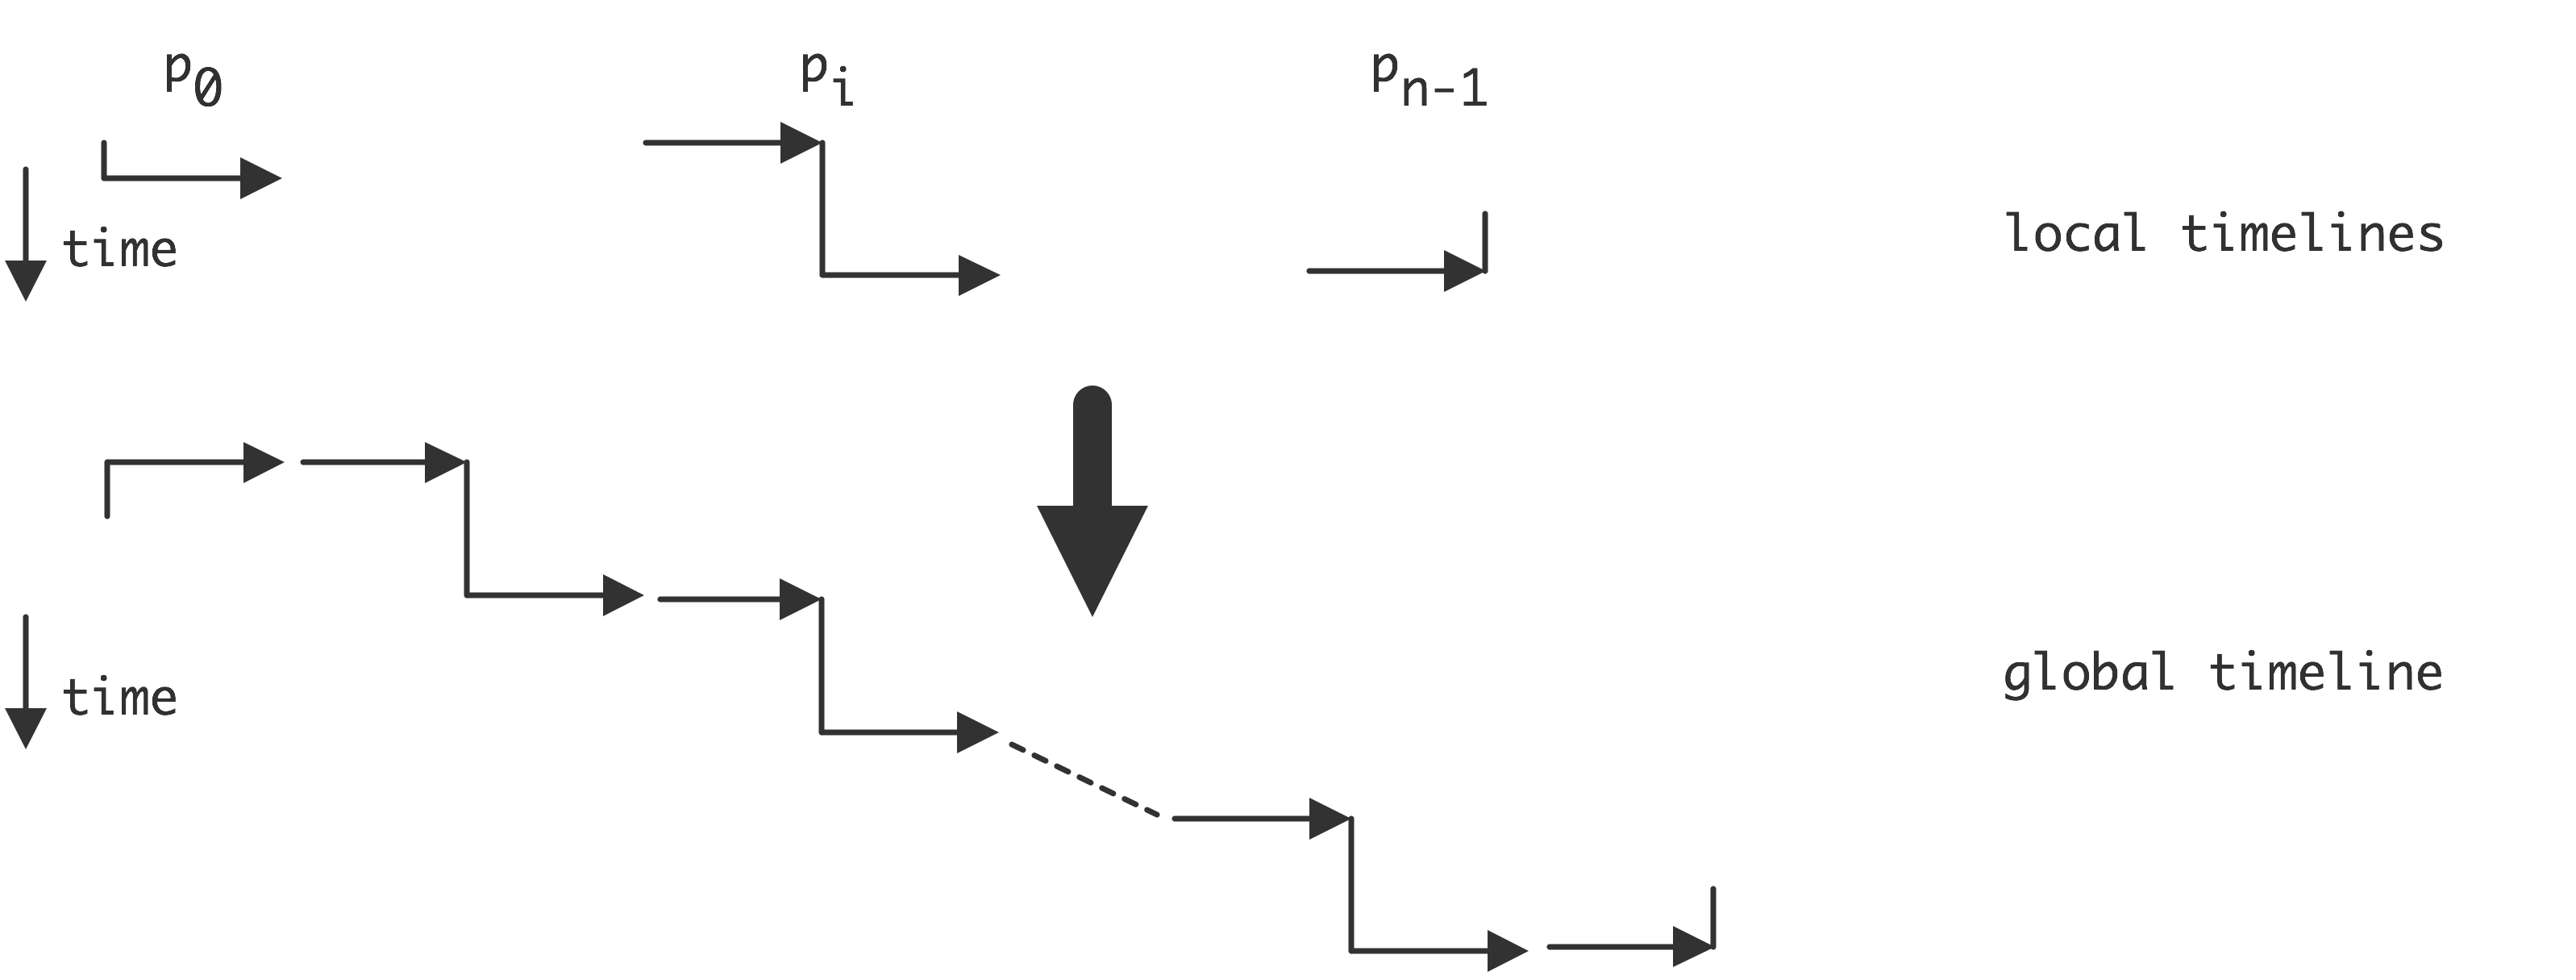
\includegraphics[scale=.1]{wave_right_1}  
\end{numberedframe}

\begin{numberedframe}{Careful coding}
  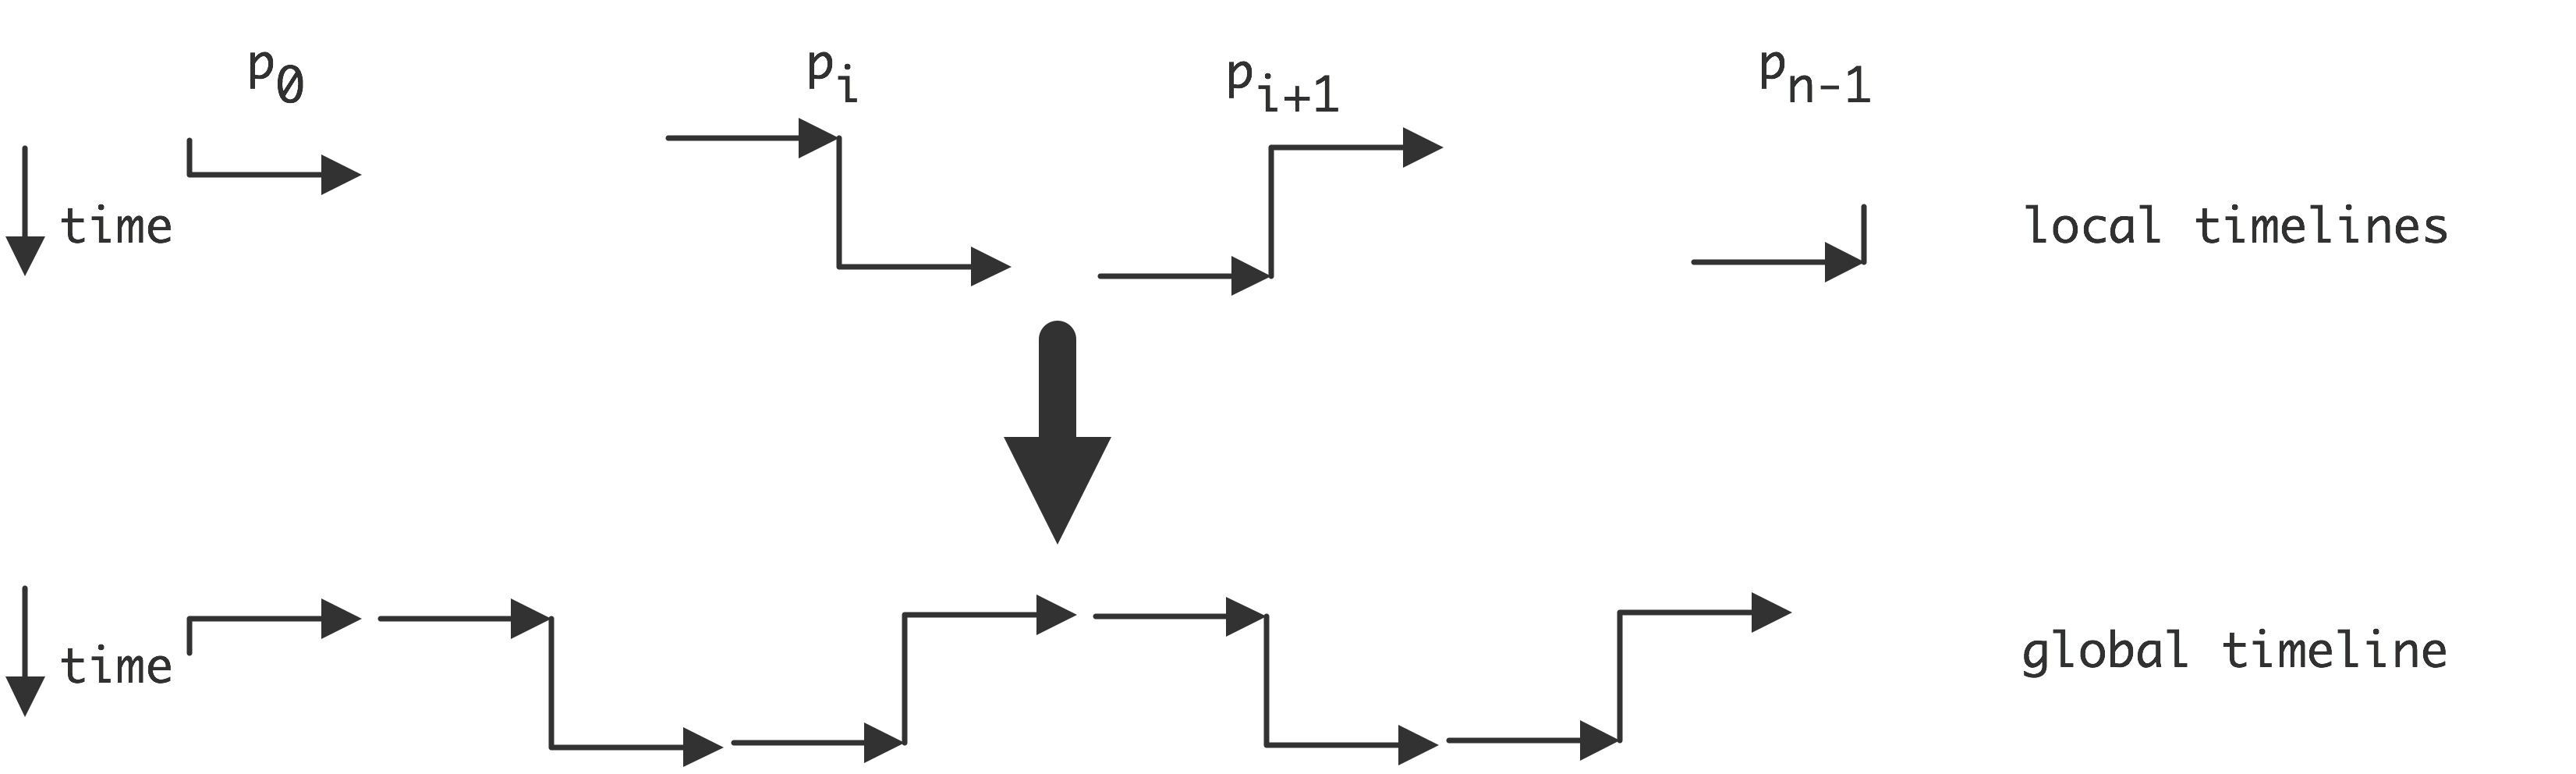
\includegraphics[scale=.1]{wave_right_3}  
\end{numberedframe}

\begin{numberedframe}{Better approaches}
  \begin{itemize}
  \item Non-blocking send/receive
  \item One-sided
  \end{itemize}
\end{numberedframe}

\Level 2 {Hybrid/heterogeneous parallelism}

\begin{numberedframe}{Hybrid computing}
  \begin{itemize}
  \item Use MPI between nodes, OpenMP inside nodes
  \item alternative: ignore shared memory and MPI throughout
  \item you save: buffers and copying
  \item bundling communication, load spread 
  \end{itemize}
\end{numberedframe}

\begin{numberedframe}{Using threads for load balancing}
  Dynamic scheduling gives load balancing

  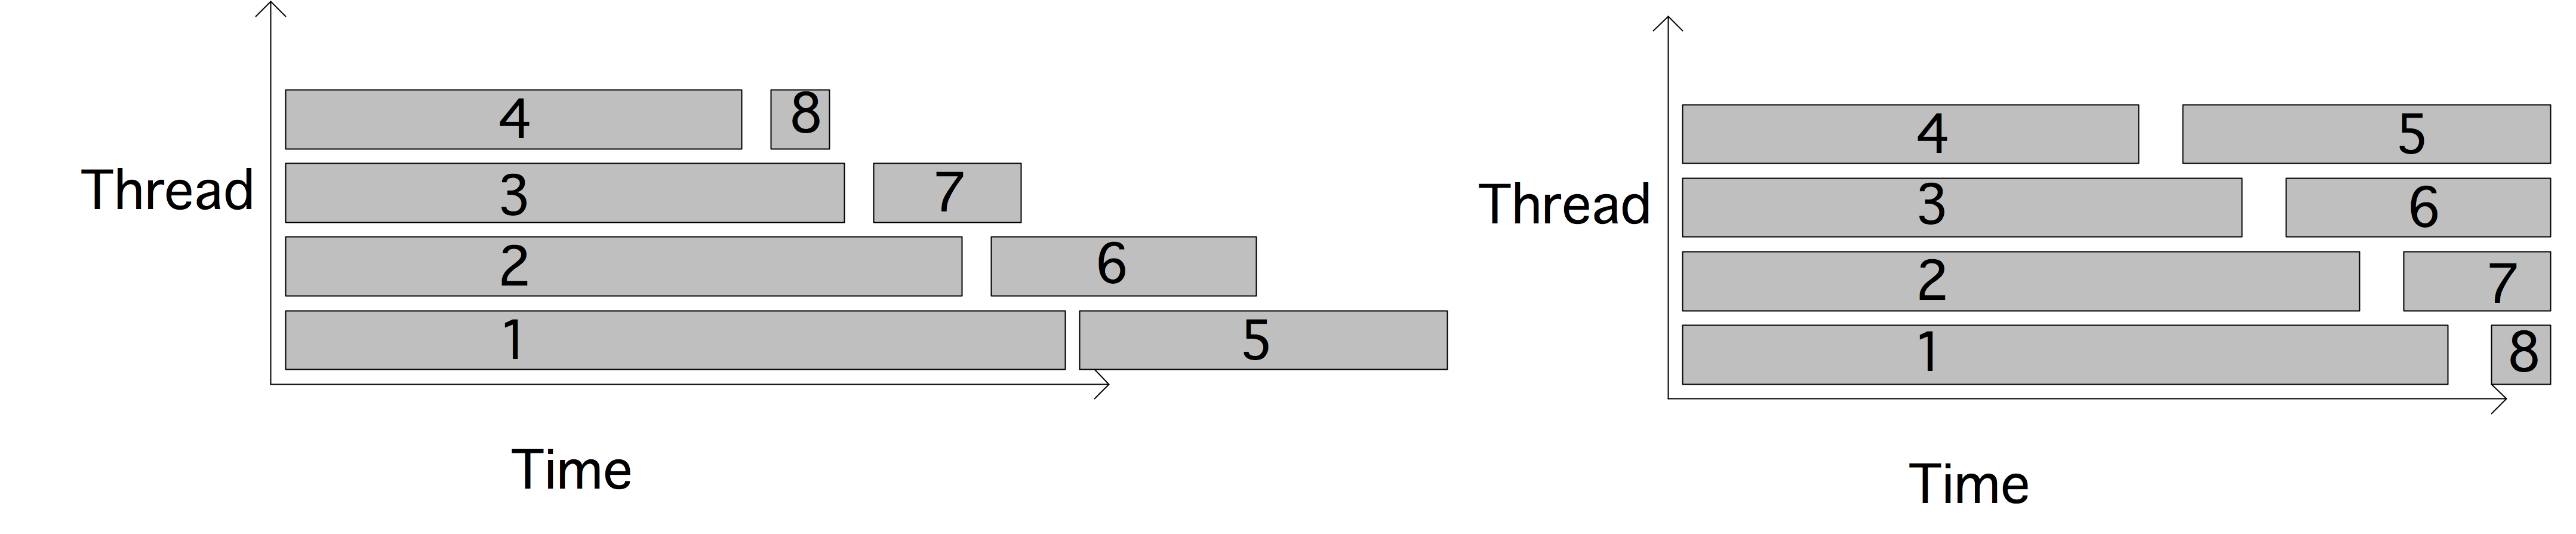
\includegraphics[scale=.1]{scheduling}

  Hybrid is possible improvement over strict-MPI
\end{numberedframe}

\begin{numberedframe}{Amdahl's law for hybrid programming}
  \begin{itemize}
  \item $p$ nodes with $c$ cores each
  \item $F_p$ core-parallel fraction, assume full MPI parallel
  \item ideal speedup $p c$, running time $T_1/(pc)$, actually:
    \[
    T_{p,c} = T_1 \left(\frac {F_s}{p} + \frac{F_p}{p c}\right)
    = \frac{T_1}{pc}\left( F_sc+F_p\right) 
    = \frac{T_1}{pc}\left( 1+ F_s(c-1)\right).
    \]
    \item $T_1/T_{p,c} \approx p/F_s$
    \item Original Amdahl: $S_p<1/F_s$, hybrid programming $S_p<p/F_s$
  \end{itemize}
\end{numberedframe}

\Level 2 {Design patterns}

\begin{numberedframe}{Array of Structures}
\begin{lstlisting}
struct { int number; double xcoord,ycoord; } _Node;
struct { double xtrans,ytrans} _Vector;
typedef struct _Node* Node;
typedef struct _Vector* Vector;
\end{lstlisting}
\begin{lstlisting}
Node *nodes = (node) malloc( n_nodes*sizeof(struct _Node) );
\end{lstlisting}
\end{numberedframe}

\begin{numberedframe}{Operations}
Operate
\begin{lstlisting}
void shift(node the_point,vector by) {
  the_point->xcoord += by->xtrans;
  the_point->ycoord += by->ytrans;
}
\end{lstlisting}
in a loop
\begin{lstlisting}
for (i=0; i<n_nodes; i++) {
  shift(nodes[i],shift_vector);
}
\end{lstlisting}
\end{numberedframe}

\begin{numberedframe}{Along come the 80s}
Vector operations
\begin{lstlisting}
node_numbers = (int*) malloc( n_nodes*sizeof(int) );
node_xcoords = // et cetera
node_ycoords = // et cetera
\end{lstlisting}
and you would iterate
\begin{lstlisting}
for (i=0; i<n_nodes; i++) {
  node_xoords[i] += shift_vector->xtrans;
  node_yoords[i] += shift_vector->ytrans;
}
\end{lstlisting}
\end{numberedframe}

\begin{numberedframe}{and the wheel of reinvention turns further}
  The original design was better for MPI in the 1990s

  except when vector instructions (and GPUs) came along in the 2000s
\end{numberedframe}

\begin{numberedframe}{Latency hiding}
  \begin{itemize}
  \item Memory and network are slow, prevent having to wait for it
  \item Hardware magic: out-of-order execution, caches, prefetching
  \end{itemize}
\end{numberedframe}

\begin{numberedframe}{Explicit latency hiding}
Matrix vector product
\[ \forall_{i\in I_p}\colon y_i=\sum_j a_{ij}x_j. \]
$x$ needs to be gathered:
\[ \forall_{i\in I_p}\colon y_i=
  \left(\sum_{\mbox{\small $j$ local}}
    +\sum_{\mbox{\small $j$ not local}} \right) a_{ij}x_j. 
\]
Overlap loads and local operations

Possible in MPI and Xeon Phi offloading,\\
very hard to do with caches  
\end{numberedframe}

\Level 2 {What's left}

\begin{numberedframe}{Parallel languages}
  \begin{itemize}
  \item Co-array Fortran: extensions to the Fortran standard
  \item X10
  \item Chapel
  \item UPC
  \item BSP
  \item MapReduce
  \item Pregel,~\ldots
  \end{itemize}
\end{numberedframe}

\begin{numberedframe}{UPC example}
\begin{lstlisting}
#define N 100*THREADS

shared int v1[N], v2[N], v1plusv2[N];

void main()
{
  int i;
  upc_forall(i=0; i<N; i++; i)
    v1plusv2[i]=v1[i]+v2[i];
}
\end{lstlisting}
\end{numberedframe}

\begin{numberedframe}{Co-array Fortran example}
Explicit dimension for `images':
\begin{lstlisting}
Real,dimension(100),codimension[*] :: X
Real :: X(100)[*]
Real :: X(100,200)[10,0:9,*]
\end{lstlisting}
determined by runtime environment
\end{numberedframe}

\begin{numberedframe}{Grab bag of other approaches}
  \begin{itemize}
  \item OS-based: data movement induced by cache misses
  \item Active messages: application level Remote Procedure Call\\
    (see: Charm++)
  \end{itemize}
\end{numberedframe}

\Level 1 {Load balancing, locality, space-filling curves}

\begin{numberedframe}{The load balancing problem}
  \begin{itemize}
  \item Application load can change dynamically\\
    e.g., mesh refinement, time-dependent problems
  \item Splitting off and merging loads 
  \item No real software support: write application anticipating load management
  \item Initial balancing: graph partitioners
  \end{itemize}
\end{numberedframe}

\begin{numberedframe}{Load balancing and performance}
  \begin{itemize}
  \item Assignment to arbitrary processor violates locality
  \item Need a dynamic load assignment scheme that preserves
    locality under load migration
  \item Fairly easy for regular problems, for irregular?
  \end{itemize}
\end{numberedframe}

\Level 2 {Space-filling curves}

\begin{numberedframe}{Adaptive refinement and load assignment}
  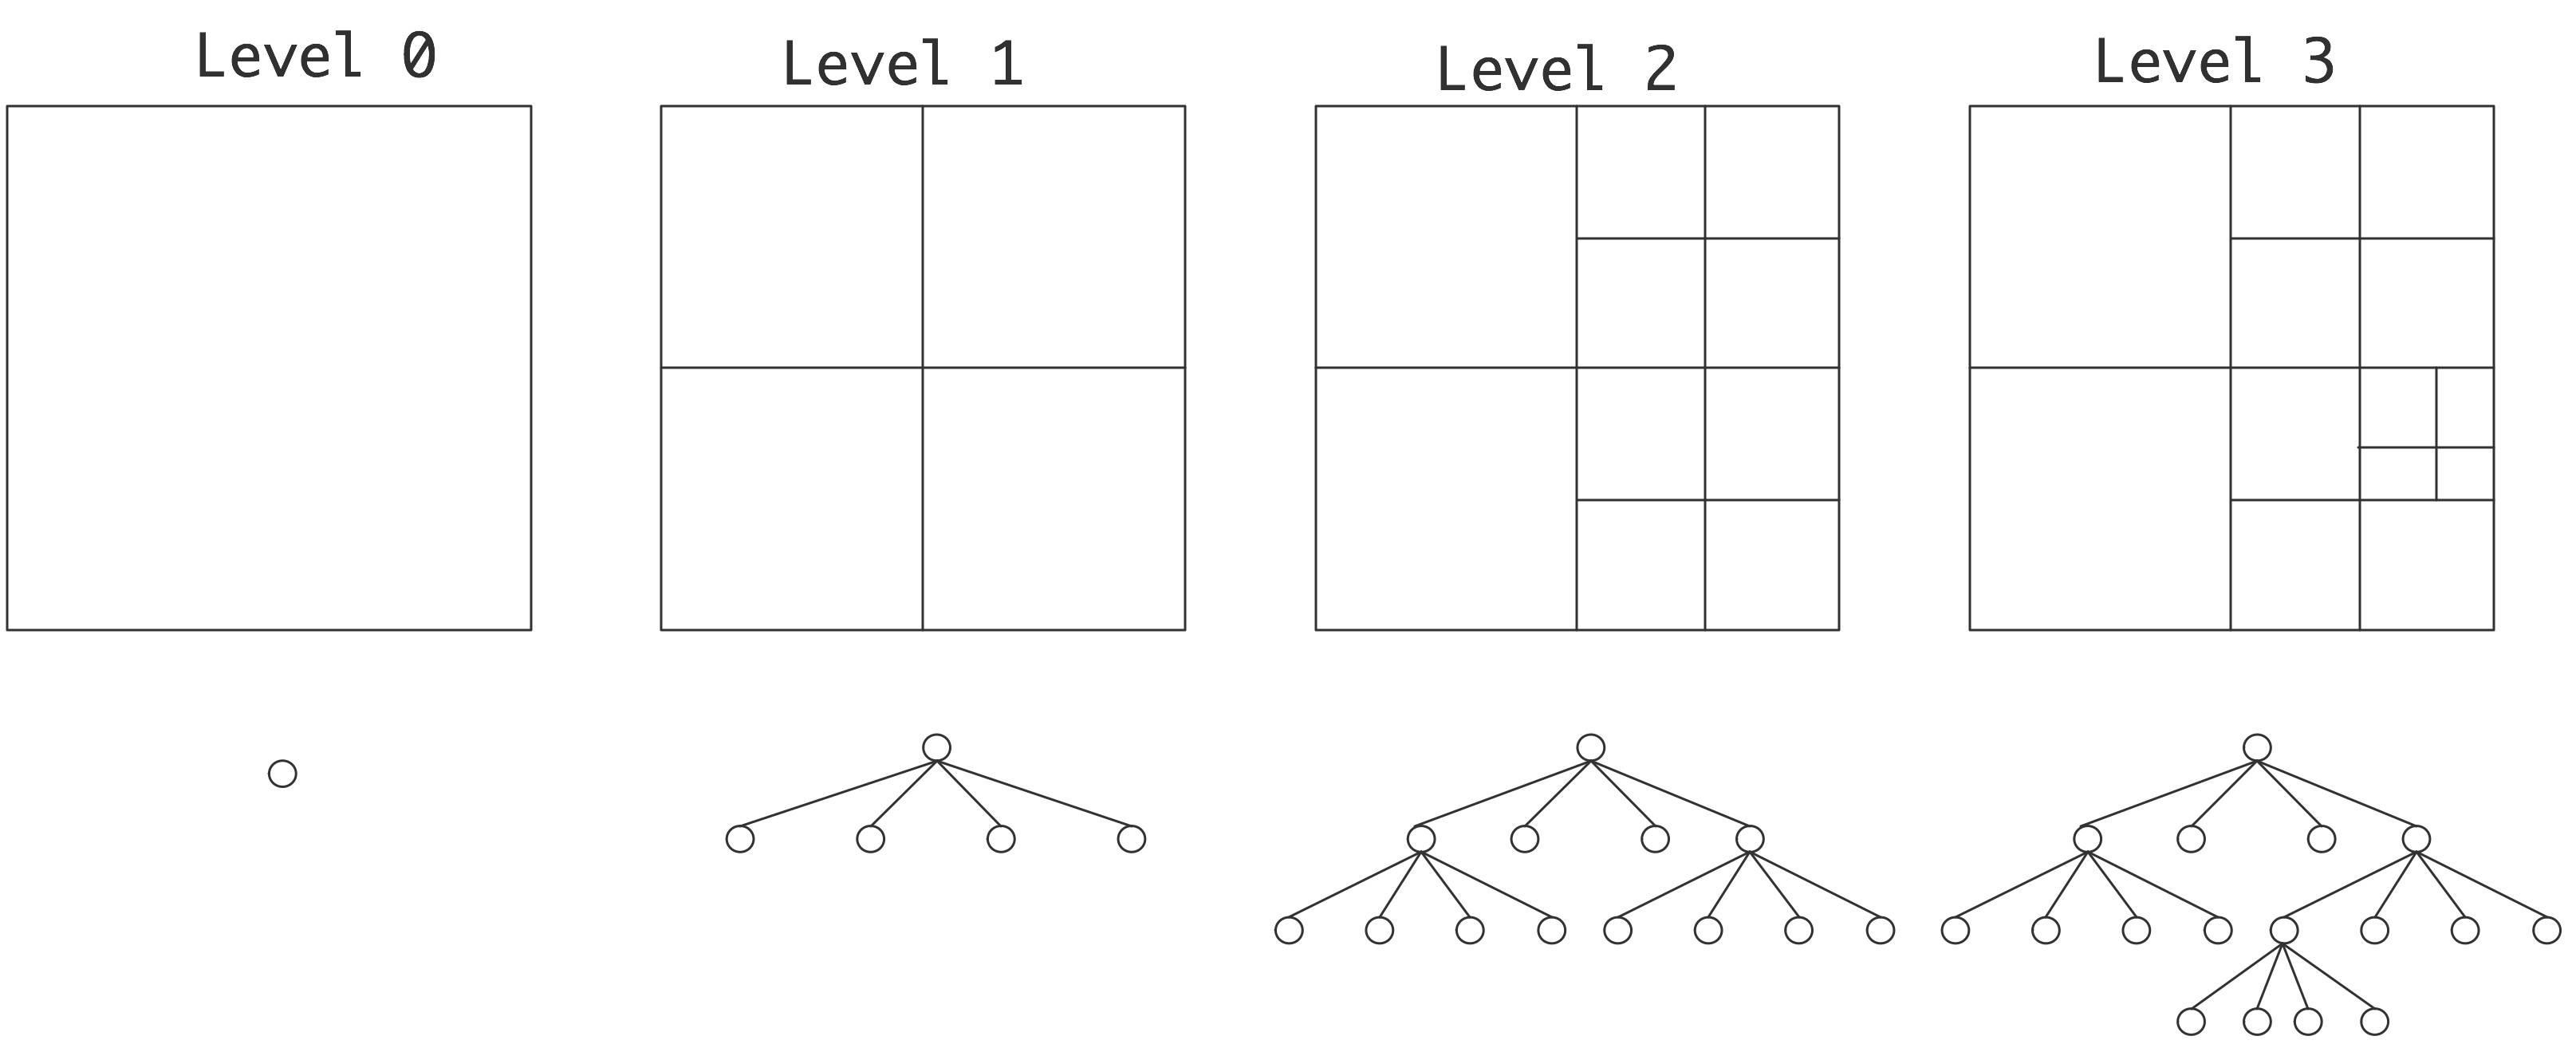
\includegraphics[scale=.09]{my_octree1}

  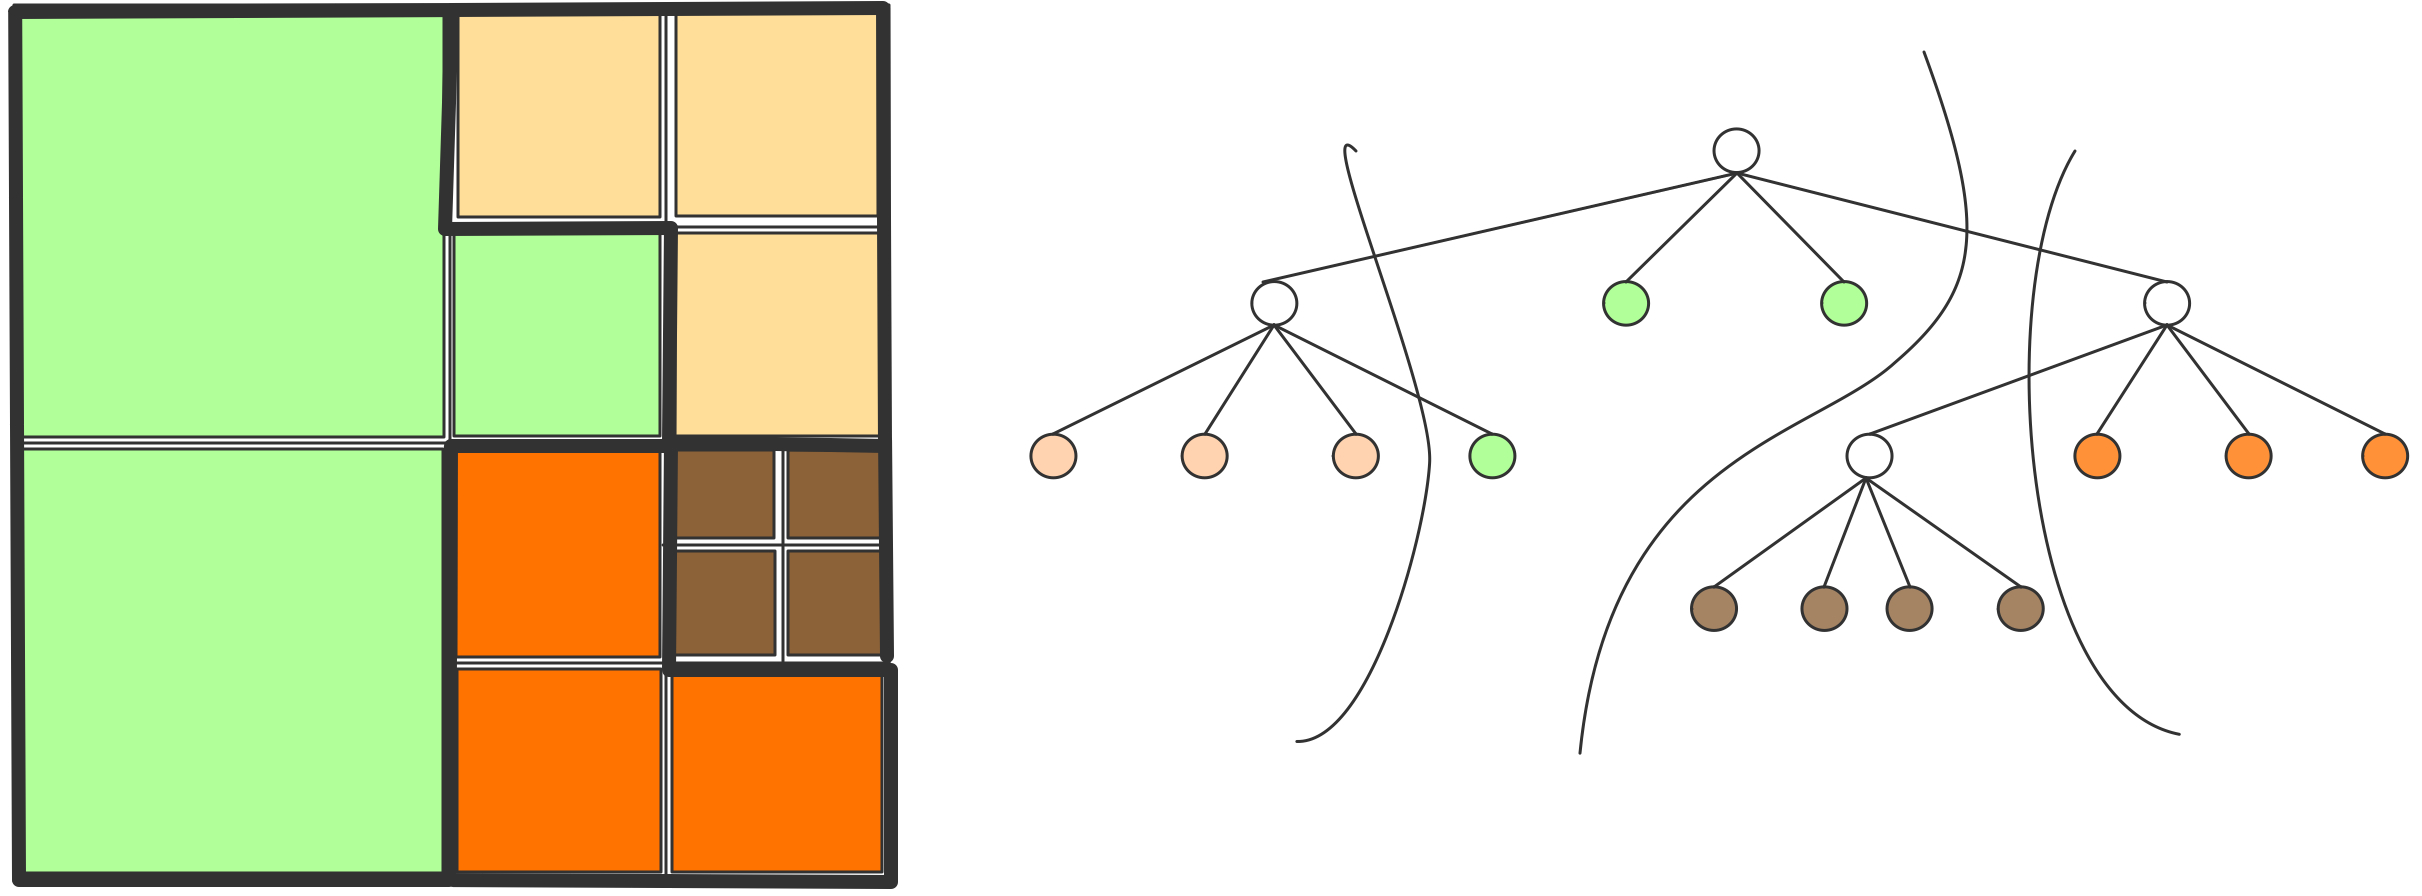
\includegraphics[scale=.1]{my_octree2}
\end{numberedframe}

\begin{numberedframe}{Assignment through Space-Filling Curve}
  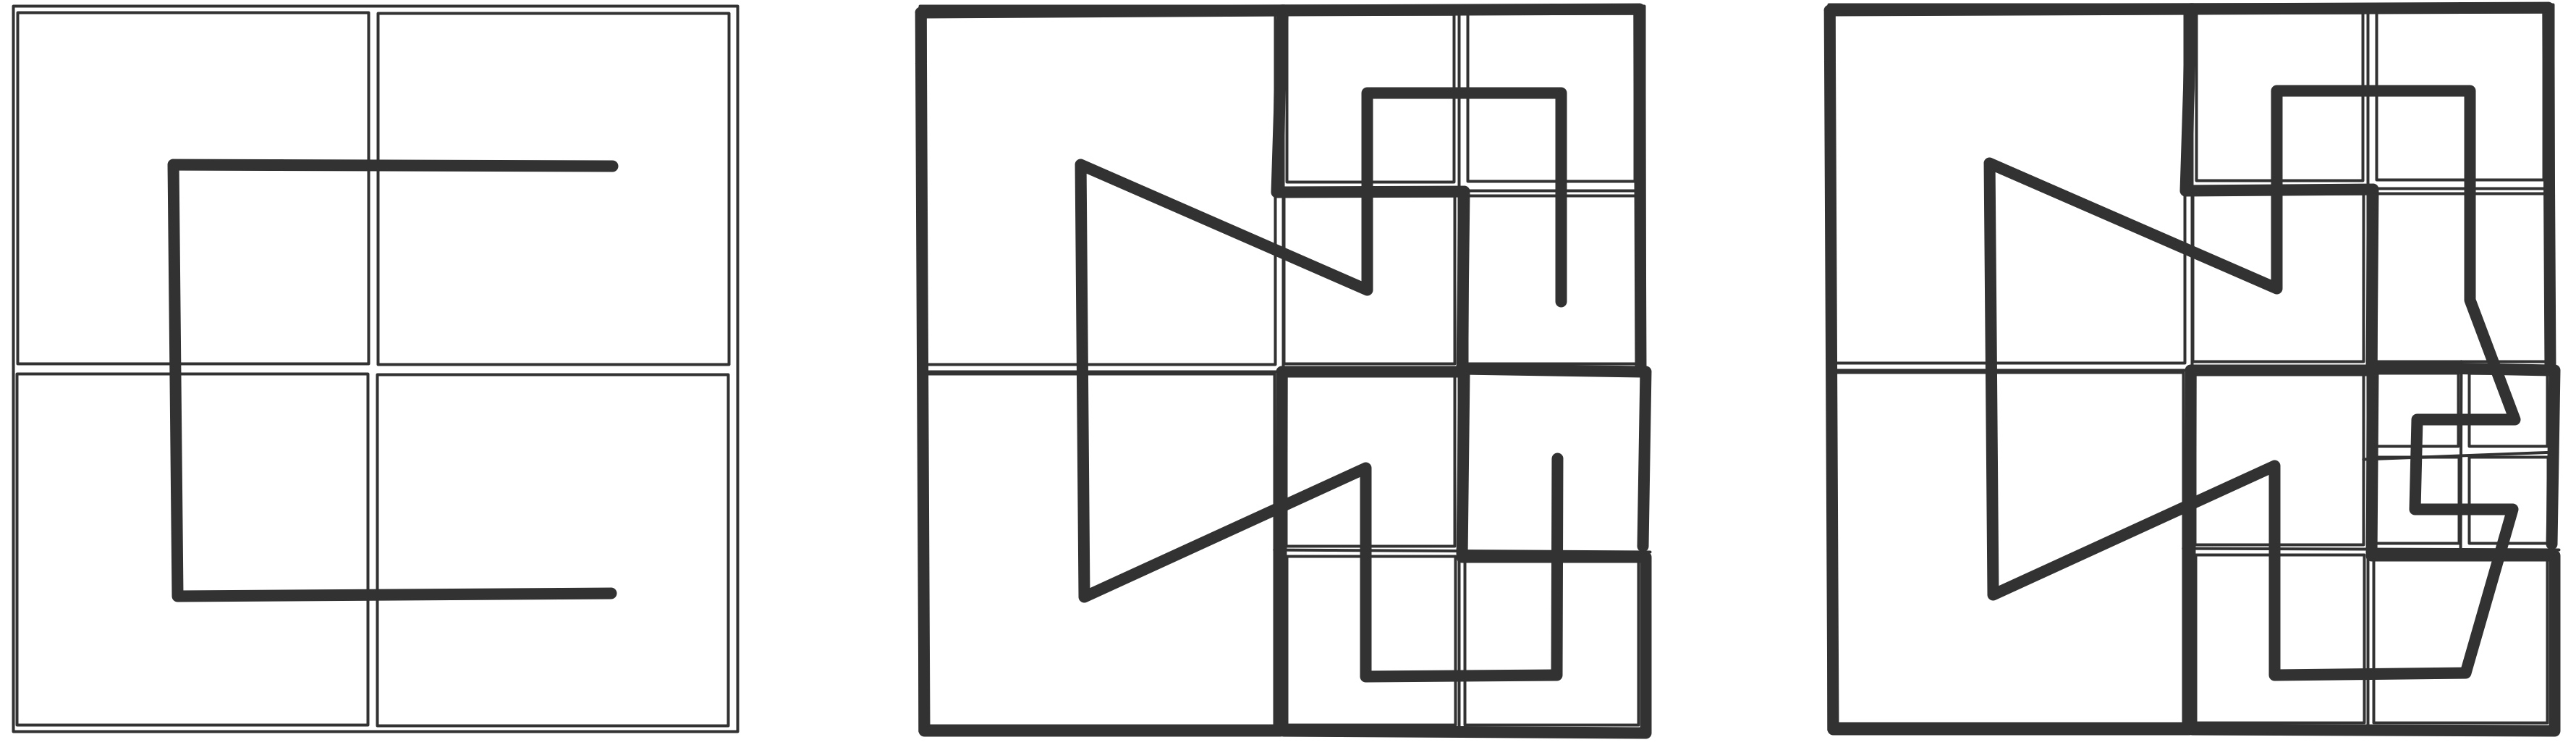
\includegraphics[scale=.08]{my_octree3_evolve}
  
  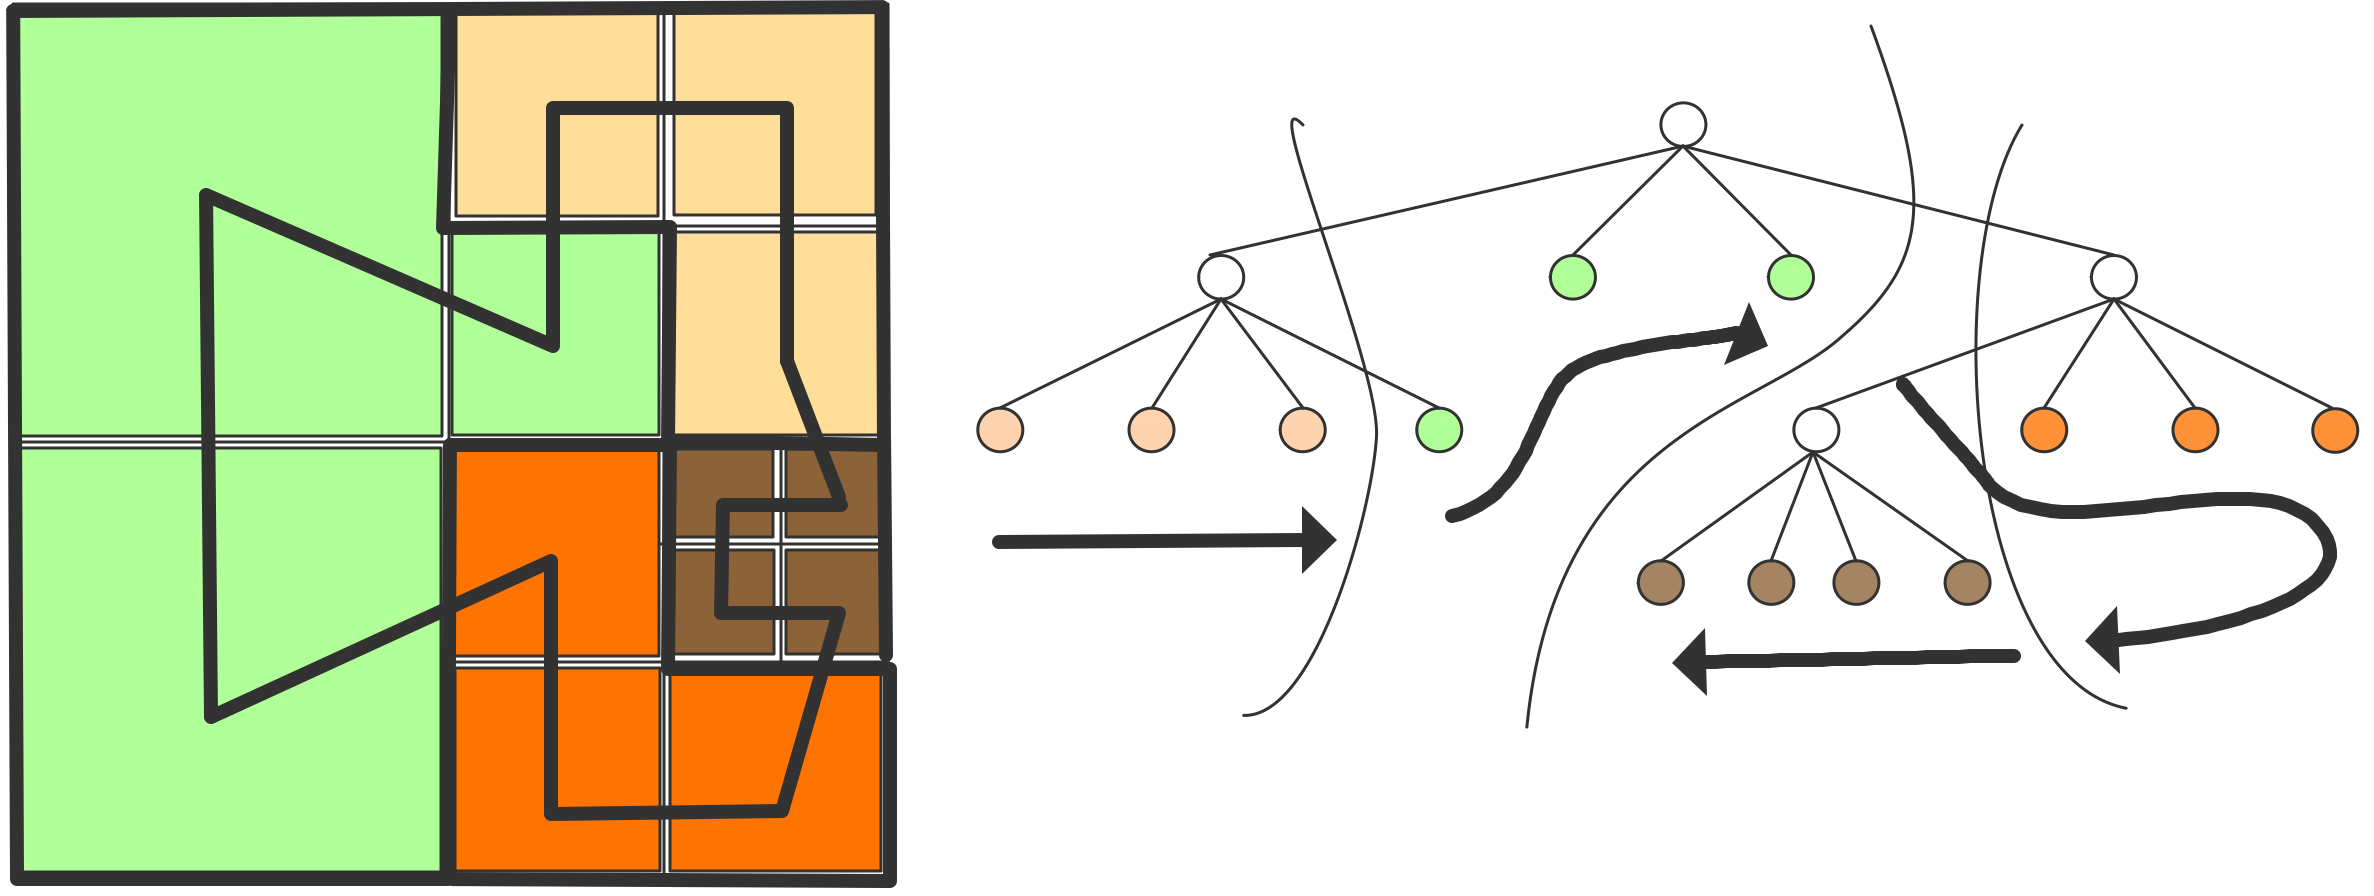
\includegraphics[scale=.08]{my_octree3}

\end{numberedframe}

\Level 2 {Domain partitioning by Fiedler vectors}

\begin{numberedframe}{Inspiration from physics}
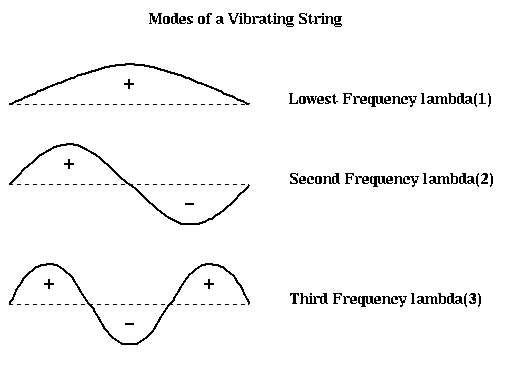
\includegraphics[scale=.5]{fiedlerstring}
\end{numberedframe}

\begin{numberedframe}{Graph laplacian}
\begin{itemize}
\item Set $G_{ij}=-1$ if edge $(i,j)$
\item Set $G_{ii}$ positive to give zero rowsums
\item First eigenvector is zero, positive eigenvector
\item Second eigenvector has pos/neg, divides in two
\item $n$-th eigenvector divides in $n$ parts
\end{itemize}
\end{numberedframe}

\begin{numberedframe}{Fiedler in a picture}
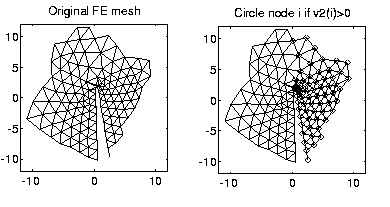
\includegraphics[scale=.7]{fiedlerdomain2}

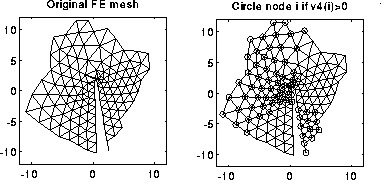
\includegraphics[scale=.7]{fiedlerdomain4}
\end{numberedframe}
